\documentclass{amsart}

\usepackage[margin=1.3in]{geometry}
\usepackage[english]{babel}
\usepackage{amsmath,amssymb}
\usepackage{graphicx}
\usepackage{xcolor}
\usepackage{comment}
\usepackage{booktabs}
\usepackage{tabularx}
\usepackage{enumitem}
\usepackage{tikz-cd}
\usepackage{bbm}
\usepackage{shuffle}
\usepackage{mathrsfs}
\usepackage{mathtools}
\usepackage{atbegshi}
\usepackage[autostyle]{csquotes}
\usepackage[toc,page]{appendix}
\usepackage{algorithm}
\usepackage[most]{tcolorbox}
\usepackage[
    colorlinks,
    citecolor=red,
    urlcolor=blue,
    bookmarks=false,
    hypertexnames=false
]{hyperref}
\usepackage{algpseudocode}
\usepackage[nameinlink,capitalize]{cleveref}

\newcommand{\ra}[1]{\renewcommand{\arraystretch}{#1}}

\newcommand{\assign}{:=}
\newcommand{\backassign}{=:}
\newcommand{\infixand}{\text{ and }}
\newcommand{\nobracket}{}

\newcommand{\tmmathbf}[1]{\ensuremath{\boldsymbol{#1}}}
\newcommand{\tmop}[1]{\ensuremath{\operatorname{#1}}}
\newcommand{\tmtextit}[1]{\text{\itshape #1}}
\newcommand{\vertiii}[1]{%
    {\left\vert\kern-0.25ex
     \left\vert\kern-0.25ex
     \left\vert #1
     \right\vert\kern-0.25ex
     \right\vert\kern-0.25ex
     \right\vert}%
}

\newtheorem{theorem}{Theorem}[section]
\newtheorem{lemma}[theorem]{Lemma}
\newtheorem{proposition}[theorem]{Proposition}
\newtheorem{corollary}[theorem]{Corollary}
\newtheorem{Assumption}[theorem]{Assumption}

\theoremstyle{definition}
\newtheorem{definition}[theorem]{Definition}
\newtheorem{notation}[theorem]{Notation}
\newtheorem{example}[theorem]{Example}

\theoremstyle{remark}
\newtheorem{remark}[theorem]{Remark}

\newtcolorbox{implrmk}{
    enhanced,
    breakable,
    colback=black!2,
    colframe=black!35,
    coltitle=black,
    boxrule=0.4pt,
    arc=1pt,
    left=6pt,
    right=6pt,
    top=5pt,
    bottom=5pt,
    before skip=8pt,
    after skip=8pt,
    fonttitle=\bfseries,
    title={Implementation}
}

\newcommand{\R}{\mathbb{R}}
\newcommand{\Z}{\mathbb{Z}}
\newcommand{\X}{\mathbb{X}}
\newcommand{\N}{\mathbb{N}}
\newcommand{\Y}{\mathbb{Y}}
\newcommand{\RPS}{\hat{\mathscr{C}}^{0,\alpha}_g}
\newcommand{\gRPS}{\mathscr{C}^{p\text{-var}}_g}
\newcommand{\dd}{\mathrm{d}}
\newcommand{\bmu}{\boldsymbol{\mu}}
\newcommand{\bgamma}{\boldsymbol{\gamma}}
\newcommand{\geoRP}[1]{\mathbf{#1}}
\newcommand{\YY}{\widehat{\mathbb{Y}}}
\newcommand{\ZZ}{\widehat{\mathbb{Z}}}
\newcommand{\Sig}[1]{\mathrm{Sig}(#1)}
\newcommand{\Sigsym}[1]{\widehat{\mathrm{Sig}}(#1)}
\newcommand{\RP}[1]{\mathbf{#1}}
\newcommand{\aRP}[1]{\widehat{\mathbf{#1}}}
\newcommand{\Gam}[1]{\Gamma(#1)}
\newcommand{\Gamsym}[1]{\widehat{\Gamma}(#1)}
\newcommand{\norm}[1]{\left\lVert #1 \right\rVert}

\newcommand{\gammashuffle}{{\,\bullet\,}}
\newcommand{\gammashufflesym}{{\,\widehat{\gammashuffle}\,}}
\newcommand{\symmetrizer}{{\,\widehat{\cdot}\,}}
\newcommand{\decomp}[1]{\Delta_{#1}}
\newcommand{\dott}{.}

\DeclareMathOperator*{\esssup}{ess\,sup}

\newcommand{\dsqcup}{%
    \sqcup
    \mathchoice
        {\mkern-7mu}
        {\mkern-7mu}
        {\mkern-3.2mu}
        {\mkern-3.8mu}
    \sqcup
}

\newcommand{\blue}[1]{{\color{blue}#1}}
\newcommand{\red}[1]{{\color{orange}#1}}
\newcommand{\orange}[1]{{\color{orange}#1}}
\newcommand{\wh}[1]{\widehat{#1}}

\begin{document}
\title[Signature Computations with Bidegree Truncation]
{A Technical Note on Signature Computations with Bidegree Truncation,
Coordinate Changes, and Symmetrization}
\author{Paul P. Hager \and Luca Pelizzari}
\date{\today}

\begin{abstract}
We give explicit data layouts and algorithms for signature computations with
bidegree truncation, the coordinate transformation introduced in
\cite{mainpaper}, and symmetrization over a partial alphabet.
The main conceptual difficulty is providing a contiguous array layout for
the bidegree-truncated tensors and expressing the basic tensor-algebra
operations, concatenation and shuffle, efficiently within this layout.
Our main approach is to introduce a rank axis that accounts for the
colexicographic ordering of the positions of the letters of the first
alphabet.
All operations can then be expressed as operations on the rank axis and as
permutations of the remaining dense tensor axes corresponding to the partial
alphabets.
We provide further implementation details for vectorized array execution
and discuss how word-parallel signature computation interfaces with the
ordered and partially symmetrized bidegree layouts.

\par\smallskip
\noindent\textbf{Disclaimer.}
To distinguish this paper from our other publications, we note that every
part of the manuscript was written and revised through iterative
human--machine cycles of prompting, generation, and review using the large
language models \emph{GBT-5.6 Sol} and \emph{Claude Fabel 5.0}. All algorithms proposed
in the paper were implemented in \texttt{tensordev}, and both the
implementations and the examples were verified through an extensive suite
of unit tests. The authors reviewed and approved all generated material and
take full responsibility for the final content.
\end{abstract}

\maketitle

\setcounter{secnumdepth}{3}
\setcounter{tocdepth}{2}
\tableofcontents

\section{Algebraic preliminaries}\label{sec:algebraic_preliminaries}

\subsection{Split alphabets, words, and bidegrees}\label{sec:split_alphabet}

Let
$\mathcal{A}
=
\mathcal{A}^{\prime}
\mathbin{\dot\cup}
\mathcal{A}^{\prime\prime}$
be a finite alphabet with both $\mathcal{A}^{\prime}$ and
$\mathcal{A}^{\prime\prime}$ nonempty, and define
$d := |\mathcal{A}|$. We write
$\blue{i}\in\mathcal{A}^{\prime}$ and
$\orange{j}\in\mathcal{A}^{\prime\prime}$, and denote by
$\mathcal{W}_{\mathcal{A}}$ the set of finite words over $\mathcal{A}$,
including the empty word $\varnothing$. For
$w,v \in \mathcal{W}_{\mathcal{A}}$, we write
$wv \in \mathcal{W}_{\mathcal{A}}$ for their concatenation.

For $w\in\mathcal{W}_{\mathcal{A}}$, let
$|w|_{\mathcal{A}^{\prime}}$ and
$|w|_{\mathcal{A}^{\prime\prime}}$ be the numbers of letters of $w$ in
$\mathcal{A}^{\prime}$ and $\mathcal{A}^{\prime\prime}$, respectively. We
call
$\bigl(
|w|_{\mathcal{A}^{\prime}},
|w|_{\mathcal{A}^{\prime\prime}}
\bigr) \in \mathbb{N}_0\times\mathbb{N}_0$
the \emph{bidegree} of $w$. In particular,
$|w|
=
|w|_{\mathcal{A}^{\prime}}
+
|w|_{\mathcal{A}^{\prime\prime}}$.
Every word $w$ of bidegree $(n,m)$ has a unique decomposition
\[
    w
    =
    w_0\blue{i_1}w_1\cdots\blue{i_n}w_n,
    \qquad
    w_0,\ldots,w_n
    \in
    \mathcal{W}_{\mathcal{A}^{\prime\prime}},
    \quad
    \blue{i_1},\ldots,\blue{i_n}
    \in
    \mathcal{A}^{\prime},
\]
with $|w_0|+\cdots+|w_n| = m$.
We write
\[
    \decomp{\mathcal{A}^{\prime}}(w)
    :=
    \left(
        (w_0,\ldots,w_n),
        \blue{i_1}\cdots\blue{i_n}
    \right).
\]
For $n=0$, this means
$\decomp{\mathcal{A}^{\prime}}(w)=((w),\varnothing)$.

A path $Y\colon[s,t]\to\mathbb{R}^{d}$ whose coordinates are indexed by
$\mathcal{A}$ is written as $Y=(A,X)$, where $A$ consists of the coordinates
indexed by $\mathcal{A}^{\prime}$ and $X$ of those indexed by
$\mathcal{A}^{\prime\prime}$.

\subsection{Tensor algebra, signatures and shuffle}
\label{sec:tensor_signatures}

Let $(e_i)_{i\in\mathcal{A}}$ be the canonical basis of
$\mathbb{R}^{d}$. For
$w=i_1\cdots i_r\in\mathcal{W}_{\mathcal{A}}$, write
$e_w:=e_{i_1}\otimes\cdots\otimes e_{i_r}$ and
$e_{\emptyset}:=1$. The extended tensor algebra is
\[
    T((\mathbb{R}^{d}))
    :=
    \prod_{r\geq0}
    (\mathbb{R}^{d})^{\otimes r},
    \qquad
    (\mathbb{R}^{d})^{\otimes0}
    :=
    \mathbb{R},
\]
with concatenation product $\otimes$, determined by
$e_u\otimes e_v=e_{uv}$.

The free associative algebra
$\mathbb{R}\langle\mathcal{A}\rangle$ is the linear span of
$\mathcal{W}_{\mathcal{A}}$.
We identify a word with the corresponding coordinate functional on
$T((\mathbb{R}^{d}))$ and write $\langle w,\mathbf{a}\rangle$ for the
coefficient of $e_w$ in $\mathbf{a}$. This extends to the bilinear pairing
\[
    \langle \,\cdot\,,\,\cdot\,\rangle
    \colon
    \mathbb{R}\langle\mathcal{A}\rangle
    \times
    T((\mathbb{R}^{d}))
    \longrightarrow
    \mathbb{R}.
\]

Let $Y\in C^{1\text{-var}}([s,t],\mathbb{R}^{d})$. For
$w=i_1\cdots i_n$, its signature coordinate is
\[
    \left\langle
        w,
        \Sig{Y}_{s,t}
    \right\rangle
    :=
    \int_{s<u_1<\cdots<u_n<t}
    \dd Y^{i_1}_{u_1}\cdots\dd Y^{i_n}_{u_n},
    \qquad
    \left\langle
        \varnothing,
        \Sig{Y}_{s,t}
    \right\rangle
    :=
    1.
\]
The signature is the tensor series
$\Sig{Y}_{s,t}
=
\sum_{w\in\mathcal{W}_{\mathcal{A}}}
\langle w,\Sig{Y}_{s,t}\rangle e_w$.
For $s\leq u\leq t$, Chen's identity states that
\[
    \Sig{Y}_{s,t}
    =
    \Sig{Y}_{s,u}
    \otimes
    \Sig{Y}_{u,t}.
\]
If $Y_{s,\cdot}$ is linear on $[s,t]$, then
\[
    \Sig{Y}_{s,t}
    =
    \exp_{\otimes}(Y_{s,t})
    :=
    \sum_{r=0}^{\infty}
    \frac{Y_{s,t}^{\otimes r}}{r!}.
\]
Consequently, the signature of a piecewise linear path is obtained by tensor exponentiation of each increment and combining the
segment signatures by concatenation.

The shuffle product on
$\mathbb{R}\langle\mathcal{A}\rangle$ is determined recursively by
\[
    w\shuffle\emptyset
    =
    \emptyset\shuffle w
    =
    w,
    \qquad
    wi\shuffle vj
    =
    (w\shuffle vj)i
    +
    (wi\shuffle v)j,
\]
for $w,v\in\mathcal{W}_{\mathcal{A}}$ and $i,j\in\mathcal{A}$. Signature
coordinates satisfy the shuffle identity
\[
    \left\langle
        u,
        \Sig{Y}_{s,t}
    \right\rangle
    \left\langle
        v,
        \Sig{Y}_{s,t}
    \right\rangle
    =
    \left\langle
        u\shuffle v,
        \Sig{Y}_{s,t}
    \right\rangle.
\]

\subsection{Bidegree truncation}\label{sec:bigraded_truncation}

For the alphabet split
$\mathcal{A}
=
\mathcal{A}^{\prime}
\mathbin{\dot\cup}
\mathcal{A}^{\prime\prime}$
and $n,m\in\mathbb{N}_0$, define the homogeneous bidegree spaces
\begin{align*}
     T^{(n,m)}(\mathbb{R}^{d})
    :=&
    \operatorname{span}
    \left\{
        e_w:
        |w|_{\mathcal{A}^{\prime}}=n,
        \quad
        |w|_{\mathcal{A}^{\prime\prime}}=m
    \right\},
    \\
    \mathbb{R}^{(n,m)}\langle\mathcal{A}\rangle
    :=&
    \operatorname{span}
    \left\{
        w:
        |w|_{\mathcal{A}^{\prime}}=n,
        \quad
        |w|_{\mathcal{A}^{\prime\prime}}=m
    \right\}.
\end{align*}
For $\mathbf{a}\in T((\mathbb{R}^{d}))$, we write
$\mathbf{a}^{(n,m)}\in T^{(n,m)}(\mathbb{R}^{d})$ for its homogeneous
component of bidegree $(n,m)$, and analogously for elements of
$\mathbb{R}\langle\mathcal{A}\rangle$.
For truncation levels $N,M\in\mathbb{N}_0$, define the bigraded truncated
tensor algebra and dual word space by
\[
    T^{N,M}(\mathbb{R}^{d})
    :=
    \bigoplus_{n=0}^{N}
    \bigoplus_{m=0}^{M}
    T^{(n,m)}(\mathbb{R}^{d}),
    \qquad
    \mathbb{R}^{N,M}\langle\mathcal{A}\rangle
    :=
    \bigoplus_{n=0}^{N}
    \bigoplus_{m=0}^{M}
    \mathbb{R}^{(n,m)}\langle\mathcal{A}\rangle.
\]
We denote the corresponding projections by $\pi^{N,M}$, so that
\[
    \pi^{N,M}\mathbf{a}
    =
    \sum_{n=0}^{N}
    \sum_{m=0}^{M}
    \mathbf{a}^{(n,m)},
\]
and use the same notation for the projection on
$\mathbb{R}\langle\mathcal{A}\rangle$.
Since concatenation and shuffle add bidegrees, they descend to the bigraded
truncation through
\[
    \mathbf{a}\otimes_{N,M}\mathbf{b}
    :=
    \pi^{N,M}
    \bigl(
        \mathbf{a}\otimes\mathbf{b}
    \bigr),
    \qquad
    \alpha\shuffle_{N,M}\beta
    :=
    \pi^{N,M}
    \bigl(
        \alpha\shuffle\beta
    \bigr).
\]
Both truncated products are associative and have the empty word as their
unit.

We write
$\Sig{Y}^{N,M}_{s,t}
:=
\pi^{N,M}\Sig{Y}_{s,t}$. Since the discarded bidegrees form an ideal for
concatenation, Chen's identity descends to
\[
    \Sig{Y}^{N,M}_{s,t}
    =
    \Sig{Y}^{N,M}_{s,u}
    \otimes_{N,M}
    \Sig{Y}^{N,M}_{u,t}.
\]
Moreover, for words $u,v$ satisfying
$|u|_{\mathcal{A}^{\prime}}+|v|_{\mathcal{A}^{\prime}}\leq N$ and
$|u|_{\mathcal{A}^{\prime\prime}}+|v|_{\mathcal{A}^{\prime\prime}}\leq M$,
the shuffle identity becomes
\[
    \big\langle u,\Sig{Y}^{N,M}_{s,t}\big\rangle
    \big\langle v,\Sig{Y}^{N,M}_{s,t}\big\rangle
    =
    \big\langle
        u\shuffle v,
        \Sig{Y}^{N,M}_{s,t}
    \big\rangle.
\]
For $K\in\mathbb{N}_0$, the total-degree truncated tensor algebra of degree
$K$ is
\[
    T^K(\mathbb{R}^{d})
    :=
    \bigoplus_{r=0}^K(\mathbb{R}^{d})^{\otimes r},
    \qquad
    \pi_K
    \colon
    T((\mathbb{R}^{d}))
    \to
    T^K(\mathbb{R}^{d}),
    \qquad
    \mathbf{a}\otimes_K\mathbf{b}
    :=
    \pi_K(\mathbf{a}\otimes\mathbf{b}).
\]
For $K=N+M$, it is the smallest total-degree truncated tensor algebra
containing $T^{N,M}(\mathbb{R}^{d})$.

\subsection{Shear coordinate transformation}
\label{sec:shear_coordinate_transformation}

We recall the coordinate transformation associated with the alphabet split
$(\mathcal{A}^{\prime},\mathcal{A}^{\prime\prime})$ introduced in
\cite{mainpaper}, which we call the \emph{shear coordinate transformation}
for simplicity; cf.~\cite[Remark~3.3]{mainpaper}. Specifically, the
transformation is given by a graded linear automorphism
$\Psi:T((\mathbb{R}^d))\to T((\mathbb{R}^d))$ and the induced pairing on
$\mathbb{R}\langle\mathcal{A}\rangle\times T((\mathbb{R}^d))$ defined by
\[
    \langle \alpha,\mathbf{a}\rangle_{\Psi}
    :=
    \langle \alpha,\Psi(\mathbf{a})\rangle,
    \qquad
    \alpha\in\mathbb{R}\langle\mathcal{A}\rangle,
    \quad
    \mathbf{a}\in T((\mathbb{R}^d)).
\]
The transformation is characterized by the signature coefficients in the
resulting coordinates
$\langle\cdot,\cdot\rangle_{\Psi}$. More precisely, let
$Y=(A,X)\in C^{1\text{-var}}([s,t],\mathbb{R}^{d})$. For
$w\in\mathcal{W}_{\mathcal{A}}$, write
$\decomp{\mathcal{A}^{\prime}}(w)
    =
    \left(
        (w_0,\ldots,w_n),
        \blue{i_1}\cdots\blue{i_n}
    \right)$.
Set $\Delta^n_{s,t}:=\{(t_1,\ldots,t_n):s<t_1<\cdots<t_n<t\}$, with the
usual empty-simplex convention for $n=0$.
Then the corresponding signature coordinate is
\[
    \big\langle w,\Sig{Y}_{s,t}\big\rangle_{\Psi}
    =
    \big\langle w_n,\Sig{X}_{s,t}\big\rangle
    \int_{\Delta^n_{s,t}}
    \prod_{j=1}^{n}
    \big\langle w_{j-1},\Sig{X}_{s,t_j}\big\rangle
    \,\dd A_{t_j}^{\blue{i_j}}.
\]
Since $\Psi$ is an invertible graded linear map, its inverse
$\Psi^{-1}:T((\mathbb{R}^d))\to T((\mathbb{R}^d))$ is graded as well. We
recall the recursive algebraic definitions of both maps in
\cref{sec:shear_coordinate_computation}. Moreover, both maps preserve
bidegrees, that is, for every
$\mathbf{a}\in T((\mathbb{R}^d))$ and $(n,m)\in\mathbb{N}_0^2$,
\[
    \bigl(\Psi(\mathbf{a})\bigr)^{(n,m)}
    =
    \Psi\bigl(\mathbf{a}^{(n,m)}\bigr),
    \qquad
    \bigl(\Psi^{-1}(\mathbf{a})\bigr)^{(n,m)}
    =
    \Psi^{-1}\bigl(\mathbf{a}^{(n,m)}\bigr).
\]
Consequently, they restrict to inverse linear automorphisms of
$T^{N,M}(\mathbb{R}^d)$.

\subsection{Partial symmetrization and quotient normal forms}
\label{sec:partial_symmetrization}

Following \cite{mainpaper}, we partially symmetrize by imposing
commutativity between adjacent letters in
$\mathcal{A}^{\prime\prime}$. Let
\[
    \mathcal{J}_{\mathcal{A}^{\prime\prime}}
    :=
    \operatorname{span}
    \left\{
        u\bigl(
            \orange{i}\orange{j}
            -
            \orange{j}\orange{i}
        \bigr)v
        :
        u,v\in\mathcal{W}_{\mathcal{A}},
        \quad
        \orange{i},\orange{j}\in\mathcal{A}^{\prime\prime}
    \right\},
    \qquad
    \mathbb{R}_{\mathcal{A}^{\prime\prime}}
    \langle\mathcal{A}\rangle
    :=
    \mathbb{R}\langle\mathcal{A}\rangle
    /
    \mathcal{J}_{\mathcal{A}^{\prime\prime}},
\]
and denote the quotient class of a word $w$ by $[w]$. If $\decomp{\mathcal{A}^{\prime}}(w)
    =
    \bigl(
        (w_0,\ldots,w_n),
        \blue{i_1}\cdots\blue{i_n}
    \bigr),$
then
\[
    [w]
    =
    [w_0]\blue{i_1}[w_1]\cdots
    \blue{i_n}[w_n].
\]
Thus only permutations within an
$\mathcal{A}^{\prime\prime}$-block are identified, while the order of the
blocks and of the $\mathcal{A}^{\prime}$-letters is retained.
The ideal $\mathcal{J}_{\mathcal{A}^{\prime\prime}}$ is bigraded, and the
quotient therefore inherits the bidegree decomposition. For
$n,m\in\mathbb{N}_0$, define
\[
    \mathbb{R}_{\mathcal{A}^{\prime\prime}}^{(n,m)}
    \langle\mathcal{A}\rangle
    :=
    \operatorname{span}
    \left\{
        [w]:
        |w|_{\mathcal{A}^{\prime}}=n,
        \quad
        |w|_{\mathcal{A}^{\prime\prime}}=m
    \right\}.
\]
On the tensor side, define
\[
    \widehat{T}^{(n,m)}(\mathbb{R}^{d})
    :=
    \operatorname{span}
    \left\{
        e_{[w]}:
        |w|_{\mathcal{A}^{\prime}}=n,
        \quad
        |w|_{\mathcal{A}^{\prime\prime}}=m
    \right\},
\]
and
\[
    T_{\mathcal{A}^{\prime\prime}}((\mathbb{R}^{d}))
    :=
    \prod_{n,m\geq0}
    \widehat{T}^{(n,m)}(\mathbb{R}^{d}).
\]
Partial symmetrization is the bidegree-preserving linear map
\[
    \symmetrizer:
    T((\mathbb{R}^{d}))
    \longrightarrow
    T_{\mathcal{A}^{\prime\prime}}((\mathbb{R}^{d})),
    \qquad
    e_w\longmapsto e_{[w]}.
\]
For $\mathbf{a}\in T((\mathbb{R}^{d}))$, we write
$\widehat{\mathbf{a}}:=\symmetrizer(\mathbf{a})$. The induced pairing is
given by
\[
    \big\langle
        [w],
        \widehat{\mathbf{a}}
    \big\rangle
    =
    \sum_{[v]=[w]}
    \big\langle
        v,
        \mathbf{a}
    \big\rangle.
\]
The graded transpose of $\symmetrizer$ is the injective map
$\symmetrizer^{\ast}:\mathbb{R}_{\mathcal{A}^{\prime\prime}}
\langle\mathcal{A}\rangle\to\mathbb{R}\langle\mathcal{A}\rangle$,
characterized by
$\symmetrizer^{\ast}([w])=\sum_{[v]=[w]}v$. Consequently,
$\langle\alpha,\widehat{\mathbf{a}}\rangle
=\langle\symmetrizer^{\ast}(\alpha),\mathbf{a}\rangle$.
Each distinct ordered representative occurs exactly once in this sum, so no
factorial weight is introduced. The map $\symmetrizer^{\ast}$ is an adjoint
lift, not an inverse of $\symmetrizer$.
For $N,M\in\mathbb{N}_0$, define the bigraded truncated partially
symmetrized tensor algebra and its dual word space by
\[
    \widehat{T}^{N,M}(\mathbb{R}^{d})
    :=
    \bigoplus_{n=0}^{N}
    \bigoplus_{m=0}^{M}
    \widehat{T}^{(n,m)}(\mathbb{R}^{d}),
    \qquad
    \mathbb{R}_{\mathcal{A}^{\prime\prime}}^{N,M}
    \langle\mathcal{A}\rangle
    :=
    \bigoplus_{n=0}^{N}
    \bigoplus_{m=0}^{M}
    \mathbb{R}_{\mathcal{A}^{\prime\prime}}^{(n,m)}
    \langle\mathcal{A}\rangle.
\]
Equivalently,
\(
    \widehat{T}^{N,M}(\mathbb{R}^{d})
    =
    \symmetrizer
    \bigl(
        T^{N,M}(\mathbb{R}^{d})
    \bigr).
\)
For
$\alpha
=
(\alpha_{\orange{i}})_{\orange{i}\in\mathcal{A}^{\prime\prime}}
\in
\mathbb{N}_0^{\mathcal{A}^{\prime\prime}}$,
we identify $\alpha$ with the common quotient class of all
$\mathcal{A}^{\prime\prime}$-words containing each letter
$\orange{i}$ exactly $\alpha_{\orange{i}}$ times, and write
\[
    |\alpha|
    :=
    \sum_{\orange{i}\in\mathcal{A}^{\prime\prime}}
    \alpha_{\orange{i}}.
\]
Every quotient word of bidegree $(n,m)$ has a unique \emph{normal form}
\[
    \alpha_0\blue{i_1}\alpha_1\cdots
    \blue{i_n}\alpha_n,
\]
where
$\alpha_0,\ldots,\alpha_n
\in\mathbb{N}_0^{\mathcal{A}^{\prime\prime}}$,
$\blue{i_1},\ldots,\blue{i_n}\in\mathcal{A}^{\prime}$, and $|\alpha_0| + \cdots + |\alpha_n|=m$.

\subsection{Coordinate changes, quotients, and induced products}
\label{sec:coordinate_changes_and_products}

In standard coordinates the signature is $\Sig{Y}$, while in shear
coordinates it is $\Psi(\Sig{Y})$, since
\[
    \big\langle
        w,
        \Sig{Y}_{s,t}
    \big\rangle_{\Psi}
    =
    \big\langle
        w,
        \Psi\bigl(\Sig{Y}_{s,t}\bigr)
    \big\rangle.
\]
The partially symmetrized signature is the quotient tensor series
\[
    \Sigsym{Y}_{s,t}
    :=
    \widehat{\Sig{Y}_{s,t}}.
\]
As shown in \cite{mainpaper}, the tensor-side kernel
$\mathcal{I}_{\mathcal{A}^{\prime\prime}}
:=
\ker(\symmetrizer)$
is invariant under $\Psi$ and $\Psi^{-1}$. Hence, they descend to inverse
linear automorphisms $\widehat{\Psi}$ and $\widehat{\Psi}^{-1}$ satisfying
\[
    \widehat{\Psi}(\widehat{\mathbf{a}})
    =
    \widehat{\Psi(\mathbf{a})},
    \qquad
    \widehat{\Psi}^{-1}(\widehat{\mathbf{a}})
    =
    \widehat{\Psi^{-1}(\mathbf{a})}.
\]
The corresponding shear pairing on the quotient is therefore defined by
\[
    \big\langle
        \alpha,
        \widehat{\mathbf{a}}
    \big\rangle_{\Psi}
    :=
    \big\langle
        \alpha,
        \widehat{\Psi}(\widehat{\mathbf{a}})
    \big\rangle,
    \qquad
    \alpha
    \in
    \mathbb{R}_{\mathcal{A}^{\prime\prime}}
    \langle\mathcal{A}\rangle.
\]
The standard and shear coordinates, before and after partial symmetrization,
each carry a tensor product governing the corresponding Chen
identity and a dual product governing multiplication of coordinate
functionals. The products used below are summarized as follows:
\[
\begin{array}{c|c|c}
    \text{coordinates}
    &
    \text{group law}
    &
    \text{dual product}
    \\
    \hline
    \Sig{Y}
    &
    \otimes
    &
    \shuffle
    \\
    \Psi(\Sig{Y})
    &
    \odot
    &
    \gammashuffle
    \\
    \Sigsym{Y}
    &
    \widehat{\otimes}
    &
    \widehat{\shuffle}
    \\
    \widehat{\Psi}(\Sigsym{Y})
    &
    \widehat{\odot}
    &
    \gammashufflesym
\end{array}
\]
The tensor products are related by coordinate transport and passage to the
quotient:
\[
    \mathbf{a}\odot\mathbf{b}
    :=
    \Psi
    \bigl(
        \Psi^{-1}(\mathbf{a})
        \otimes
        \Psi^{-1}(\mathbf{b})
    \bigr),
    \qquad
    \widehat{\mathbf{a}}
    \,\widehat{\otimes}\,
    \widehat{\mathbf{b}}
    :=
    \widehat{\mathbf{a}\otimes\mathbf{b}},
    \qquad
    \widehat{\mathbf{a}}
    \,\widehat{\odot}\,
    \widehat{\mathbf{b}}
    :=
    \widehat{\Psi}
    \bigl(
        \widehat{\Psi}^{-1}(\widehat{\mathbf{a}})
        \,\widehat{\otimes}\,
        \widehat{\Psi}^{-1}(\widehat{\mathbf{b}})
    \bigr).
\]
The products
$\shuffle$, $\gammashuffle$, $\widehat{\shuffle}$, and
$\gammashufflesym$ are the corresponding graded dual products. Thus, for
each row of the table, denoting its entries by
$\mathbf{S}$, $\circledast$, and $\star$, respectively, we have
\[
    \mathbf{S}_{s,t}
    =
    \mathbf{S}_{s,u}
    \circledast
    \mathbf{S}_{u,t},
    \qquad
    \big\langle\alpha,\mathbf{S}_{s,t}\big\rangle
    \big\langle\beta,\mathbf{S}_{s,t}\big\rangle
    =
    \big\langle
        \alpha\star\beta,
        \mathbf{S}_{s,t}
    \big\rangle,
\]
for $Y\in C^{1\text{-var}}([s,t],\mathbb{R}^d)$, $s\leq u\leq t$, and
$\alpha,\beta$ in the corresponding dual word space. In the second and
fourth rows, the standard pairing with the displayed transformed tensor is,
equivalently, the $\Psi$-pairing with the corresponding untransformed
signature tensor.

The coordinate changes and partial symmetrization preserve bidegrees, while
all tensor and dual products add bidegrees. They therefore descend to the
corresponding bigraded truncations. We denote the resulting products by
\[
    \otimes_{N,M},
    \qquad
    \odot_{N,M},
    \qquad
    \widehat{\otimes}_{N,M},
    \qquad
    \widehat{\odot}_{N,M},
    \qquad
    \shuffle_{N,M},
    \qquad
    \gammashuffle_{N,M},
    \qquad
    \widehat{\shuffle}_{N,M},
    \qquad
    \gammashufflesym_{N,M}.
\]
In the following sections, we revisit these products in their respective
coordinate layouts and derive explicit algorithms for their computation.

\section{Data layouts}
\label{sec:data_layouts}

For a total-degree truncated tensor, each homogeneous component
$(\mathbb{R}^{d})^{\otimes r}$ has the canonical dense array layout with
shape
\[
    \underbrace{d\times\cdots\times d}_{r\text{ times}}.
\]
For a fixed bidegree $(n,m)$, however, the
$\mathcal{A}^{\prime}$- and $\mathcal{A}^{\prime\prime}$-letters may occur
in different relative positions.
One placement pattern, in bidegree $(2,3)$ for example
\[
    \orange{\bullet}\,
    \blue{\bullet}\,
    \orange{\bullet}\,
    \orange{\bullet}\,
    \blue{\bullet},
\]
specifies which two positions are occupied by
$\mathcal{A}^{\prime}$-letters and which three by
$\mathcal{A}^{\prime\prime}$-letters. Once the placement is fixed, the
corresponding coordinates of the bidegree tensor have the usual dense tensor
layout
\[
    (\mathbb{R}^{|\mathcal{A}^{\prime}|})^{\otimes n}
    \otimes
    (\mathbb{R}^{|\mathcal{A}^{\prime\prime}|})^{\otimes m}.
\]
We therefore store a tensor of bidegree $(n,m)$ as a collection of such
dense subtensors, together with an additional axis indexing the possible
placements. Under partial symmetrization, the ordered
$\mathcal{A}^{\prime\prime}$-indices within each block are replaced by
their multiplicity multi-indices, and the placement axis is replaced by an
axis indexing the resulting multiset placements. The following subsections
make these two indexing sets explicit and assign them compact integer ranks.

\subsection{Colexicographic ranking}
\label{sec:colexicographic_ranking}

For integers $N\geq0$ and $0\leq r\leq N$, let
\[
    P=\{p_1<\cdots<p_r\}
    \subseteq
    \{1,\ldots,N\}
\]
be an $r$-element subset. Its colexicographic rank is defined by
\cite[Theorem~L and Eq.~(20), p.~360]{knuth2011taocp4a}
\[
    \operatorname{rk}(P)
    :=
    \sum_{s=1}^{r}
    \binom{p_s-1}{s}.
\]
This defines a bijection from the $r$-element subsets of
$\{1,\ldots,N\}$ onto
$\{0,\ldots,\binom{N}{r}-1\}$.

We first apply this ranking to the placement patterns of the ordered
bidegree blocks. For a fixed bidegree
$(n,m)\in\mathbb{N}_0^2$, define the set of
$\mathcal{A}^{\prime}$-letter placements by
\[
    \operatorname{Pl}(n,m)
    :=
    \left\{
        P\subseteq\{1,\ldots,n+m\}
        :
        |P|=n
    \right\}.
\]
Thus $P\in\operatorname{Pl}(n,m)$ records the positions occupied by the
$\mathcal{A}^{\prime}$-letters. Applying the colexicographic rank with
$L=n+m$ and $r=n$ gives a bijective index on
$\operatorname{Pl}(n,m)$, whose cardinality is
\[
    |\operatorname{Pl}(n,m)|
    =
    \binom{n+m}{n}.
\]

For the partially symmetrized blocks, the corresponding  data are
the multiplicities of the $\mathcal{A}^{\prime\prime}$-letters in the
blocks separated by the $\mathcal{A}^{\prime}$-letters. For a fixed
bidegree $(n,m)\in\mathbb{N}_0^2$, define the set of multiset placements by
\[
    \operatorname{MPl}(n,m)
    :=
    \left\{
        (\alpha_0,\ldots,\alpha_n)
        \in
        \bigl(
            \mathbb{N}_0^{\mathcal{A}^{\prime\prime}}
        \bigr)^{n+1}
        :
        \sum_{j=0}^{n}|\alpha_j|=m
    \right\}.
\]
Thus
$\boldsymbol{\alpha}
=(\alpha_0,\ldots,\alpha_n)
\in\operatorname{MPl}(n,m)$
records the multiplicities of the
$\mathcal{A}^{\prime\prime}$-letters in the $n+1$ blocks separated by the
$\mathcal{A}^{\prime}$-letters. Fixing an order on
$\mathcal{A}^{\prime\prime}$, we flatten these multiplicities blockwise as
$(a_1,\ldots,a_K)\in\mathbb{N}_0^K$, where
$K=(n+1)|\mathcal{A}^{\prime\prime}|$ and
$a_1 + \cdots + a_K =m$. The separator positions are then
$\{r+a_1+\cdots+a_r :1\leq r<K\}$, which gives a bijection between
$\operatorname{MPl}(n,m)$ and the $(K-1)$-element subsets of
$\{1,\ldots,m+K-1\}$. Applying the colexicographic rank, we define
\begin{equation}\label{eq:rk_sym}
    \operatorname{rk}_{\mathrm{sym}}(\boldsymbol{\alpha})
    :=
    \sum_{r=1}^{K-1}
    \binom{r-1+\sum_{l=1}^r a_l}{r}.
\end{equation}
Hence $\operatorname{rk}_{\mathrm{sym}}$ is a bijection from
$\operatorname{MPl}(n,m)$ onto
$\{0,\ldots,|\operatorname{MPl}(n,m)|-1\}$, where
\[
    |\operatorname{MPl}(n,m)|
    =
    \binom{m+K-1}{K-1}
    =
    \binom{m+(n+1)|\mathcal{A}^{\prime\prime}|-1}{m}.
\]
The rank and its inverse are computed using the standard combination-ranking
and unranking algorithms described in
\cite[Sec.~7.2.1.3, Exercise~17]{knuth2011taocp4a}
and \cite{fraenkelMor1983}. For $K=1$, set $a_1=m$. For $K\geq2$, if
unranking yields
$\{b_1<\cdots<b_{K-1}\}$, we recover
$a_1=b_1-1$,
$a_r=b_r-b_{r-1}-1$ for $2\leq r<K$, and
$a_K=m+K-1-b_{K-1}$. We precompute the required rank and inverse-rank tables
for every bidegree in the chosen truncation.

\subsection{Ordered and multiset placement layouts}
\label{sec:placement_layouts}

Fix an order on each of the alphabets
$\mathcal{A}^{\prime}$ and $\mathcal{A}^{\prime\prime}$. For
$\mathbf{a}\in T^{N,M}(\mathbb{R}^d)$, we store its bidegree-$(n,m)$
component as
\begin{equation}
    \label{eq:mixed_block_layout}
    \mathbf{a}^{(n,m)}
    \in
    \mathbb{R}^{|\operatorname{Pl}(n,m)|}
    \otimes
    \left(
        \mathbb{R}^{|\mathcal{A}^{\prime}|}
    \right)^{\otimes n}
    \otimes
    \left(
        \mathbb{R}^{|\mathcal{A}^{\prime\prime}|}
    \right)^{\otimes m}.
\end{equation}
The first factor is indexed by
$k=\operatorname{rk}(P)$, and we denote the corresponding placement slice
by
\[
    \mathbf{a}^{(n,m)}_k
    \in
    \left(
        \mathbb{R}^{|\mathcal{A}^{\prime}|}
    \right)^{\otimes n}
    \otimes
    \left(
        \mathbb{R}^{|\mathcal{A}^{\prime\prime}|}
    \right)^{\otimes m}.
\]
Its first $n$ dense axes store the $\mathcal{A}^{\prime}$-letters from
left to right, and its last $m$ dense axes store the
$\mathcal{A}^{\prime\prime}$-letters from left to right.

Partial symmetrization replaces the ordinary placement axis and the ordered
$\mathcal{A}^{\prime\prime}$-letter axes by a single multiset-placement
axis. For
$\widehat{\mathbf a}\in\widehat{T}^{N,M}(\mathbb{R}^d)$, we therefore
store its bidegree-$(n,m)$ component as
\begin{equation}
    \label{eq:symmetrized_block_layout}
    \widehat{\mathbf a}^{(n,m)}
    \in
    \mathbb{R}^{|\operatorname{MPl}(n,m)|}
    \otimes
    \left(
        \mathbb{R}^{|\mathcal{A}^{\prime}|}
    \right)^{\otimes n}.
\end{equation}
For
$\boldsymbol{\alpha}
=(\alpha_0,\ldots,\alpha_n)
\in\operatorname{MPl}(n,m)$,
the first factor is indexed by
$k=\operatorname{rk}_{\mathrm{sym}}(\boldsymbol{\alpha})$, and we denote
the corresponding slice by
\[
    \widehat{\mathbf a}^{(n,m)}_k
    \in
    \left(
        \mathbb{R}^{|\mathcal{A}^{\prime}|}
    \right)^{\otimes n}.
\]
Thus the dense axes retain only the
$\mathcal{A}^{\prime}$-letters, while the multiplicities and block
positions of the $\mathcal{A}^{\prime\prime}$-letters are encoded by the
multiset-placement rank.



\section{Operations in standard coordinates}
\label{sec:standard_coordinate_operations}

In this section, we express concatenation, shuffle, and signature computation
in the block layouts of \Cref{sec:placement_layouts}. We first treat the
ordered coordinates and then their partially symmetrized counterparts. In each
case, we separate the combinatorial action on the placement axis from the
corresponding operations on the dense axes.

\subsection{Ordered coordinates}

\subsubsection{Concatenation.}\label{sec:ord_concat}
For fixed bidegrees $(n_1,m_1)$ and $(n_2,m_2)$ with
$n_1+n_2\leq N$ and $m_1+m_2\leq M$, define
\[
    C_{n_1,m_1,n_2,m_2}
    \colon
    \mathbb{R}^{|\operatorname{Pl}(n_1,m_1)|}
    \otimes
    \mathbb{R}^{|\operatorname{Pl}(n_2,m_2)|}
    \longrightarrow
    \mathbb{R}^{|\operatorname{Pl}(n_1+n_2,m_1+m_2)|}
\]
on basis elements by
\[
    C_{n_1,m_1,n_2,m_2}
    \left(
        e_{\operatorname{rk}(P_1)}
        \otimes
        e_{\operatorname{rk}(P_2)}
    \right)
    :=
    e_{\operatorname{rk}
        \left(
            P_1\cup(n_1+m_1+P_2)
        \right)},
\]
where
$n_1+m_1+P_2
=
\{n_1+m_1+p:p\in P_2\}$.

Let $\tau_{n_1,m_1,n_2,m_2}$ be the canonical permutation from
\[
    \mathbb{R}^{|\operatorname{Pl}(n_1,m_1)|}
    \otimes
    \left(
        \mathbb{R}^{|\mathcal{A}^{\prime}|}
    \right)^{\otimes n_1}
    \otimes
    \left(
        \mathbb{R}^{|\mathcal{A}^{\prime\prime}|}
    \right)^{\otimes m_1}
    \otimes
    \mathbb{R}^{|\operatorname{Pl}(n_2,m_2)|}
    \otimes
    \left(
        \mathbb{R}^{|\mathcal{A}^{\prime}|}
    \right)^{\otimes n_2}
    \otimes
    \left(
        \mathbb{R}^{|\mathcal{A}^{\prime\prime}|}
    \right)^{\otimes m_2}
\]
to
\[
    \mathbb{R}^{|\operatorname{Pl}(n_1,m_1)|}
    \otimes
    \mathbb{R}^{|\operatorname{Pl}(n_2,m_2)|}
    \otimes
    \left(
        \mathbb{R}^{|\mathcal{A}^{\prime}|}
    \right)^{\otimes(n_1+n_2)}
    \otimes
    \left(
        \mathbb{R}^{|\mathcal{A}^{\prime\prime}|}
    \right)^{\otimes(m_1+m_2)}.
\]

\begin{lemma}
\label{lem:ordered_concatenation}
For
$\mathbf{a},\mathbf{b}\in T^{N,M}(\mathbb{R}^d)$,
\[
    \bigl(
        \mathbf{a}\otimes_{N,M}\mathbf{b}
    \bigr)^{(n,m)}
    =
    \sum_{\substack{
        n_1+n_2=n\\
        m_1+m_2=m
    }}
    \left(
        C_{n_1,m_1,n_2,m_2}
        \otimes
        \operatorname{id}
    \right)
    \tau_{n_1,m_1,n_2,m_2}
    \left(
        \mathbf{a}^{(n_1,m_1)}
        \otimes
        \mathbf{b}^{(n_2,m_2)}
    \right).
\]
Moreover, if
$P_2=\{p_1<\cdots<p_{n_2}\}$, then
\begin{equation}\label{eq:concat_ord_rankdecomp}
    \operatorname{rk}
    \left(
        P_1\cup(n_1+m_1+P_2)
    \right)
    =
    \operatorname{rk}(P_1)
    +
    \sum_{s=1}^{n_2}
    \binom{n_1+m_1+p_s-1}{n_1+s}.
\end{equation}
\end{lemma}

\begin{proof}
Concatenating words with placements $P_1$ and $P_2$ leaves the first
placement unchanged and shifts the second by $n_1+m_1$. The permutation
$\tau_{n_1,m_1,n_2,m_2}$ places the two placement axes first and groups the
dense $\mathcal{A}^{\prime}$- and
$\mathcal{A}^{\prime\prime}$-axes in the output block order, which gives the
first identity.

The elements of $P_1$ are the first $n_1$ elements of
$P_1\cup(n_1+m_1+P_2)$, while its remaining elements are
$n_1+m_1+p_s$, $1\leq s\leq n_2$. The rank formula follows directly from
the definition of the colexicographic rank.
\end{proof}
\begin{implrmk}
For each placement $P_2=\{p_1<\cdots<p_{n_2}\}$ of rank $j_2$, precompute
\[
    o_{j_2}
    :=
    \sum_{s=1}^{n_2}
    \binom{n_1+m_1+p_s-1}{n_1+s}.
\]
The outer loop over the bidegree splittings remains. For one fixed
splitting, both placement-rank axes and all dense axes are vectorized. If
$\mathbf{V}$ denotes the outer product after applying
$\tau_{n_1,m_1,n_2,m_2}$, its two leading axes are indexed by
$(j_1,j_2)$ and the block update is
\begin{algorithmic}[1]
\State $\mathbf{K}\gets
    \bigl(j_1+o_{j_2}\bigr)_{j_1,j_2}$
\State $\mathbf{c}^{(n,m)}[\mathbf{K}]
    \mathrel{+}=\mathbf{V}$
    \Comment{all target ranks are distinct}
\end{algorithmic}
Thus there is no runtime loop over $j_1$ or $j_2$. The array $\mathbf{K}$
may be formed by broadcasting the consecutive first-rank axis against the
offset array and need not be stored. If the full rank-pair tensor is too
large, the second rank axis may be processed in batches; the batch loop is
then the only additional loop.
\end{implrmk}

\subsubsection{Shuffle.}\label{sec:ord_shuffle}
Fix input bidegrees $(n_1,m_1)$ and $(n_2,m_2)$, and write
$n=n_1+n_2$ and $m=m_1+m_2$. We denote by
$\operatorname{Sh}(n_1+m_1,n_2+m_2)$ the set of pairs of strictly
increasing maps
\[
    \iota_1
    \colon
    \{1,\ldots,n_1+m_1\}
    \longrightarrow
    \{1,\ldots,n+m\},
    \qquad
    \iota_2
    \colon
    \{1,\ldots,n_2+m_2\}
    \longrightarrow
    \{1,\ldots,n+m\},
\]
with disjoint images whose union is $\{1,\ldots,n+m\}$.
For two words with $\mathcal{A}^{\prime}$ placements
$P_1\in\operatorname{Pl}(n_1,m_1)$ and
$P_2\in\operatorname{Pl}(n_2,m_2)$, and shuffle
$(\iota_1,\iota_2)\in
\operatorname{Sh}(n_1+m_1,n_2+m_2)$, the  placement of $\mathcal{A}^\prime$ letters in the shuffled word is given by
\[
    P_{\iota_1,\iota_2}(P_1,P_2)
    := \iota_1(P_1)\cup\iota_2(P_2)
    \in
    \operatorname{Pl}(n,m).
\]
Write $\{p_1<\cdots<p_n\} = P_{\iota_1,\iota_2}(P_1,P_2)$. Then the placement of the $\mathcal{A}^{\prime\prime}$ letters in the shuffled word is given by $
    \{q_1<\cdots<q_m\} = \{1, \dots, n+m\}\setminus P_{\iota_1,\iota_2}(P_1,P_2)$.
Define
\[
    Q^{\prime}_{\iota_1,\iota_2}(P_1,P_2)
    :=
    \left\{
        r\in\{1,\ldots,n\}:
        p_r\in\iota_1(P_1)
    \right\}
    \in\operatorname{Pl}(n_1,n_2),
\]
and
\[
    Q^{\prime\prime}_{\iota_1,\iota_2}(P_1,P_2)
    :=
    \left\{
        s\in\{1,\ldots,m\}:
        q_s\in\iota_1(P_1^{\mathsf c})
    \right\}
    \in\operatorname{Pl}(m_1,m_2),
\]
where complements are taken in the corresponding word-position sets.
Thus,
$Q^{\prime}_{\iota_1,\iota_2}(P_1,P_2)$ records the positions occupied
by the $\mathcal{A}^{\prime}$-letters of the first word within the
$\mathcal{A}^{\prime}$-subsequence of the shuffled word, while
$Q^{\prime\prime}_{\iota_1,\iota_2}(P_1,P_2)$ records the positions
occupied by its $\mathcal{A}^{\prime\prime}$-letters within the
$\mathcal{A}^{\prime\prime}$-subsequence.

\begin{figure}[ht]
    \centering
    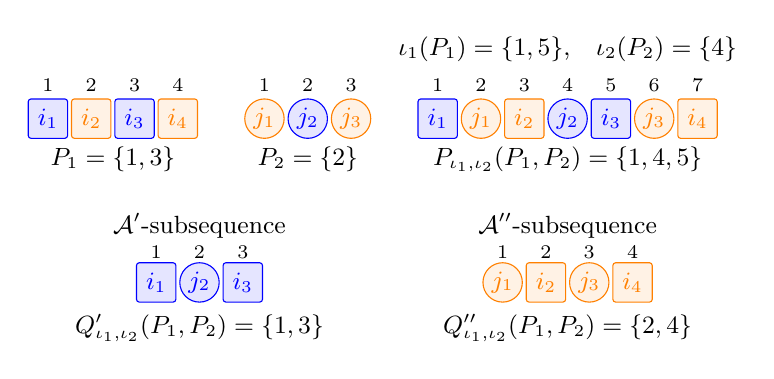
\begin{tikzpicture}[
        x=0.55cm,
        y=0.80cm,
        every node/.style={font=\small},
        firstword/.style={
            draw,
            rounded corners=1pt,
            minimum size=5mm,
            inner sep=0pt
        },
        secondword/.style={
            draw,
            circle,
            minimum size=5mm,
            inner sep=0pt
        }
    ]
        % Row 1 spans x=1..16, overall center x=8.5
        % First word: x=1..4, center=2.5
        \node[firstword, draw=blue, fill=blue!10]
            at (1,2.0) {$\blue{i_1}$};
        \node[firstword, draw=orange, fill=orange!10]
            at (2,2.0) {$\orange{i_2}$};
        \node[firstword, draw=blue, fill=blue!10]
            at (3,2.0) {$\blue{i_3}$};
        \node[firstword, draw=orange, fill=orange!10]
            at (4,2.0) {$\orange{i_4}$};

        \foreach \k in {1,...,4}
            \node at (\k,2.53) {\scriptsize \k};

        \node at (2.5,1.35) {$P_1=\{1,3\}$};

        % Second word: x=6..8, center=7
        \node[secondword, draw=orange, fill=orange!10]
            at (6,2.0) {$\orange{j_1}$};
        \node[secondword, draw=blue, fill=blue!10]
            at (7,2.0) {$\blue{j_2}$};
        \node[secondword, draw=orange, fill=orange!10]
            at (8,2.0) {$\orange{j_3}$};

        \foreach \k/\x in {1/6,2/7,3/8}
            \node at (\x,2.53) {\scriptsize \k};

        \node at (7,1.35) {$P_2=\{2\}$};

        % Shuffled word: x=10..16, center=13
        \node at (13,3.10)
            {$\iota_1(P_1) = \{1, 5\}$,\quad $\iota_2(P_2) = \{4\}$};

        \node[firstword, draw=blue, fill=blue!10]
            at (10,2.0) {$\blue{i_1}$};
        \node[secondword, draw=orange, fill=orange!10]
            at (11,2.0) {$\orange{j_1}$};
        \node[firstword, draw=orange, fill=orange!10]
            at (12,2.0) {$\orange{i_2}$};
        \node[secondword, draw=blue, fill=blue!10]
            at (13,2.0) {$\blue{j_2}$};
        \node[firstword, draw=blue, fill=blue!10]
            at (14,2.0) {$\blue{i_3}$};
        \node[secondword, draw=orange, fill=orange!10]
            at (15,2.0) {$\orange{j_3}$};
        \node[firstword, draw=orange, fill=orange!10]
            at (16,2.0) {$\orange{i_4}$};

        \foreach \k/\x in {1/10,2/11,3/12,4/13,5/14,6/15,7/16}
            \node at (\x,2.53) {\scriptsize \k};

        \node at (13,1.35) {$P_{\iota_1,\iota_2}(P_1,P_2)=\{1,4,5\}$};

        % Row 2: shifted down by an extra 0.4
        \node at (4.5,0.30) {$\mathcal{A}^{\prime}$-subsequence};
        \node at (13,0.30) {$\mathcal{A}^{\prime\prime}$-subsequence};

        % A': 3 nodes centered at x=4.5
        \node[firstword, draw=blue, fill=blue!10]
            at (3.5,-0.60) {$\blue{i_1}$};
        \node[secondword, draw=blue, fill=blue!10]
            at (4.5,-0.60) {$\blue{j_2}$};
        \node[firstword, draw=blue, fill=blue!10]
            at (5.5,-0.60) {$\blue{i_3}$};

        \foreach \k/\x in {1/3.5,2/4.5,3/5.5}
            \node at (\x,-0.12) {\scriptsize \k};

        \node at (4.5,-1.32)
            {$Q^{\prime}_{\iota_1, \iota_2}(P_1,P_2)=\{1,3\}$};

        % A'': 4 nodes centered at x=13
        \node[secondword, draw=orange, fill=orange!10]
            at (11.5,-0.60) {$\orange{j_1}$};
        \node[firstword, draw=orange, fill=orange!10]
            at (12.5,-0.60) {$\orange{i_2}$};
        \node[secondword, draw=orange, fill=orange!10]
            at (13.5,-0.60) {$\orange{j_3}$};
        \node[firstword, draw=orange, fill=orange!10]
            at (14.5,-0.60) {$\orange{i_4}$};

        \foreach \k/\x in {1/11.5,2/12.5,3/13.5,4/14.5}
            \node at (\x,-0.12) {\scriptsize \k};

        \node at (13,-1.32)
            {$Q^{\prime\prime}_{\iota_1, \iota_2}(P_1,P_2)=\{2,4\}$};

    \end{tikzpicture}
    \caption{The input words have placements
$P_1=\{1,3\}$ and $P_2=\{2\}$, and are shuffled by
$\iota_1(1,2,3,4)=(1,3,5,7)$ and
$\iota_2(1,2,3)=(2,4,6)$. The resulting shuffled output word has the
placement
$P_{\iota_1,\iota_2}(P_1,P_2)=\{1,4,5\}$ and induced subsequence
placements
$Q^{\prime}_{\iota_1,\iota_2}(P_1,P_2)=\{1,3\}$ and
$Q^{\prime\prime}_{\iota_1,\iota_2}(P_1,P_2)=\{2,4\}$.
Squares and circles distinguish letters from the input words, while blue and
orange distinguish $\mathcal{A}^{\prime}$- and
$\mathcal{A}^{\prime\prime}$-letters. The three output placements determine $(\iota_1,\iota_2)$ uniquely; in the shuffle precomputation, we therefore iterate over compatible triples of output placements.}\label{fig:ordered_shuffle_placements}
\end{figure}
We then represent the shuffle product by grouping the shuffles according to
the induced subsequence placements $Q^{\prime}$ and
$Q^{\prime\prime}$ and summing the corresponding output placements.
For
$Q^{\prime}\in\operatorname{Pl}(n_1,n_2)$ and
$Q^{\prime\prime}\in\operatorname{Pl}(m_1,m_2)$, define
\[
    S^{Q^{\prime},Q^{\prime\prime}}_{n_1,m_1,n_2,m_2}
    \colon
    \mathbb{R}^{|\operatorname{Pl}(n_1,m_1)|}
    \otimes
    \mathbb{R}^{|\operatorname{Pl}(n_2,m_2)|}
    \longrightarrow
    \mathbb{R}^{|\operatorname{Pl}(n,m)|}
\]
on basis elements by
\[
\begin{aligned}
    &
    S^{Q^{\prime},Q^{\prime\prime}}_{n_1,m_1,n_2,m_2}
    \left(
        e_{\operatorname{rk}(P_1)}
        \otimes
        e_{\operatorname{rk}(P_2)}
    \right) :=
    \sum_{\substack{
        (\iota_1,\iota_2)
        \in
        \operatorname{Sh}(n_1+m_1,n_2+m_2)\\
        Q^{\prime}_{\iota_1,\iota_2}(P_1,P_2)=Q^{\prime}\\
        Q^{\prime\prime}_{\iota_1,\iota_2}(P_1,P_2)=Q^{\prime\prime}
    }}
    e_{\operatorname{rk}
        \left(
            P_{\iota_1,\iota_2}(P_1,P_2)
        \right)}.
\end{aligned}
\]
The remaining part of the shuffle operation is then described by a
permutation of the dense axes. Let
$\Theta_{Q^{\prime},Q^{\prime\prime}}$ be the canonical permutation from
\[
    \mathbb{R}^{|\operatorname{Pl}(n_1,m_1)|}
    \otimes
    \left(
        \mathbb{R}^{|\mathcal{A}^{\prime}|}
    \right)^{\otimes n_1}
    \otimes
    \left(
        \mathbb{R}^{|\mathcal{A}^{\prime\prime}|}
    \right)^{\otimes m_1}
    \otimes
    \mathbb{R}^{|\operatorname{Pl}(n_2,m_2)|}
    \otimes
    \left(
        \mathbb{R}^{|\mathcal{A}^{\prime}|}
    \right)^{\otimes n_2}
    \otimes
    \left(
        \mathbb{R}^{|\mathcal{A}^{\prime\prime}|}
    \right)^{\otimes m_2}
\]
to
\[
    \mathbb{R}^{|\operatorname{Pl}(n_1,m_1)|}
    \otimes
    \mathbb{R}^{|\operatorname{Pl}(n_2,m_2)|}
    \otimes
    \left(
        \mathbb{R}^{|\mathcal{A}^{\prime}|}
    \right)^{\otimes n}
    \otimes
    \left(
        \mathbb{R}^{|\mathcal{A}^{\prime\prime}|}
    \right)^{\otimes m}
\]
which moves the two placement axes to the front, places the
$\mathcal{A}^{\prime}$-axes of the first input in the positions
$Q^{\prime}$, and places its $\mathcal{A}^{\prime\prime}$-axes in the
positions $Q^{\prime\prime}$.
We write $\Theta^{\mathrm{dense}}_{Q^{\prime},Q^{\prime\prime}}$ for the
corresponding permutation of the dense axes alone, leaving any leading batch
axes fixed.

\begin{lemma}
\label{lem:ordered_shuffle}
For
$\ell_1,\ell_2\in
\mathbb{R}^{N,M}\langle\mathcal{A}\rangle$,
\[
    \bigl(
        \ell_1\shuffle_{N,M}\ell_2
    \bigr)^{(n,m)}
    =
    \sum_{\substack{
        n_1+n_2=n\\
        m_1+m_2=m
    }}
    \;
    \sum_{\substack{
        Q^{\prime}\in\operatorname{Pl}(n_1,n_2)\\
        Q^{\prime\prime}\in\operatorname{Pl}(m_1,m_2)
    }}
    \left(
        S^{Q^{\prime},Q^{\prime\prime}}_{n_1,m_1,n_2,m_2}
        \otimes
        \operatorname{id}
    \right)
    \Theta_{Q^{\prime},Q^{\prime\prime}}
    \left(
        \ell_1^{(n_1,m_1)}
        \otimes
        \ell_2^{(n_2,m_2)}
    \right).
\]
\end{lemma}

\begin{proof}
By bilinearity, it suffices to consider two basis words with placements
$P_1\in\operatorname{Pl}(n_1,m_1)$ and
$P_2\in\operatorname{Pl}(n_2,m_2)$. Each
$(\iota_1,\iota_2)\in
\operatorname{Sh}(n_1+m_1,n_2+m_2)$ contributes one shuffled word. Its
placement coordinate is $\operatorname{rk}
        \left(
            P_{\iota_1,\iota_2}(P_1,P_2)
        \right)$,
while its dense $\mathcal{A}^{\prime}$- and
$\mathcal{A}^{\prime\prime}$-axes are obtained by interleaving the dense
axes of the two inputs according to
$Q^{\prime}_{\iota_1,\iota_2}(P_1,P_2)$ and
$Q^{\prime\prime}_{\iota_1,\iota_2}(P_1,P_2)$, respectively.

Fix
$Q^{\prime}\in\operatorname{Pl}(n_1,n_2)$ and
$Q^{\prime\prime}\in\operatorname{Pl}(m_1,m_2)$.
The permutation $\Theta_{Q^{\prime},Q^{\prime\prime}}$ produces the
dense coordinate part of precisely those shuffle terms for which
\[
    Q^{\prime}_{\iota_1,\iota_2}(P_1,P_2)=Q^{\prime},
    \qquad
    Q^{\prime\prime}_{\iota_1,\iota_2}(P_1,P_2)=Q^{\prime\prime}.
\]
For the same terms,
$S^{Q^{\prime},Q^{\prime\prime}}_{n_1,m_1,n_2,m_2}$ sums the
corresponding output placement coordinates. Hence
\[
    \left(
        S^{Q^{\prime},Q^{\prime\prime}}_{n_1,m_1,n_2,m_2}
        \otimes
        \operatorname{id}
    \right)
    \Theta_{Q^{\prime},Q^{\prime\prime}}
\]
is exactly the sum of all shuffle terms having the fixed induced
placements $(Q^{\prime},Q^{\prime\prime})$.

Every shuffle pair assigns a single such pair of induced placements,
so summing over $Q^{\prime}$ and $Q^{\prime\prime}$ exhausts all shuffle
terms without omission or repetition. Finally, summing over all
decompositions $n=n_1+n_2$ and $m=m_1+m_2$ gives the
$(n,m)$-block of $\ell_1\shuffle_{N,M}\ell_2$.
\end{proof}

To justify this sparse formula, we first record that the output placement together with the induced placements uniquely determines the input placements and the shuffle.

\begin{lemma}
\label{lem:shuffle_pullback}
The map
\[
    \operatorname{Pl}(n_1,m_1)
    \times
    \operatorname{Pl}(n_2,m_2)
    \times
    \operatorname{Sh}(n_1+m_1,n_2+m_2)
    \longrightarrow
    \operatorname{Pl}(n,m)
    \times
    \operatorname{Pl}(n_1,n_2)
    \times
    \operatorname{Pl}(m_1,m_2),
\]
given by
\[
    (P_1,P_2,\iota_1,\iota_2)
    \longmapsto
    \left(
        P_{\iota_1,\iota_2}(P_1,P_2),
        Q'_{\iota_1,\iota_2}(P_1,P_2),
        Q''_{\iota_1,\iota_2}(P_1,P_2)
    \right),
\]
is a bijection. In particular, for fixed $Q'$ and $Q''$, every output
placement arises from a unique pair of input placements and a unique
shuffle. Consequently, every matrix coefficient of
$S^{Q',Q''}_{n_1,m_1,n_2,m_2}$ is either zero or one.
\end{lemma}

\begin{proof}
We construct the inverse map. Let
$P=\{p_1<\cdots<p_n\}\in\operatorname{Pl}(n,m)$, write
$P^{\mathsf c}=\{q_1<\cdots<q_m\}$, and fix
$Q'\in\operatorname{Pl}(n_1,n_2)$ and
$Q''\in\operatorname{Pl}(m_1,m_2)$. Define
\[
    I_1
    :=
    \{p_r:r\in Q'\}
    \cup
    \{q_s:s\in Q''\},
    \qquad
    I_2
    :=
    \{1,\ldots,n+m\}\setminus I_1.
\]
Since $|I_1|=n_1+m_1$ and $|I_2|=n_2+m_2$, there are unique strictly
increasing maps $\iota_1$ and $\iota_2$ with images $I_1$ and $I_2$.
Define
\[
    P_1:=\iota_1^{-1}(P),
    \qquad
    P_2:=\iota_2^{-1}(P).
\]
The set $P_1$ consists of the $n_1$ indices corresponding to
$\{p_r:r\in Q'\}$, while $P_2$ consists of the $n_2$ indices
corresponding to the remaining positions in $P$. Hence
$P_1\in\operatorname{Pl}(n_1,m_1)$ and
$P_2\in\operatorname{Pl}(n_2,m_2)$. By construction,
\[
    P_{\iota_1,\iota_2}(P_1,P_2)=P,
    \qquad
    Q'_{\iota_1,\iota_2}(P_1,P_2)=Q',
    \qquad
    Q''_{\iota_1,\iota_2}(P_1,P_2)=Q''.
\]
\end{proof}

For
$0\leq r'<|\operatorname{Pl}(n_1,n_2)|$ and
$0\leq r''<|\operatorname{Pl}(m_1,m_2)|$, let
\[
    \mathsf{S}^{r',r''}_{n_1,m_1,n_2,m_2}
    \subseteq
    \{0,\ldots,|\operatorname{Pl}(n_1,m_1)|-1\}
    \times
    \{0,\ldots,|\operatorname{Pl}(n_2,m_2)|-1\}
    \times
    \{0,\ldots,|\operatorname{Pl}(n,m)|-1\}
\]
be the set of all triples $(j_1,j_2,k)$ such that the input placements
of ranks $j_1$ and $j_2$ produce the output placement of rank $k$ with
induced placements $Q'=\operatorname{rk}^{-1}(r')$ and
$Q''=\operatorname{rk}^{-1}(r'')$. Equivalently,
\[
    S^{Q',Q''}_{n_1,m_1,n_2,m_2}
    \left(e_{j_1}\otimes e_{j_2}\right)
    =
    \sum_{\substack{
        0\leq k<|\operatorname{Pl}(n,m)|\\
        (j_1,j_2,k)\in
        \mathsf{S}^{r',r''}_{n_1,m_1,n_2,m_2}
    }}
    e_k.
\]
By \Cref{lem:shuffle_pullback}, no multiplicities are required. These
sets are enumerated by \Cref{alg:shuffle_placement_arrays}.

\begin{algorithm}[ht]
\caption{Placement-rank lists for the shuffle}
\label{alg:shuffle_placement_arrays}
\begin{algorithmic}[1]
\Require bidegrees $(n_1,m_1)$ and $(n_2,m_2)$
\Ensure the lists
$\mathsf{S}^{r',r''}_{n_1,m_1,n_2,m_2}$
\State $n\gets n_1+n_2$, $m\gets m_1+m_2$
\ForAll{$Q'\in\operatorname{Pl}(n_1,n_2)$
    with increasing rank $r'$}
    \ForAll{$Q''\in\operatorname{Pl}(m_1,m_2)$
        with increasing rank $r''$}
        \State
        $\mathsf{S}^{r',r''}_{n_1,m_1,n_2,m_2}\gets[\,]$
    \EndFor
\EndFor
\ForAll{$P=\{p_1<\cdots<p_n\}\in\operatorname{Pl}(n,m)$
    with increasing rank $k$}
    \State write
    $P^{\mathsf c}=\{q_1<\cdots<q_m\}$
    \ForAll{$Q'\in\operatorname{Pl}(n_1,n_2)$
        with increasing rank $r'$}
        \ForAll{$Q''\in\operatorname{Pl}(m_1,m_2)$
            with increasing rank $r''$}
            \State
            $I_1\gets
            \{p_r:r\in Q'\}
            \cup
            \{q_s:s\in Q''\}$
            \State
            $I_2\gets
            \{1,\ldots,n+m\}\setminus I_1$
            \State write
            $I_1=\{h_1<\cdots<h_{n_1+m_1}\}$ and
            $I_2=\{\bar h_1<\cdots<\bar h_{n_2+m_2}\}$
            \State
            $P_1\gets\{a:h_a\in P\}$
            \State
            $P_2\gets\{b:\bar h_b\in P\}$
            \State append
            $\bigl(
                \operatorname{rk}(P_1),
                \operatorname{rk}(P_2),
                k
            \bigr)$
            to
            $\mathsf{S}^{r',r''}_{n_1,m_1,n_2,m_2}$
        \EndFor
    \EndFor
\EndFor
\end{algorithmic}
\end{algorithm}

\begin{implrmk}
The nested placement loops in
\Cref{alg:shuffle_placement_arrays} are precomputation only. At runtime,
the loops are over the bidegree splittings and the keys $(r',r'')$; there
is no loop over output placement ranks. For one fixed key, write $J_1$ and
$J_2$ for the two stored input-rank columns. The complete update is
\begin{algorithmic}[1]
\State $\mathbf{V}\gets
    \operatorname{batchouter}
    \left(
        \ell_1^{(n_1,m_1)}[J_1],
        \ell_2^{(n_2,m_2)}[J_2]
    \right)$
\State $\mathbf{V}\gets
    \Theta^{\mathrm{dense}}_{Q',Q''}\mathbf{V}$
\State $\mathbf{c}^{(n,m)}\mathrel{+}=\mathbf{V}$
\end{algorithmic}
Here $\operatorname{batchouter}$ forms one outer product for every row of
the gathered rank axis. The rows are already in increasing output-rank
order, so the final addition is contiguous and no output-rank or
coefficient array is stored. If necessary, the rows may be processed in
contiguous batches without changing the computation.
\end{implrmk}

\subsubsection{Computing signatures.}
Let $z=(z^{\prime},z^{\prime\prime})
    \in
    \mathbb{R}^{|\mathcal{A}^{\prime}|}
    \oplus
    \mathbb{R}^{|\mathcal{A}^{\prime\prime}|}.$
The bidegree-truncated product
\[
    \mathbf{b}_0
    =
    \pi^{N,M}
    \bigl(
        \mathbf{a}\otimes\exp_{\otimes}(z)
    \bigr)
\]
is computed by the Horner recursion in
\Cref{alg:ordered_signature_horner}, directly on the stored bidegree
blocks. Set $\kappa_{n,0}:=0$ and, for $m>0$,
$\kappa_{n,m}:=|\operatorname{Pl}(n,m-1)|$.

\begin{algorithm}[ht]
\caption{Horner recursion in ordered standard coordinates}
\label{alg:ordered_signature_horner}
\begingroup
\algrenewcommand\algorithmiccomment[1]{\hfill\texttt{//}#1}
\begin{algorithmic}[1]
\Require
$\mathbf{a}\in T^{N,M}(\mathbb{R}^{d})$ and
$z=(z^{\prime},z^{\prime\prime})\in\mathbb{R}^{d}$
\Ensure
$\mathbf{b}_0
=
\pi^{N,M}\bigl(\mathbf{a}\otimes\exp_{\otimes}(z)\bigr)$
\State
$\mathbf{b}_{N+M}^{(0,0)}
\gets
\mathbf{a}^{(0,0)}$
\State
All other blocks of $\mathbf{b}_{N+M}$ are absent
\For{$q=N+M,\ldots,1$}
    \State
    $\mathbf{b}_{q-1}^{(0,0)}
    \gets
    \mathbf{a}^{(0,0)}$
    \ForAll{$(n,m)$ such that
        $0\leq n\leq N$,
        $0\leq m\leq M$, and
        $1\leq n+m\leq N+M-q+1$}
        \Comment{\texttt{(*)}}
        \State
        $\mathbf{b}_{q-1}^{(n,m)}
        \gets
        \mathbf{a}^{(n,m)}$
        \If{$m>0$}
            \For{$k=0,\ldots,\kappa_{n,m}-1$}
                \State
                $\displaystyle
                \bigl(\mathbf{b}_{q-1}^{(n,m)}\bigr)_k
                \gets
                \bigl(\mathbf{b}_{q-1}^{(n,m)}\bigr)_k
                +
                \frac{1}{q}
                \bigl(\mathbf{b}_{q}^{(n,m-1)}\bigr)_k
                \otimes z^{\prime\prime}$
            \EndFor
        \EndIf
        \If{$n>0$}
            \For{$k=0,\ldots,|\operatorname{Pl}(n-1,m)|-1$}
                \State
                $\displaystyle
                \bigl(\mathbf{b}_{q-1}^{(n,m)}\bigr)_{k+\kappa_{n,m}}
                \gets
                \bigl(\mathbf{b}_{q-1}^{(n,m)}\bigr)_{k+\kappa_{n,m}}
                +
                \frac{1}{q}
                \tau_{n-1,m,1,0}
                \left(
                    \bigl(\mathbf{b}_{q}^{(n-1,m)}\bigr)_k
                    \otimes z^{\prime}
                \right)$
            \EndFor
        \EndIf
    \EndFor
\EndFor
\State \Return $\mathbf{b}_0$
\Statex
\Statex \texttt{(*)} For fixed $q$, the active bidegrees may be traversed
in any order and
their computation may be parallelized.
\end{algorithmic}
\endgroup
\end{algorithm}

The outer loop over $q$ and the active bidegrees in
\Cref{alg:ordered_signature_horner} is common to all four signature
computations. With $\widehat{\otimes}$, $\odot$, or
$\widehat{\odot}$, only the fixed-bidegree formula for right multiplication
by $z$ changes. In each case, repeated substitution in the corresponding
unpruned recursion gives the appropriate tensor exponential through degree
$N+M$. Since right multiplication by $z$ raises the total degree by one,
discarding inactive blocks cannot change any block retained by
$\pi^{N,M}$. We use this product--Horner argument below without repeating
it.

\begin{implrmk}
The runtime loops over the Horner depth $q$ and the active bidegrees remain,
but the placement-rank loops in
\Cref{alg:ordered_signature_horner} are vectorized. For a fixed
$(q,n,m)$, the complete block update is
\begin{algorithmic}[1]
\State $\mathbf{b}_{q-1}^{(n,m)}
    \gets\mathbf{a}^{(n,m)}$
\If{$m>0$}
    \State $\mathbf{b}_{q-1}^{(n,m)}
        [0:\kappa_{n,m}]
        \mathrel{+}=
        q^{-1}\mathbf{b}_{q}^{(n,m-1)}
        \otimes z^{\prime\prime}$
\EndIf
\If{$n>0$}
    \State $\mathbf{b}_{q-1}^{(n,m)}
        [\kappa_{n,m}:|\operatorname{Pl}(n,m)|]
        \mathrel{+}=
        q^{-1}\tau_{n-1,m,1,0}
        \left(
            \mathbf{b}_{q}^{(n-1,m)}
            \otimes z^{\prime}
        \right)$
\EndIf
\end{algorithmic}
Both assignments act on contiguous rank ranges and are vectorized over all
rank and dense axes. The Horner update itself does not consult any placement
map, and only $\mathbf{b}_{q}$ and $\mathbf{b}_{q-1}$ are live numerical
states.
\end{implrmk}

If $Y$ is piecewise linear on
$s=t_0<\cdots<t_J=t$, with increments
$\Delta Y_j=Y_{t_{j-1},t_j}$, we set
$\mathbf{S}_0=e_{\emptyset}$ and apply the recursion successively for
\[
    \mathbf{S}_j
    =
    \pi^{N,M}
    \bigl(
        \mathbf{S}_{j-1}
        \otimes
        \exp_{\otimes}(\Delta Y_j)
    \bigr),
    \qquad
    j=1,\ldots,J.
\]
Chen's identity then gives
$\mathbf{S}_J
    =
    \pi^{N,M}\Sig{Y}_{s,t}$.
The same partitionwise assembly applies in the remaining three settings,
using the corresponding product and fixed-bidegree update described below.

\subsection{Partially symmetrized coordinates}

\subsubsection{Concatenation.}
For
$\boldsymbol{\alpha}
=
(\alpha_0,\ldots,\alpha_{n_1})
\in\operatorname{MPl}(n_1,m_1)$
and
$\boldsymbol{\beta}
=
(\beta_0,\ldots,\beta_{n_2})
\in\operatorname{MPl}(n_2,m_2)$,
define
\[
    \boldsymbol{\alpha}\dott\boldsymbol{\beta}
    :=
    \left(
        \alpha_0,\ldots,\alpha_{n_1-1},
        \alpha_{n_1}+\beta_0,
        \beta_1,\ldots,\beta_{n_2}
    \right)
    \in
    \operatorname{MPl}(n_1+n_2,m_1+m_2).
\]
This merges the two adjacent
$\mathcal{A}^{\prime\prime}$-blocks at the concatenation boundary.
For $n=n_1+n_2$ and $m=m_1+m_2$, define the linear map
\[
    \widehat{C}_{n_1,m_1,n_2,m_2}
    \colon
    \mathbb{R}^{|\operatorname{MPl}(n_1,m_1)|}
    \otimes
    \mathbb{R}^{|\operatorname{MPl}(n_2,m_2)|}
    \longrightarrow
    \mathbb{R}^{|\operatorname{MPl}(n,m)|}
\]
on basis elements by
\[
    \widehat{C}_{n_1,m_1,n_2,m_2}
    \left(
        e_{\operatorname{rk}_{\mathrm{sym}}(\boldsymbol{\alpha})}
        \otimes
        e_{\operatorname{rk}_{\mathrm{sym}}(\boldsymbol{\beta})}
    \right)
    :=
    e_{\operatorname{rk}_{\mathrm{sym}}
    \left(
        \boldsymbol{\alpha}\dott\boldsymbol{\beta}
    \right)}.
\]
Let $\widehat{\tau}_{n_1,m_1,n_2,m_2}$ be the canonical permutation of
tensor factors which sends
\[
    \mathbb{R}^{|\operatorname{MPl}(n_1,m_1)|}
    \otimes
    \left(
        \mathbb{R}^{|\mathcal{A}^{\prime}|}
    \right)^{\otimes n_1}
    \otimes
    \mathbb{R}^{|\operatorname{MPl}(n_2,m_2)|}
    \otimes
    \left(
        \mathbb{R}^{|\mathcal{A}^{\prime}|}
    \right)^{\otimes n_2}
\]
to
\[
    \mathbb{R}^{|\operatorname{MPl}(n_1,m_1)|}
    \otimes
    \mathbb{R}^{|\operatorname{MPl}(n_2,m_2)|}
    \otimes
    \left(
        \mathbb{R}^{|\mathcal{A}^{\prime}|}
    \right)^{\otimes n}.
\]

Then, in complete analogy with \Cref{lem:ordered_concatenation}, we obtain
the following block formula.

\begin{lemma}
\label{lem:symmetrized_concatenation}
For
$\widehat{\mathbf{a}},\widehat{\mathbf{b}}
\in\widehat{T}^{N,M}(\mathbb{R}^{d})$,
\[
    \bigl(
        \widehat{\mathbf{a}}
        \widehat{\otimes}_{N,M}
        \widehat{\mathbf{b}}
    \bigr)^{(n,m)}
    =
    \sum_{\substack{
        n_1+n_2=n\\
        m_1+m_2=m
    }}
    \left(
        \widehat{C}_{n_1,m_1,n_2,m_2}
        \otimes
        \operatorname{id}
    \right)
    \widehat{\tau}_{n_1,m_1,n_2,m_2}
    \left(
        \widehat{\mathbf{a}}^{(n_1,m_1)}
        \otimes
        \widehat{\mathbf{b}}^{(n_2,m_2)}
    \right).
\]
\end{lemma}

In contrast to the ordered case, the map from pairs of input ranks to
the target rank is generally not injective, since the merged boundary
block $\alpha_{n_1}+\beta_0$ does not retain how its entries were split
between the two inputs. Thus,
$\widehat{C}_{n_1,m_1,n_2,m_2}$ is a genuine sparse accumulation map
rather than an injective re-indexing. Moreover, unlike
\eqref{eq:concat_ord_rankdecomp}, the target rank does not decompose as
the first input rank plus an offset depending only on the second input.
The interaction of the two inputs is, however, confined to the boundary
blocks, and the rank arithmetic remains fully explicit.
Indeed, recall
from the definition of $\operatorname{rk}_{\mathrm{sym}}$ in
\eqref{eq:rk_sym} that, using the fixed order on
$\mathcal{A}^{\prime\prime}$, each
$\boldsymbol{\alpha}\in\operatorname{MPl}(n_1,m_1)$ is flattened
blockwise as
$(a_1,\ldots,a_{(n_1+1)|\mathcal{A}^{\prime\prime}|})$. We define
\[
    \operatorname{rk}^{\mathrm{pre}}(\boldsymbol{\alpha})
    :=
    \sum_{r=1}^{n_1|\mathcal{A}^{\prime\prime}|}
    \binom{
        r-1+\sum_{\ell=1}^{r}a_\ell
    }{r}.
\]
Thus, $\operatorname{rk}^{\mathrm{pre}}$ collects the first
$n_1|\mathcal{A}^{\prime\prime}|$ terms of
$\operatorname{rk}_{\mathrm{sym}}$.
Write
$\mathcal{A}^{\prime\prime}
=
\{\orange{i_1},\ldots,
\orange{i_{|\mathcal{A}^{\prime\prime}|}}\}$
in its fixed order. For
$\mu,\nu\in\mathbb{N}_0^{\mathcal{A}^{\prime\prime}}$ and
$q\in\mathbb{N}_0$, define
\[
    \operatorname{rk}^{\mathrm{bd}}_{n_1}(\mu,\nu,q)
    :=
    \sum_{u=1}^{|\mathcal{A}^{\prime\prime}|}
    \binom{
        n_1|\mathcal{A}^{\prime\prime}|
        +u-1+q
        +\sum_{v=1}^{u}
        \left(
            \mu_{\orange{i_v}}
            +
            \nu_{\orange{i_v}}
        \right)
    }{
        n_1|\mathcal{A}^{\prime\prime}|+u
    }.
\]
Likewise, if
$(b_1,\ldots,b_{(n_2+1)|\mathcal{A}^{\prime\prime}|})$
is the blockwise flattening of
$\boldsymbol{\beta}\in\operatorname{MPl}(n_2,m_2)$, define
\[
    \operatorname{rk}^{\mathrm{suf}}_{n_1,m_1}
    (\boldsymbol{\beta})
    :=
    \sum_{u=|\mathcal{A}^{\prime\prime}|+1}^{
        (n_2+1)|\mathcal{A}^{\prime\prime}|
    }
    \binom{
        n_1|\mathcal{A}^{\prime\prime}|
        +u-1+m_1+\sum_{\ell=1}^{u}b_\ell
    }{
        n_1|\mathcal{A}^{\prime\prime}|+u
    }.
\]

\begin{lemma}
\label{lem:rk_sym_concat}
For $n=n_1+n_2$, $m=m_1+m_2$,
$\boldsymbol{\alpha}\in\operatorname{MPl}(n_1,m_1)$, and
$\boldsymbol{\beta}\in\operatorname{MPl}(n_2,m_2)$, we have
\[
\begin{aligned}
    \operatorname{rk}_{\mathrm{sym}}
    \left(
        \boldsymbol{\alpha}\dott\boldsymbol{\beta}
    \right)
    ={}&
    \operatorname{rk}^{\mathrm{pre}}(\boldsymbol{\alpha})
    +
    \operatorname{rk}^{\mathrm{bd}}_{n_1}
    \left(
        \alpha_{n_1},
        \beta_0,
        m_1-|\alpha_{n_1}|
    \right)
    +
    \operatorname{rk}^{\mathrm{suf}}_{n_1,m_1}
    (\boldsymbol{\beta})
    -
    \binom{
        (n+1)|\mathcal{A}^{\prime\prime}|-1+m
    }{
        (n+1)|\mathcal{A}^{\prime\prime}|
    }.
\end{aligned}
\]
\end{lemma}

\begin{proof}
Let
$(g_1,\ldots,g_{(n+1)|\mathcal{A}^{\prime\prime}|})$
be the flattening of
$\boldsymbol{\alpha}\dott\boldsymbol{\beta}$ and set
$S_r:=\sum_{\ell=1}^{r}g_\ell$.
For $r\leq n_1|\mathcal{A}^{\prime\prime}|$, the flattening agrees with
that of $\boldsymbol{\alpha}$, so
$S_r=\sum_{\ell=1}^{r}a_\ell$.
For
$r=n_1|\mathcal{A}^{\prime\prime}|+u$ with
$1\leq u\leq|\mathcal{A}^{\prime\prime}|$, the partial sum consists of
the weight of the prefix of $\boldsymbol{\alpha}$ and the first $u$
entries of the merged boundary block, so
\[
    S_r
    =
    m_1-|\alpha_{n_1}|
    +
    \sum_{v=1}^{u}
    \left(
        \alpha_{n_1,\orange{i_v}}
        +
        \beta_{0,\orange{i_v}}
    \right).
\]
For
$r=n_1|\mathcal{A}^{\prime\prime}|+u$ with
$|\mathcal{A}^{\prime\prime}|<u
\leq(n_2+1)|\mathcal{A}^{\prime\prime}|$, the partial sum contains the
full weight $m_1$ of $\boldsymbol{\alpha}$ and the first $u$ entries of
the flattening of $\boldsymbol{\beta}$, so
$S_r=m_1+\sum_{\ell=1}^{u}b_\ell$.
Summing $\binom{r-1+S_r}{r}$ over the three regions yields the three
terms on the right-hand side. Together, these regions cover
$r=1,\ldots,(n+1)|\mathcal{A}^{\prime\prime}|$, whereas
$\operatorname{rk}_{\mathrm{sym}}$ omits the final determined index
$r=(n+1)|\mathcal{A}^{\prime\prime}|$. Since
$S_{(n+1)|\mathcal{A}^{\prime\prime}|}=m$, its contribution gives the final subtraction.
\end{proof}
\begin{implrmk}
The outer loop over the bidegree splittings remains. For one fixed
splitting, all input-rank pairs and all dense axes are vectorized. Store only
the target-rank array
\[
    K(j_1,j_2)
    :=
    \operatorname{rk}_{\mathrm{sym}}
    \left(
        \boldsymbol{\alpha}\dott\boldsymbol{\beta}
    \right)
\]
in lexicographic input-pair order. The runtime update is
\begin{algorithmic}[1]
\State $\mathbf{V}\gets
    \widehat{\tau}_{n_1,m_1,n_2,m_2}
    \left(
        \widehat{\mathbf{a}}^{(n_1,m_1)}
        \otimes
        \widehat{\mathbf{b}}^{(n_2,m_2)}
    \right)$
\State flatten the two rank axes of $\mathbf{V}$
\State $\widehat{\mathbf{c}}^{(n,m)}\gets
    \operatorname{scatteradd}
    \left(
        \widehat{\mathbf{c}}^{(n,m)},K,\mathbf{V}
    \right)$
\end{algorithmic}
Here $\operatorname{scatteradd}(\mathbf{C},K,\mathbf{V})$ adds row $j$ of
$\mathbf{V}$ to row $K_j$ of $\mathbf{C}$, so repeated target ranks are
accumulated directly. Thus there is no runtime loop over $(j_1,j_2)$ and no
stored ordering, segment offsets, or list of distinct targets. If the pair
axis is too large to materialize, it may be processed in batches with partial
updates scattered to the same target ranks.
\end{implrmk}

\subsubsection{Shuffle.}
Although the quotient shuffle product
$\widehat{\shuffle}_{N,M}$ can be computed recursively in the partially
symmetrized block layout, we do not compile this recursion
directly in partially symmetrized standard coordinates. Already for
$\orange{i}\in\mathcal{A}^{\prime\prime}$ and
$\blue{k},\blue{\ell}\in\mathcal{A}^{\prime}$, we have
\[
\begin{aligned}
    \bigl([\orange{i}]\blue{k}\bigr)
    \widehat{\shuffle}
    \bigl([\orange{i}]\blue{\ell}\bigr)
    ={}&
    [\orange{i}]\blue{k}[\orange{i}]\blue{\ell}
    +
    2[\orange{i}\orange{i}]\blue{k}\blue{\ell}
    +
    2[\orange{i}\orange{i}]\blue{\ell}\blue{k}
    +
    [\orange{i}]\blue{\ell}[\orange{i}]\blue{k}.
\end{aligned}
\]
The coefficients arise because different shuffle placements produce the
same partially symmetrized basis element. In higher bidegrees, the
$\mathcal{A}^{\prime\prime}$-blocks may additionally split across several
gaps created by an interleaving of the
$\mathcal{A}^{\prime}$-skeletons, and all decompositions producing the
same output basis element must be accumulated.

By contrast, the corresponding product in partially symmetrized shear
coordinates is simply
\[
    \bigl([\orange{i}]\blue{k}\bigr)
    \gammashufflesym
    \bigl([\orange{i}]\blue{\ell}\bigr)
    =
    [\orange{i}]\blue{k}[\orange{i}]\blue{\ell}
    +
    [\orange{i}]\blue{\ell}[\orange{i}]\blue{k}.
\]
Indeed, $\gammashufflesym$ only interleaves the two units
$[\orange{i}]\blue{k}$ and
$[\orange{i}]\blue{\ell}$; no
$\mathcal{A}^{\prime\prime}$-block is split. More generally, only the
$\mathcal{A}^{\prime}$-skeletons are interleaved, while the two terminal
$\mathcal{A}^{\prime\prime}$-blocks are merged with a single
multi-binomial coefficient, as shown in
\Cref{lem:gamma_shuffle_sym}.

This suggests carrying out the entire computation on the dual side in
partially symmetrized shear coordinates. Under the coordinate
transformation, the dual coordinate map
$(\widehat{\Psi}^{-1})^{\ast}$ is characterized by
$\langle(\widehat{\Psi}^{-1})^{\ast}(\ell),\widehat{\mathbf{a}}\rangle
:=\langle\ell,\widehat{\Psi}^{-1}(\widehat{\mathbf{a}})\rangle$. Shuffle
products then satisfy
\[
    (\widehat{\Psi}^{-1})^{\ast}
    \left(
        \ell_1\widehat{\shuffle}_{N,M}\ell_2
    \right)
    =
    (\widehat{\Psi}^{-1})^{\ast}(\ell_1)
    \gammashufflesym_{N,M}
    (\widehat{\Psi}^{-1})^{\ast}(\ell_2),
\]
while right concatenation by
$\blue{i}\in\mathcal{A}^{\prime}$ is preserved\footnote{Right concatenation by
$\orange{i}\in\mathcal{A}^{\prime\prime}$, corresponding to integration
against $X^i$, must instead be transported to shear coordinates by
integration by parts
$(\widehat{\Psi}^{-1})^{\ast}\circ\mathcal{R}_{\orange{i}}\circ
\widehat{\Psi}^{\ast}$, where
$\mathcal{R}_{\orange{i}}(\ell)=\ell\orange{i}$.}:
\[
    (\widehat{\Psi}^{-1})^{\ast}(\ell\blue{i})
    =
    (\widehat{\Psi}^{-1})^{\ast}(\ell)\blue{i}.
\]


\subsubsection{Computing signatures.}
Let
$z=(z^{\prime},z^{\prime\prime})
\in
\mathbb{R}^{|\mathcal{A}^{\prime}|}
\oplus
\mathbb{R}^{|\mathcal{A}^{\prime\prime}|}$.
In direct analogy with the ordered-coordinate recursion in
\Cref{alg:ordered_signature_horner}, write
$\exp_{\widehat{\otimes}}(z):=\widehat{\exp_{\otimes}(z)}$. The
bidegree-truncated product
\[
    \widehat{\mathbf{b}}_0
    =
    \widehat{\mathbf{a}}
    \widehat{\otimes}_{N,M}
    \exp_{\widehat{\otimes}}(z)
\]
is computed by the outer recursion of
\Cref{alg:ordered_signature_horner}, with $\widehat{\otimes}$ in place of
$\otimes$ and the partially symmetrized fixed-bidegree update below.

\begin{implrmk}
The runtime loops over $q$ and the active bidegrees remain. For the
$z^{\prime\prime}$-contribution, vectorize jointly over
$\orange{i}\in\mathcal{A}^{\prime\prime}$, the complete input-rank axis,
and all dense $\mathcal{A}^{\prime}$-axes. Let
$\delta_{\orange{i}}\in\mathbb{N}_0^{\mathcal{A}^{\prime\prime}}$ be the
unit multi-index at $\orange{i}$. If
$(\alpha_0,\ldots,\alpha_n)
=\operatorname{rk}_{\mathrm{sym}}^{-1}(k)
\in\operatorname{MPl}(n,m-1)$, precompute
\[
    K^{\prime\prime}_{n,m}(\orange{i},k)
    :=
    \operatorname{rk}_{\mathrm{sym}}
    \left(
        \alpha_0,\ldots,
        \alpha_n+\delta_{\orange{i}}
    \right).
\]
Flatten the pairs $(\orange{i},k)$ in lexicographic order. The direct plan
stores the resulting target array $K^{\prime\prime}_{n,m}$. For the
destination-ordered plan, store the increasing array $H$ of distinct target
ranks, one primary edge index in $E_{\mathrm{pri}}$ for each entry of $H$,
and the remaining edge indices and targets in $E_{\mathrm{col}}$ and
$K_{\mathrm{col}}$. The fixed-bidegree update is
\begin{algorithmic}[1]
\State $\widehat{\mathbf{b}}_{q-1}^{(n,m)}
    \gets\widehat{\mathbf{a}}^{(n,m)}$
\If{$m>0$}
    \State form the flattened edge array
    $\mathbf{V}_{(\orange{i},k)}
    \gets
    q^{-1}z^{\prime\prime}_{\orange{i}}
    (\widehat{\mathbf{b}}_q^{(n,m-1)})_k$
    \If{the direct plan is retained}
        \State $\widehat{\mathbf{b}}_{q-1}^{(n,m)}
        \gets
        \operatorname{scatteradd}
        (\widehat{\mathbf{b}}_{q-1}^{(n,m)},
        K^{\prime\prime}_{n,m},\mathbf{V})$
    \Else
        \State $\widehat{\mathbf{b}}_{q-1}^{(n,m)}[H]
        \mathrel{+}=\mathbf{V}[E_{\mathrm{pri}}]$
        \State $\widehat{\mathbf{b}}_{q-1}^{(n,m)}
        \gets
        \operatorname{scatteradd}
        (\widehat{\mathbf{b}}_{q-1}^{(n,m)},
        K_{\mathrm{col}},\mathbf{V}[E_{\mathrm{col}}])$
    \EndIf
\EndIf
\If{$n>0$}
    \State $\widehat{\mathbf{b}}_{q-1}^{(n,m)}
        [|\operatorname{MPl}(n,m)|-|\operatorname{MPl}(n-1,m)|:
        |\operatorname{MPl}(n,m)|]
        \mathrel{+}=
        q^{-1}\widehat{\mathbf{b}}_{q}^{(n-1,m)}
        \otimes z^{\prime}$
\EndIf
\end{algorithmic}
There is no runtime loop over letters or multiset-placement ranks. The
direct plan retains only $K^{\prime\prime}_{n,m}$; the destination-ordered
plan retains $H$, $E_{\mathrm{pri}}$, $E_{\mathrm{col}}$, and
$K_{\mathrm{col}}$. Only two Horner states are live.
\end{implrmk}


\section{Operations in shear coordinates}
\label{sec:shear_coordinate_computation}

In this section, we express the coordinate transformations, transported
concatenation products, signature computations, and dual products. Since
$\Psi$ and $\Psi^{-1}$ are graded, they commute with $\pi_K$ and restrict to
$T^K(\mathbb{R}^d)$. Hence, under total-degree truncation, computations in
ordered shear coordinates are performed directly on the canonical dense
homogeneous components and require neither bidegree blocks nor placement
ranks. More precisely, enumerate the words of length $r$ as
$w_0,\ldots,w_{d^r-1}$ in the lexicographic order induced by the fixed
alphabet order and, for $L\in\{\Psi,\Psi^{-1}\}$, precompute
\[
    D_r^L(k,\ell)
    :=
    \big\langle
        w_k,
        L(e_{w_\ell})
    \big\rangle.
\]
If $x_\ell=\langle w_\ell,\mathbf{a}^{(r)}\rangle$, then the flattened
coefficient vector of $L(\mathbf{a}^{(r)})$ is $D_r^Lx$ and is reshaped
back to the canonical $r$-axis array. The nonzero row, column, and
coefficient lists of $D_r^L$ may be retained instead of the dense matrix
when this uses less memory. A finite maximum degree is required because
these degreewise maps are precomputed. The remainder of the section gives
the corresponding formulas in the bidegree block layouts of
\Cref{sec:placement_layouts}. As in
\Cref{sec:standard_coordinate_operations}, we first treat the ordered
coordinates and then their partially symmetrized counterparts.

\subsection{Ordered coordinates}


\subsubsection{Concatenation.}\label{sec:shear_concat}
Since $\Psi$ and $\Psi^{-1}$ preserve bidegrees, the transported product
from \Cref{sec:coordinate_changes_and_products} restricts to
\[
    \mathbf{a}\odot_{N,M}\mathbf{b}
    =
    \Psi
    \left(
        \Psi^{-1}(\mathbf{a})
        \otimes_{N,M}
        \Psi^{-1}(\mathbf{b})
    \right),
    \qquad
    \mathbf{a},\mathbf{b}
    \in
    T^{N,M}(\mathbb{R}^d).
\]


\subsubsection{Shuffle.}
Since $\gammashuffle$ adds bidegrees, it induces a truncated product
\[
    \gammashuffle_{N,M}
    :
    \mathbb{R}^{N,M}\langle\mathcal{A}\rangle
    \times
    \mathbb{R}^{N,M}\langle\mathcal{A}\rangle
    \longrightarrow
    \mathbb{R}^{N,M}\langle\mathcal{A}\rangle.
\]
Recall from \cite[Proposition~3.7]{mainpaper} that, for
$w,v\in\mathcal{W}_{\mathcal{A}}$,
$r,q\in\mathcal{W}_{\mathcal{A}^{\prime\prime}}$, and
$\blue{i},\blue{j}\in\mathcal{A}^{\prime}$, the product is recursively
determined by
\begin{equation}
\label{eq:gamma_shuf_recursion}
\left\{
\begin{aligned}
    r\gammashuffle q
    &=
    r\shuffle q,
    \\
    (w\blue{i}r)\gammashuffle q
    &=
    w\blue{i}(r\shuffle q),
    \\
    r\gammashuffle(v\blue{j}q)
    &=
    v\blue{j}(r\shuffle q),
    \\
    (w\blue{i}r)\gammashuffle(v\blue{j}q)
    &=
    \bigl(
        (w\blue{i})\gammashuffle v
    \bigr)
    \blue{j}(r\shuffle q)
    +
    \bigl(
        w\gammashuffle(v\blue{j})
    \bigr)
    \blue{i}(r\shuffle q).
\end{aligned}
\right.
\end{equation}
We now express the product in the ordered block layout. Fix bidegrees
$(n_1,m_1)$ and $(n_2,m_2)$, and write $n=n_1+n_2$ and
$m=m_1+m_2$. We identify two input placements
$P_1\in\operatorname{Pl}(n_1,m_1)$ and
$P_2\in\operatorname{Pl}(n_2,m_2)$ by their corresponding
$\mathcal{A}^{\prime\prime}$-block lengths
$\delta p_{l,1},\ldots,\delta p_{l,n_l+1}$, characterized by
\[
    P_l\cup\{n_l+m_l+1\}
    =
    \left\{
        t+\sum_{s=1}^{t}\delta p_{l,s}
        :
        t=1,\ldots,n_l+1
    \right\},
    \qquad
    l\in\{1,2\}.
\]
To interleave the two ordered sequences of
$\mathcal{A}^{\prime\prime}$-block/$\mathcal{A}^{\prime}$-letter units,
let
\[
    Q^{\prime}
    =
    \{q_1<\cdots<q_{n_1}\}
    \in
    \operatorname{Pl}(n_1,n_2),
\]
and write
\[
    \{\bar q_1<\cdots<\bar q_{n_2}\}
    =
    \{1,\ldots,n\}\setminus Q^{\prime}.
\]
The placement $Q^{\prime}$ specifies the order of the two sequences of
$\mathcal{A}^{\prime}$-letters. Define the merged block lengths
$\delta p_1,\ldots,\delta p_n$ by
\[
    \delta p_{q_s}
    =
    \delta p_{1,s},
    \qquad
    1\leq s\leq n_1,
    \qquad
    \delta p_{\bar q_t}
    =
    \delta p_{2,t},
    \qquad
    1\leq t\leq n_2.
\]
The resulting output placement is
\[
    P_{Q^{\prime}}(P_1,P_2)
    =
    \left\{
        t+\sum_{u=1}^{t}\delta p_u
        :
        t=1,\ldots,n
    \right\}
    \in
    \operatorname{Pl}(n,m).
\]
It remains to shuffle the two terminal
$\mathcal{A}^{\prime\prime}$-blocks. For
\[
    R
    \in
    \operatorname{Pl}
    \left(
        \delta p_{1,n_1+1},
        \delta p_{2,n_2+1}
    \right),
\]
define
\[
\begin{aligned}
    Q^{\prime\prime}_{Q^{\prime},R}(P_1,P_2)
    =
    &
    \bigcup_{s=1}^{n_1}
    \left(
        \sum_{u=1}^{q_s-1}\delta p_u
        +
        \{1,\ldots,\delta p_{1,s}\}
    \right)
    \\
    &\qquad
    \cup
    \left(
        \sum_{u=1}^{n}\delta p_u
        +
        R
    \right)
    \in
    \operatorname{Pl}(m_1,m_2),
\end{aligned}
\]
where $c+A=\{c+a:a\in A\}$ and
$\{1,\ldots,0\}=\emptyset$. Thus,
$Q^{\prime\prime}_{Q^{\prime},R}(P_1,P_2)$ records the positions occupied
by the $\mathcal{A}^{\prime\prime}$-letters of the first input within the
$\mathcal{A}^{\prime\prime}$-subsequence of the output.

\begin{figure}[ht]
    \centering
    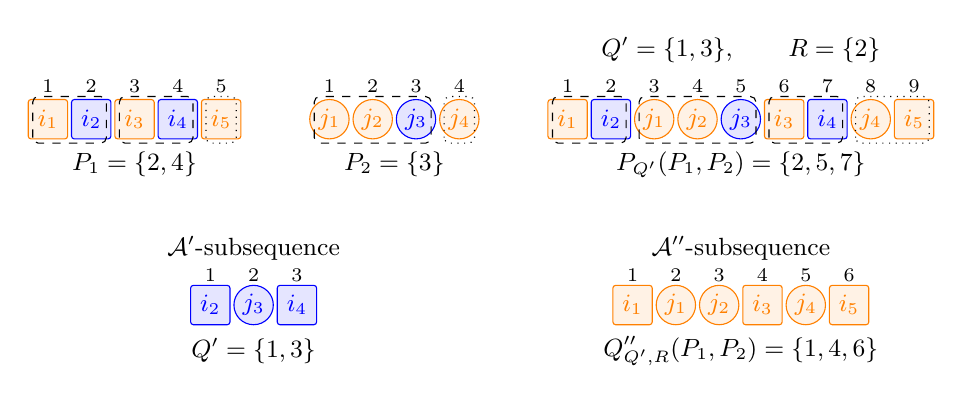
\begin{tikzpicture}[
        x=0.55cm,
        y=0.80cm,
        every node/.style={font=\small},
        firstword/.style={
            draw,
            rounded corners=1pt,
            minimum size=5mm,
            inner sep=0pt
        },
        secondword/.style={
            draw,
            circle,
            minimum size=5mm,
            inner sep=0pt
        }
    ]
        % Top row: the gaps between the three word groups are equal.

        % First input word: x=0,...,4, center x=2
        \node[firstword, draw=orange, fill=orange!10]
            at (0,2.0) {$\orange{i_1}$};
        \node[firstword, draw=blue, fill=blue!10]
            at (1,2.0) {$\blue{i_2}$};
        \node[firstword, draw=orange, fill=orange!10]
            at (2,2.0) {$\orange{i_3}$};
        \node[firstword, draw=blue, fill=blue!10]
            at (3,2.0) {$\blue{i_4}$};
        \node[firstword, draw=orange, fill=orange!10]
            at (4,2.0) {$\orange{i_5}$};

        \foreach \k/\x in {1/0,2/1,3/2,4/3,5/4}
            \node at (\x,2.53) {\scriptsize \k};

        \draw[dashed, rounded corners=2pt]
            (-0.35,1.62) rectangle (1.35,2.36);
        \draw[dashed, rounded corners=2pt]
            (1.65,1.62) rectangle (3.35,2.36);
        \draw[dotted, rounded corners=2pt]
            (3.65,1.62) rectangle (4.35,2.36);

        \node at (2,1.28) {$P_1=\{2,4\}$};

        % Second input word: x=6.5,...,9.5, center x=8
        \node[secondword, draw=orange, fill=orange!10]
            at (6.5,2.0) {$\orange{j_1}$};
        \node[secondword, draw=orange, fill=orange!10]
            at (7.5,2.0) {$\orange{j_2}$};
        \node[secondword, draw=blue, fill=blue!10]
            at (8.5,2.0) {$\blue{j_3}$};
        \node[secondword, draw=orange, fill=orange!10]
            at (9.5,2.0) {$\orange{j_4}$};

        \foreach \k/\x in {1/6.5,2/7.5,3/8.5,4/9.5}
            \node at (\x,2.53) {\scriptsize \k};

        \draw[dashed, rounded corners=2pt]
            (6.15,1.62) rectangle (8.85,2.36);
        \draw[dotted, rounded corners=2pt]
            (9.15,1.62) rectangle (9.85,2.36);

        \node at (8,1.28) {$P_2=\{3\}$};

        % Output word: x=12,...,20, center x=16
        \node at (16,3.10)
            {$Q^{\prime}=\{1,3\},\qquad R=\{2\}$};

        \node[firstword, draw=orange, fill=orange!10]
            at (12,2.0) {$\orange{i_1}$};
        \node[firstword, draw=blue, fill=blue!10]
            at (13,2.0) {$\blue{i_2}$};
        \node[secondword, draw=orange, fill=orange!10]
            at (14,2.0) {$\orange{j_1}$};
        \node[secondword, draw=orange, fill=orange!10]
            at (15,2.0) {$\orange{j_2}$};
        \node[secondword, draw=blue, fill=blue!10]
            at (16,2.0) {$\blue{j_3}$};
        \node[firstword, draw=orange, fill=orange!10]
            at (17,2.0) {$\orange{i_3}$};
        \node[firstword, draw=blue, fill=blue!10]
            at (18,2.0) {$\blue{i_4}$};
        \node[secondword, draw=orange, fill=orange!10]
            at (19,2.0) {$\orange{j_4}$};
        \node[firstword, draw=orange, fill=orange!10]
            at (20,2.0) {$\orange{i_5}$};

        \foreach \k/\x in {
            1/12,2/13,3/14,4/15,5/16,
            6/17,7/18,8/19,9/20
        }
            \node at (\x,2.53) {\scriptsize \k};

        \draw[dashed, rounded corners=2pt]
            (11.65,1.62) rectangle (13.35,2.36);
        \draw[dashed, rounded corners=2pt]
            (13.65,1.62) rectangle (16.35,2.36);
        \draw[dashed, rounded corners=2pt]
            (16.65,1.62) rectangle (18.35,2.36);
        \draw[dotted, rounded corners=2pt]
            (18.65,1.62) rectangle (20.35,2.36);

        \node at (16,1.28)
            {$P_{Q^{\prime}}(P_1,P_2)=\{2,5,7\}$};

        % Lower row: the first subsequence is centered below the two inputs,
        % and the second is centered below the output word.

        % A'-subsequence, center x=4.75
        \node at (4.75,-0.05)
            {$\mathcal{A}^{\prime}$-subsequence};

        \node[firstword, draw=blue, fill=blue!10]
            at (3.75,-0.95) {$\blue{i_2}$};
        \node[secondword, draw=blue, fill=blue!10]
            at (4.75,-0.95) {$\blue{j_3}$};
        \node[firstword, draw=blue, fill=blue!10]
            at (5.75,-0.95) {$\blue{i_4}$};

        \foreach \k/\x in {1/3.75,2/4.75,3/5.75}
            \node at (\x,-0.47) {\scriptsize \k};

        \node at (4.75,-1.68)
            {$Q^{\prime}=\{1,3\}$};

        % A''-subsequence, center x=16
        \node at (16,-0.05)
            {$\mathcal{A}^{\prime\prime}$-subsequence};

        \node[firstword, draw=orange, fill=orange!10]
            at (13.5,-0.95) {$\orange{i_1}$};
        \node[secondword, draw=orange, fill=orange!10]
            at (14.5,-0.95) {$\orange{j_1}$};
        \node[secondword, draw=orange, fill=orange!10]
            at (15.5,-0.95) {$\orange{j_2}$};
        \node[firstword, draw=orange, fill=orange!10]
            at (16.5,-0.95) {$\orange{i_3}$};
        \node[secondword, draw=orange, fill=orange!10]
            at (17.5,-0.95) {$\orange{j_4}$};
        \node[firstword, draw=orange, fill=orange!10]
            at (18.5,-0.95) {$\orange{i_5}$};

        \foreach \k/\x in {
            1/13.5,2/14.5,3/15.5,
            4/16.5,5/17.5,6/18.5
        }
            \node at (\x,-0.47) {\scriptsize \k};

        \node at (16,-1.68)
            {$Q^{\prime\prime}_{Q^{\prime},R}(P_1,P_2)
            =\{1,4,6\}$};
    \end{tikzpicture}
    \caption{The input words have placements
    $P_1=\{2,4\}$ and $P_2=\{3\}$. The placement
    $Q^{\prime}=\{1,3\}$ orders the two
    $\mathcal{A}^{\prime\prime}$-block/$\mathcal{A}^{\prime}$-letter
    units of the first input around the unit of the second input, while
    $R=\{2\}$ shuffles the two terminal
    $\mathcal{A}^{\prime\prime}$-blocks. The resulting output word has
    placement $P_{Q^{\prime}}(P_1,P_2)=\{2,5,7\}$, and the induced
    $\mathcal{A}^{\prime\prime}$-subsequence placement is
    $Q^{\prime\prime}_{Q^{\prime},R}(P_1,P_2)=\{1,4,6\}$.
    Squares and circles distinguish letters from the two input words,
    while blue and orange distinguish
    $\mathcal{A}^{\prime}$- and
    $\mathcal{A}^{\prime\prime}$-letters.}
    \label{fig:ordered_gamma_shuffle_placements}
\end{figure}

We represent $\gammashuffle_{N,M}$ by grouping its terms according to the
induced subsequence placements $Q^{\prime}$ and $Q^{\prime\prime}$ and
summing the corresponding output placements. For
$Q^{\prime}\in\operatorname{Pl}(n_1,n_2)$ and
$Q^{\prime\prime}\in\operatorname{Pl}(m_1,m_2)$, define
\[
    S^{\bullet,Q^{\prime},Q^{\prime\prime}}_{n_1,m_1,n_2,m_2}
    \colon
    \mathbb{R}^{|\operatorname{Pl}(n_1,m_1)|}
    \otimes
    \mathbb{R}^{|\operatorname{Pl}(n_2,m_2)|}
    \longrightarrow
    \mathbb{R}^{|\operatorname{Pl}(n,m)|}
\]
on basis elements by
\[
    S^{\bullet,Q^{\prime},Q^{\prime\prime}}_{n_1,m_1,n_2,m_2}
    \left(
        e_{\operatorname{rk}(P_1)}
        \otimes
        e_{\operatorname{rk}(P_2)}
    \right)
    =
    \sum_{\substack{
        R\in
        \operatorname{Pl}
        \left(
            \delta p_{1,n_1+1},
            \delta p_{2,n_2+1}
        \right)\\
        Q^{\prime\prime}_{Q^{\prime},R}(P_1,P_2)
        =
        Q^{\prime\prime}
    }}
    e_{\operatorname{rk}
        \left(
            P_{Q^{\prime}}(P_1,P_2)
        \right)}.
\]
The dense axes are permuted by the same canonical maps
$\Theta_{Q^{\prime},Q^{\prime\prime}}$ as in
\Cref{sec:ord_shuffle} for the ordered standard-coordinate shuffle.

\begin{lemma}
\label{lem:gamma_shuffle_units}
For
$\ell_1,\ell_2\in
\mathbb{R}^{N,M}\langle\mathcal{A}\rangle$,
\[
    \bigl(
        \ell_1\gammashuffle_{N,M}\ell_2
    \bigr)^{(n,m)}
    =
    \sum_{\substack{
        n_1+n_2=n\\
        m_1+m_2=m
    }}
    \;
    \sum_{\substack{
        Q^{\prime}\in\operatorname{Pl}(n_1,n_2)\\
        Q^{\prime\prime}\in\operatorname{Pl}(m_1,m_2)
    }}
    \left(
        S^{\bullet,Q^{\prime},Q^{\prime\prime}}_{n_1,m_1,n_2,m_2}
        \otimes
        \operatorname{id}
    \right)
    \Theta_{Q^{\prime},Q^{\prime\prime}}
    \left(
        \ell_1^{(n_1,m_1)}
        \otimes
        \ell_2^{(n_2,m_2)}
    \right).
\]
For each bidegree splitting, the inner sum is supported on
\[
    \Bigl\{
        \left(
            Q^{\prime},
            Q^{\prime\prime}_{Q^{\prime},R}(P_1,P_2)
        \right)
        :\;
        P_l\in\operatorname{Pl}(n_l,m_l),
        \;\; l\in\{1,2\},
        \;\;
        Q^{\prime}\in\operatorname{Pl}(n_1,n_2),
        \;\;
        R\in
        \operatorname{Pl}
        \left(
            \delta p_{1,n_1+1},
            \delta p_{2,n_2+1}
        \right)
    \Bigr\}.
\]
\end{lemma}

\begin{proof}
We use the notation introduced before the lemma. By bilinearity, it
suffices to consider two basis words with placements $P_1$ and $P_2$. In
the recursion \eqref{eq:gamma_shuf_recursion}, each
$\mathcal{A}^{\prime\prime}$-block preceding an
$\mathcal{A}^{\prime}$-letter remains attached to that letter. The two
ordered sequences of such units are therefore interleaved according to a
unique $Q^{\prime}\in\operatorname{Pl}(n_1,n_2)$. The merged block
lengths are $\delta p_1,\ldots,\delta p_n$, so the $t$-th
$\mathcal{A}^{\prime}$-letter occurs at position
$t+\sum_{u=1}^{t}\delta p_u$. This gives the output placement
$P_{Q^{\prime}}(P_1,P_2)$.

The recursion applies the ordinary shuffle only to the two terminal
$\mathcal{A}^{\prime\prime}$-blocks. Its terms are indexed by
\[
    R
    \in
    \operatorname{Pl}
    \left(
        \delta p_{1,n_1+1},
        \delta p_{2,n_2+1}
    \right),
\]
and the positions occupied by all
$\mathcal{A}^{\prime\prime}$-letters of the first input are precisely
$Q^{\prime\prime}_{Q^{\prime},R}(P_1,P_2)$. Hence, the dense axes of the
corresponding term are permuted by
\[
    \Theta_{
        Q^{\prime},
        Q^{\prime\prime}_{Q^{\prime},R}(P_1,P_2)
    }.
\]

Grouping the terms according to the resulting pair
$(Q^{\prime},Q^{\prime\prime})$ gives the displayed formula and
its stated support. The recursion partitions the unit interleavings
according to the final $\mathcal{A}^{\prime}$-letter, and the ordinary
terminal shuffle contains each $R$ once. Thus, for fixed input placements
$P_1$ and $P_2$, every pair $(Q^{\prime},R)$ contributes exactly once,
with coefficient one.
\end{proof}

As in the standard-coordinate shuffle, the output placement and the two
induced subsequence placements determine the input data uniquely.

\begin{lemma}
\label{lem:gamma_shuffle_pullback}
For fixed bidegrees, the map
\[
    \left(
        P_1,P_2,Q^{\prime},R
    \right)
    \longmapsto
    \left(
        P_{Q^{\prime}}(P_1,P_2),
        Q^{\prime},
        Q^{\prime\prime}_{Q^{\prime},R}(P_1,P_2)
    \right)
\]
is injective, where
$P_l\in\operatorname{Pl}(n_l,m_l)$,
$Q^{\prime}\in\operatorname{Pl}(n_1,n_2)$, and
\[
    R
    \in
    \operatorname{Pl}
    \left(
        \delta p_{1,n_1+1},
        \delta p_{2,n_2+1}
    \right).
\]
Consequently, every matrix coefficient of
$S^{\bullet,Q^{\prime},Q^{\prime\prime}}_{n_1,m_1,n_2,m_2}$
is either zero or one.
\end{lemma}

\begin{proof}
We reverse the construction above step by step. From
$P_{Q^{\prime}}(P_1,P_2)=\{p_1<\cdots<p_n\}$, with $p_0=0$, we recover
the merged block lengths as
\[
    \delta p_t
    =
    p_t-p_{t-1}-1,
    \qquad
    t=1,\ldots,n.
\]
The placement $Q^{\prime}=\{q_1<\cdots<q_{n_1}\}$ and its complement
$\{\bar q_1<\cdots<\bar q_{n_2}\}$ then recover the nonterminal block
lengths of the two inputs through
\[
    \delta p_{1,s}
    =
    \delta p_{q_s},
    \qquad
    \delta p_{2,t}
    =
    \delta p_{\bar q_t}.
\]
Their terminal block lengths follow from
\[
    \delta p_{l,n_l+1}
    =
    m_l-\sum_{s=1}^{n_l}\delta p_{l,s},
    \qquad
    l\in\{1,2\},
\]
and hence the defining block-length encoding recovers $P_1$ and
$P_2$. Finally, writing
$d=\sum_{u=1}^{n}\delta p_u$, we recover the terminal shuffle placement
from
\[
    R
    =
    \left(
        Q^{\prime\prime}_{Q^{\prime},R}(P_1,P_2)
        \cap
        \{d+1,\ldots,m\}
    \right)
    -
    d.
\]
Thus, the image determines $P_1$, $P_2$, $Q^{\prime}$, and $R$ uniquely,
which proves injectivity.
\end{proof}

For
$0\leq r'<|\operatorname{Pl}(n_1,n_2)|$ and
$0\leq r''<|\operatorname{Pl}(m_1,m_2)|$, define
\[
    \mathsf{S}^{\bullet,r',r''}_{n_1,m_1,n_2,m_2}
    \subseteq
    \{0,\ldots,|\operatorname{Pl}(n_1,m_1)|-1\}
    \times
    \{0,\ldots,|\operatorname{Pl}(n_2,m_2)|-1\}
    \times
    \{0,\ldots,|\operatorname{Pl}(n,m)|-1\}
\]
as the set of all triples
\[
    \left(
        \operatorname{rk}(P_1),
        \operatorname{rk}(P_2),
        \operatorname{rk}
        \left(
            P_{Q^{\prime}}(P_1,P_2)
        \right)
    \right)
\]
such that
\[
    Q^{\prime}
    =
    \operatorname{rk}^{-1}(r'),
    \qquad
    R
    \in
    \operatorname{Pl}
    \left(
        \delta p_{1,n_1+1},
        \delta p_{2,n_2+1}
    \right),
    \qquad
    \operatorname{rk}
    \left(
        Q^{\prime\prime}_{Q^{\prime},R}(P_1,P_2)
    \right)
    =
    r''.
\]
Equivalently, for
$Q^{\prime}=\operatorname{rk}^{-1}(r')$ and
$Q^{\prime\prime}=\operatorname{rk}^{-1}(r'')$,
\[
    S^{\bullet,Q^{\prime},Q^{\prime\prime}}_{n_1,m_1,n_2,m_2}
    \left(
        e_{j_1}\otimes e_{j_2}
    \right)
    =
    \sum_{\substack{
        0\leq k<|\operatorname{Pl}(n,m)|\\
        (j_1,j_2,k)\in
        \mathsf{S}^{\bullet,r',r''}_{n_1,m_1,n_2,m_2}
    }}
    e_k.
\]
By \Cref{lem:gamma_shuffle_pullback}, no multiplicities or coefficient
arrays are required. The lists are generated directly by enumerating
$P_1$, $P_2$, $Q^{\prime}$, and $R$ as described in the following
algorithm.

\begin{algorithm}[ht]
\caption{Placement-rank lists for the ordered shear shuffle}
\label{alg:gamma_shuffle_placement_arrays}
\begin{algorithmic}[1]
\Require bidegrees $(n_1,m_1)$ and $(n_2,m_2)$
\Ensure the nonempty lists
$\mathsf{S}^{\bullet,r',r''}_{n_1,m_1,n_2,m_2}$
\State $n\gets n_1+n_2$, $m\gets m_1+m_2$
\State initialize an empty associative collection of lists
\ForAll{$P_1\in\operatorname{Pl}(n_1,m_1)$
    with increasing rank $j_1$}
    \State compute
    $\delta p_{1,1},\ldots,\delta p_{1,n_1+1}$
    \ForAll{$P_2\in\operatorname{Pl}(n_2,m_2)$
        with increasing rank $j_2$}
        \State compute
        $\delta p_{2,1},\ldots,\delta p_{2,n_2+1}$
        \ForAll{$Q^{\prime}
            =\{q_1<\cdots<q_{n_1}\}
            \in\operatorname{Pl}(n_1,n_2)$
            with increasing rank $r'$}
            \State write
            $\{\bar q_1<\cdots<\bar q_{n_2}\}
            =
            \{1,\ldots,n\}\setminus Q^{\prime}$
            \State set
            $\delta p_{q_s}\gets\delta p_{1,s}$
            for $s=1,\ldots,n_1$
            \State set
            $\delta p_{\bar q_t}\gets\delta p_{2,t}$
            for $t=1,\ldots,n_2$
            \State
            $P\gets P_{Q^{\prime}}(P_1,P_2)$
            \State
            $k\gets\operatorname{rk}(P)$
            \ForAll{$R\in
                \operatorname{Pl}
                \left(
                    \delta p_{1,n_1+1},
                    \delta p_{2,n_2+1}
                \right)$
                with increasing rank}
                \State
                $Q^{\prime\prime}
                \gets
                Q^{\prime\prime}_{Q^{\prime},R}(P_1,P_2)$
                \State
                $r''\gets\operatorname{rk}(Q^{\prime\prime})$
                \If{the key $(r',r'')$ is absent}
                    \State initialize
                    $\mathsf{S}^{\bullet,r',r''}_{n_1,m_1,n_2,m_2}
                    \gets[\,]$
                \EndIf
                \State append $(j_1,j_2,k)$ to
                $\mathsf{S}^{\bullet,r',r''}_{n_1,m_1,n_2,m_2}$
            \EndFor
        \EndFor
    \EndFor
\EndFor
\State \Return the nonempty keyed lists
$\mathsf{S}^{\bullet,r',r''}_{n_1,m_1,n_2,m_2}$
\end{algorithmic}
\end{algorithm}

\begin{implrmk}
The nested loops in
\Cref{alg:gamma_shuffle_placement_arrays} are precomputation only. At
runtime, the loops are over the bidegree splittings and the nonempty keys
$(r',r'')$. For one key, write $(J_1,J_2,K)$ for the three stored rank
columns. The complete keyed update is
\begin{algorithmic}[1]
\State $\mathbf{V}\gets
    \operatorname{batchouter}
    \left(
        \ell_1^{(n_1,m_1)}[J_1],
        \ell_2^{(n_2,m_2)}[J_2]
    \right)$
\State $\mathbf{V}\gets
    \Theta^{\mathrm{dense}}_{Q',Q''}\mathbf{V}$
\State $\mathbf{c}^{(n,m)}[K]\mathrel{+}=\mathbf{V}$
\end{algorithmic}
By \Cref{lem:gamma_shuffle_pullback}, the entries of $K$ are distinct
within one key. Hence the final line is one vectorized indexed addition and
requires no reduction. There is no runtime loop over the stored triples;
if a keyed list is too large, it may be processed in contiguous batches.
Every term has coefficient one.
\end{implrmk}

\subsubsection{Coordinate transformations.}
\label{sec:transformations}

Recall from \Cref{sec:shear_coordinate_transformation} that $\Psi$ maps
standard coordinates to shear coordinates, while $\Psi^{-1}$ maps shear
coordinates back to standard coordinates. Both transformations preserve
bidegrees and the ordered sequence of
$\mathcal{A}^{\prime}$-letters. At a fixed bidegree $(n,m)$, they may
therefore change the placement of the
$\mathcal{A}^{\prime}$-letters and the order of the
$\mathcal{A}^{\prime\prime}$-letters, but not the order of the
$\mathcal{A}^{\prime}$-letters.

We first introduce the notation used to describe and store these actions.
For
$P\in\operatorname{Pl}(n,m)$ and
$k=\operatorname{rk}(P)$, recall from
\Cref{sec:placement_layouts} that
\(
    \mathbf{a}^{(n,m)}_k
    \in
    (
        \mathbb{R}^{|\mathcal{A}^{\prime}|}
    )^{\otimes n}
    \otimes
    (
        \mathbb{R}^{|\mathcal{A}^{\prime\prime}|}
    )^{\otimes m}
\)
is the placement slice containing the coefficients of the words whose
$\mathcal{A}^{\prime}$-letters occupy the positions $P$. We refer to
$\mathbf{a}^{(n,m)}_\ell$ as an input placement slice and to
$\bigl[\Psi^{\pm1}(\mathbf{a})^{(n,m)}\bigr]_k$ as an output placement
slice. Thus, an individual term in either transformation reads one input
placement slice, permutes its dense
$\mathcal{A}^{\prime\prime}$-axes, and adds the resulting tensor to one
output placement slice.

We use the following further notation: For tuples
$a=(a_1,\ldots,a_u)$ and
$b=(b_1,\ldots,b_v)$, we write
\[
    a\mathbin{\Vert}b
    :=
    (a_1,\ldots,a_u,b_1,\ldots,b_v)
\]
for their concatenation. Empty tuples and empty index ranges are omitted.
We identify a permutation
$\sigma\in\mathfrak{S}_m$ with its one-line notation
\[
    \sigma
    =
    (\sigma_1,\ldots,\sigma_m).
\]
It acts on the dense
$\mathcal{A}^{\prime\prime}$-axes of a placement slice by
\[
    \left[
        \bigl(
            \operatorname{id}^{\otimes n}
            \otimes\sigma
        \bigr)
        \mathbf{a}^{(n,m)}_\ell
    \right]_{
        i_1,\ldots,i_n,j_1,\ldots,j_m
    }
    =
    \left[
        \mathbf{a}^{(n,m)}_\ell
    \right]_{
        i_1,\ldots,i_n,
        j_{\sigma_1},\ldots,j_{\sigma_m}
    }.
\]
Thus the dense $\mathcal{A}^{\prime}$-axes are left fixed and only the
dense $\mathcal{A}^{\prime\prime}$-axes are permuted.
For constructing permutation tuples, given
\[
    Q=\{q_1<\cdots<q_u\}
    \in
    \operatorname{Pl}(u,v),\qquad \{\bar q_1<\cdots<\bar q_v\}
    =
    \{1,\ldots,u+v\}\setminus Q,
\]
and tuples
$a=(a_1,\ldots,a_u)$ and
$b=(b_1,\ldots,b_v)$, we define
\[
    \operatorname{merge}_{Q}(a,b)
    =
    (c_1,\ldots,c_{u+v}),
    \qquad
    c_{q_s}=a_s,
    \qquad
    c_{\bar q_t}=b_t.
\]
Thus $\operatorname{merge}_{Q}(a,b)$ interleaves the entries of $a$ and
$b$ while preserving their respective orders.

The permutation entries in all mathematical formulas are labelled by
$1,\ldots,m$. By contrast, placement ranks and the integer keys introduced
below are indexed from zero. Any conversion of a permutation tuple to the
zero-based axis convention of a particular tensor backend is an
implementation detail and is not included in the mathematical notation.

At fixed bidegree, we compute each output placement slice as a sparse sum
of input placement slices after permuting the dense
$\mathcal{A}^{\prime\prime}$-axes. By the \emph{support} of either
transformation at bidegree $(n,m)$, we mean the collection of its nonzero
contributions, each specified by an output placement, an input placement,
and a permutation of the dense
$\mathcal{A}^{\prime\prime}$-axes. For a graded linear map $L$ and a word
$w\in\mathcal{W}_{\mathcal{A}}$, we write $L_w$ for its graded row,
characterized by
$\langle w,L(\mathbf{a})\rangle=\langle L_w,\mathbf{a}\rangle$.
The graded-row identities established in
\cite[Propositions~3.2 and~3.7]{mainpaper} provide recursive descriptions
of these supports. For
$u\in\mathcal{W}_{\mathcal{A}^{\prime\prime}}$,
$w\in\mathcal{W}_{\mathcal{A}}$,
$\blue{i}\in\mathcal{A}^{\prime}$, and
$\orange{i_1},\ldots,\orange{i_r}
\in\mathcal{A}^{\prime\prime}$, these identities are
\begin{equation}
\label{eq:psi_row_recursion}
    \Psi_u
    =
    u,
    \qquad
    \Psi_{w\blue{i}u}
    =
    \bigl(
        \Psi_w\blue{i}
    \bigr)
    \shuffle u,
\end{equation}
and
\begin{equation}
\label{eq:psi_inverse_row_recursion}
    \Psi^{-1}_u
    =
    u,
    \qquad
    \Psi^{-1}_{w\blue{i}\orange{i_1}\cdots\orange{i_r}}
    =
    \sum_{q=0}^{r}
    (-1)^q
    \bigl(
        \Psi^{-1}_w
        \gammashuffle
        \orange{i_q}\cdots\orange{i_1}
    \bigr)
    \blue{i}
    \orange{i_{q+1}}\cdots\orange{i_r},
\end{equation}
where empty strings of letters are omitted.

We use the superscript $+$ for the support of $\Psi$ and the superscript
$-$ for the support of $\Psi^{-1}$. For each bidegree $(n,m)$, let
\[
    \Sigma^{\pm}_{n,m}
    =
    \bigl(
        \sigma^{\pm}_{n,m,c}
    \bigr)_{0\leq c<|\Sigma^{\pm}_{n,m}|}
\]
be the table of the distinct permutations that occur in the corresponding
transformation, indexed in order of first occurrence. During construction,
a dictionary assigns to each permutation tuple $\sigma$ its zero-based key
\[
    \operatorname{key}^{\pm}_{n,m}(\sigma)
    \in
    \{0,\ldots,|\Sigma^{\pm}_{n,m}|-1\}.
\]
If the tuple has already occurred, the dictionary returns its existing key;
otherwise, it appends the tuple to $\Sigma^{\pm}_{n,m}$ and returns the new
key.

We encode the sparse support by
\[
    \mathsf{T}^{\pm}_{n,m}
    \subseteq
    \{0,\ldots,|\operatorname{Pl}(n,m)|-1\}^{2}
    \times
    \{0,\ldots,|\Sigma^{\pm}_{n,m}|-1\}.
\]
An entry
\[
    (k,\ell,c)
    \in
    \mathsf{T}^{\pm}_{n,m}
\]
means that the input placement slice
$\mathbf{a}^{(n,m)}_\ell$, after permutation of its dense
$\mathcal{A}^{\prime\prime}$-axes by
$\sigma^{\pm}_{n,m,c}$, contributes to the output placement slice of rank
$k$.

For the recursive construction and the explicit formulas for the
transformations, it is convenient to group the support entries by their
output rank, since the graded-row recursions determine one output placement
slice at a time. We therefore define
\[
    \mathsf{T}^{\pm}_{n,m}(k)
    :=
    \left\{
        (\ell,c):
        (k,\ell,c)\in\mathsf{T}^{\pm}_{n,m}
    \right\}.
\]
Thus, $\mathsf{T}^{\pm}_{n,m}(k)$ records all pairs consisting of an input
placement rank $\ell$ and a permutation key $c$ whose corresponding term
contributes to the output placement slice of rank $k$.

The recursion for $\Psi$ in
\eqref{eq:psi_row_recursion} has only positive unit coefficients, whereas
the recursion for $\Psi^{-1}$ in
\eqref{eq:psi_inverse_row_recursion} additionally produces signs. For
\[
    P=\{p_1<\cdots<p_n\},
    \qquad
    G=\{g_1<\cdots<g_n\}
    \in
    \operatorname{Pl}(n,m),
\]
define the placement parity
\[
    \eta_{n,m}(\operatorname{rk}(P))
    :=
    (-1)^{\sum_{s=1}^{n}p_s}
\]
and
\[
    \varepsilon_{n,m}
    \bigl(
        \operatorname{rk}(P),
        \operatorname{rk}(G)
    \bigr)
    :=
    (-1)^{\sum_{s=1}^{n}(g_s-p_s)}
    =
    \eta_{n,m}(\operatorname{rk}(P))
    \eta_{n,m}(\operatorname{rk}(G)).
\]

\begin{lemma}
\label{lem:psi_support_formula}
For every bidegree $(n,m)$, the permutation tables and support relations
produced by
\Cref{alg:psi_support,alg:psi_inverse_support}
represent the transformations as follows. For every
$\mathbf{a}\in T^{N,M}(\mathbb{R}^d)$ and every
$0\leq k<|\operatorname{Pl}(n,m)|$,
\[
    \bigl[
        \Psi(\mathbf{a})^{(n,m)}
    \bigr]_k
    =
    \sum_{(\ell,c)\in\mathsf{T}^{+}_{n,m}(k)}
    \bigl(
        \operatorname{id}^{\otimes n}
        \otimes\sigma^{+}_{n,m,c}
    \bigr)
    \mathbf{a}^{(n,m)}_\ell
\]
and
\[
    \bigl[
        \Psi^{-1}(\mathbf{a})^{(n,m)}
    \bigr]_k
    =
    \sum_{(\ell,c)\in\mathsf{T}^{-}_{n,m}(k)}
    \varepsilon_{n,m}(k,\ell)
    \bigl(
        \operatorname{id}^{\otimes n}
        \otimes\sigma^{-}_{n,m,c}
    \bigr)
    \mathbf{a}^{(n,m)}_\ell.
\]
The pairs $(\ell,c)$ in each fixed-output fibre are pairwise distinct.
In particular, every term in the formula for $\Psi$ has coefficient one,
while the coefficient of a term in the formula for
$\Psi^{-1}$ is determined by its input and output placement ranks through
$\varepsilon_{n,m}$.
\end{lemma}

The support tables in
\Cref{lem:psi_support_formula} are constructed recursively in the
$\mathcal{A}^{\prime}$-degree. For $n=0$, both transformations are the
identity on words over $\mathcal{A}^{\prime\prime}$, and we initialize
\[
    \Sigma^{+}_{0,m}
    =
    \Sigma^{-}_{0,m}
    =
    \bigl((1,\ldots,m)\bigr),
    \qquad
    \mathsf{T}^{+}_{0,m}
    =
    \mathsf{T}^{-}_{0,m}
    =
    \{(0,0,0)\}.
\]

Let $n\geq1$ and
$P=\{p_1<\cdots<p_n\}\in\operatorname{Pl}(n,m)$. Every basis word of
bidegree $(n,m)$ with $\mathcal{A}^{\prime}$-placement $P$ has a unique
factorization
\[
    w
    =
    v\blue{i}
    \orange{i_1}\cdots\orange{i_{n+m-p_n}},
\]
where $v$ has bidegree $(n-1,p_n-n)$ and placement
\[
    P^{-}
    :=
    \{p_1,\ldots,p_{n-1}\}
    \in
    \operatorname{Pl}(n-1,p_n-n).
\]
Its rank satisfies
\[
    \operatorname{rk}(P^{-})
    =
    \operatorname{rk}(P)-\binom{p_n-1}{n}.
\]

For $\Psi$, \eqref{eq:psi_row_recursion} first appends
$\blue{i}$ to every parent term represented by
\[
    \mathsf{T}^{+}_{n-1,p_n-n}
    \bigl(
        \operatorname{rk}(P^{-})
    \bigr).
\]
If $(\ell,c)$ belongs to this fibre, then the appended parent placement has
rank
\[
    \ell+\binom{p_n-1}{n}
\]
in $\operatorname{Pl}(n,p_n-n)$. It is then shuffled with the terminal
block of $n+m-p_n$ $\mathcal{A}^{\prime\prime}$-letters. This is the
standard shuffle of bidegrees
$(n,p_n-n)$ and $(0,n+m-p_n)$, so its placement ranks are read from the
precomputed lists
\[
    \mathsf{S}^{0,r''}_{n,p_n-n,0,n+m-p_n}.
\]
Each such list is stored as two input-rank columns in increasing implicit
output rank. During the construction of the transformation supports, we
use a temporary reverse index from an input-rank pair to the zero-based row
positions at which it occurs.

\begin{algorithm}[ht]
\caption{Sparse support for $\Psi$}
\label{alg:psi_support}
\begin{algorithmic}[1]
\Require a bidegree $(n,m)$, the supports and permutation tables of lower
$\mathcal{A}^{\prime}$-degree, the standard shuffle lists, and their
temporary reverse indices
\Ensure the permutation table $\Sigma^{+}_{n,m}$ and the support
$\mathsf{T}^{+}_{n,m}$
\If{$n=0$}
    \State
    $\Sigma^{+}_{0,m}\gets[(1,\ldots,m)]$
    \State
    $\mathsf{T}^{+}_{0,m}\gets[(0,0,0)]$
\Else
    \State $\Sigma^{+}_{n,m}\gets[\,]$
    \State initialize an empty dictionary from permutation tuples to keys
    \State $\mathsf{T}^{+}_{n,m}\gets[\,]$
    \ForAll{$P=\{p_1<\cdots<p_n\}\in\operatorname{Pl}(n,m)$
        with increasing rank $k$}
        \State
        $P^{-}\gets\{p_1,\ldots,p_{n-1}\}$
        \ForAll{$(\ell,c)\in
            \mathsf{T}^{+}_{n-1,p_n-n}
            (\operatorname{rk}(P^{-}))$}
            \State
            $\sigma\gets\sigma^{+}_{n-1,p_n-n,c}$
            \ForAll{$Q^{\prime\prime}\in
                \operatorname{Pl}(p_n-n,n+m-p_n)$
                with increasing rank $r''$}
                \ForAll{zero-based row positions $h$ at which the two
                    stored columns of
                    $\mathsf{S}^{0,r''}_{n,p_n-n,0,n+m-p_n}$ equal
                    $\bigl(\ell+\binom{p_n-1}{n},0\bigr)$}
                    \State
                    $\widetilde{\sigma}
                    \gets
                    \operatorname{merge}_{Q^{\prime\prime}}
                    \left(
                        (\sigma_1,\ldots,\sigma_{p_n-n}),
                        (p_n-n+1,\ldots,m)
                    \right)$
                    \State
                    $\widetilde{c}
                    \gets
                    \operatorname{key}^{+}_{n,m}
                    (\widetilde{\sigma})$
                    \State append
                    $(k,h,\widetilde{c})$
                    to $\mathsf{T}^{+}_{n,m}$
                \EndFor
            \EndFor
        \EndFor
    \EndFor
\EndIf
\State \Return $\Sigma^{+}_{n,m}$ and $\mathsf{T}^{+}_{n,m}$
\end{algorithmic}
\end{algorithm}

For $\Psi^{-1}$,
\eqref{eq:psi_inverse_row_recursion} starts from
\[
    \mathsf{T}^{-}_{n-1,p_n-n}
    \bigl(
        \operatorname{rk}(P^{-})
    \bigr).
\]
For $(\ell,c)$ in this fibre, write
\[
    H
    =
    \operatorname{rk}^{-1}(\ell)
    \in
    \operatorname{Pl}(n-1,p_n-n).
\]
The length of the terminal
$\mathcal{A}^{\prime\prime}$-block of the corresponding parent term is
\[
    \delta h_n
    =
    \begin{cases}
        p_n-n,
        & n=1,
        \\
        p_n-1-h_{n-1},
        & n\geq2,
    \end{cases}
\]
where $H=\{h_1<\cdots<h_{n-1}\}$ in the second case. Thus, the final
$\delta h_n$ entries of
$\sigma^{-}_{n-1,p_n-n,c}$ index the terminal block of the parent term.

For $0\leq q\leq n+m-p_n$, the reversed labels
\[
    (p_n-n+q,\ldots,p_n-n+1)
\]
are interleaved with this terminal block, the new
$\mathcal{A}^{\prime}$-letter is appended, and the remaining labels
$p_n-n+q+1,\ldots,m$ stay after it. The resulting input placement is
\[
    H\cup\{p_n+q\}
    \in
    \operatorname{Pl}(n,m)
\]
and has rank
\[
    \ell+\binom{p_n+q-1}{n}.
\]

\begin{algorithm}[ht]
\caption{Sparse support for $\Psi^{-1}$}
\label{alg:psi_inverse_support}
\begin{algorithmic}[1]
\Require a bidegree $(n,m)$ and the supports and permutation tables of
lower $\mathcal{A}^{\prime}$-degree
\Ensure the permutation table $\Sigma^{-}_{n,m}$ and the support
$\mathsf{T}^{-}_{n,m}$
\If{$n=0$}
    \State
    $\Sigma^{-}_{0,m}\gets[(1,\ldots,m)]$
    \State
    $\mathsf{T}^{-}_{0,m}\gets[(0,0,0)]$
\Else
    \State $\Sigma^{-}_{n,m}\gets[\,]$
    \State initialize an empty dictionary from permutation tuples to keys
    \State $\mathsf{T}^{-}_{n,m}\gets[\,]$
    \ForAll{$P=\{p_1<\cdots<p_n\}\in\operatorname{Pl}(n,m)$
        with increasing rank $k$}
        \State
        $P^{-}\gets\{p_1,\ldots,p_{n-1}\}$
        \ForAll{$(\ell,c)\in
            \mathsf{T}^{-}_{n-1,p_n-n}
            (\operatorname{rk}(P^{-}))$}
            \State
            $\sigma\gets\sigma^{-}_{n-1,p_n-n,c}$
            \State
            $H\gets\operatorname{rk}^{-1}(\ell)$
            \If{$n=1$}
                \State
                $\delta h_n\gets p_n-n$
            \Else
                \State
                write $H=\{h_1<\cdots<h_{n-1}\}$
                \State
                $\delta h_n\gets p_n-1-h_{n-1}$
            \EndIf
            \For{$q=0,\ldots,n+m-p_n$}
                \ForAll{$Q^{\prime\prime}
                    \in\operatorname{Pl}(\delta h_n,q)$
                    with increasing rank}
                    \State
                    $\widetilde{\sigma}
                    \gets
                    (\sigma_1,\ldots,
                    \sigma_{p_n-n-\delta h_n})
                    \mathbin{\Vert}$
                    \Statex \hspace{2.6em}
                    $\operatorname{merge}_{Q^{\prime\prime}}
                    \left(
                        (\sigma_{p_n-n-\delta h_n+1},\ldots,
                        \sigma_{p_n-n}),
                        (p_n-n+q,\ldots,p_n-n+1)
                    \right)
                    \mathbin{\Vert}$
                    \Statex \hspace{2.6em}
                    $(p_n-n+q+1,\ldots,m)$
                    \State
                    $\widetilde{c}
                    \gets
                    \operatorname{key}^{-}_{n,m}
                    (\widetilde{\sigma})$
                    \State append
                    \[
                        \left(
                            k,
                            \ell+\binom{p_n+q-1}{n},
                            \widetilde{c}
                        \right)
                    \]
                    to $\mathsf{T}^{-}_{n,m}$
                \EndFor
            \EndFor
        \EndFor
    \EndFor
\EndIf
\State \Return $\Sigma^{-}_{n,m}$ and $\mathsf{T}^{-}_{n,m}$
\end{algorithmic}
\end{algorithm}

\begin{proof}[Proof of \Cref{lem:psi_support_formula}]
We prove the two assertions simultaneously by induction on the
$\mathcal{A}^{\prime}$-degree $n$. By linearity and the definition of the
graded rows, it is enough to show that, for each basis word with a fixed
output placement, the corresponding algorithm generates exactly the terms
of its graded-row expansion, with the indicated input placement,
dense-axis permutation, and coefficient.

For $n=0$, both transformations are the identity on words over
$\mathcal{A}^{\prime\prime}$. The initialization
\[
    \Sigma^{+}_{0,m}
    =
    \Sigma^{-}_{0,m}
    =
    \bigl((1,\ldots,m)\bigr),
    \qquad
    \mathsf{T}^{+}_{0,m}
    =
    \mathsf{T}^{-}_{0,m}
    =
    \{(0,0,0)\}
\]
therefore gives both formulas.

Suppose that the assertions hold for
$\mathcal{A}^{\prime}$-degree $n-1$, and fix
\[
    P=\{p_1<\cdots<p_n\}
    \in
    \operatorname{Pl}(n,m).
\]
Every row word with placement $P$ has a unique factorization
\[
    w
    =
    v\blue{i}u,
    \qquad
    u\in\mathcal{W}_{\mathcal{A}^{\prime\prime}},
    \qquad
    |u|=n+m-p_n,
\]
where $v$ has placement $P^{-}$.

For $\Psi$, the row recursion
\[
    \Psi_{v\blue{i}u}
    =
    \bigl(
        \Psi_v\blue{i}
    \bigr)
    \shuffle u
\]
first appends $\blue{i}$ to each term of $\Psi_v$ and then shuffles the
result with the terminal word $u$. By the induction hypothesis, the parent
terms are represented exactly once by
\[
    (\ell,c)
    \in
    \mathsf{T}^{+}_{n-1,p_n-n}
    \bigl(
        \operatorname{rk}(P^{-})
    \bigr).
\]
Appending $\blue{i}$ changes the corresponding input placement rank to
\[
    \ell+\binom{p_n-1}{n}.
\]
The subsequent ordinary shuffle is enumerated by the precomputed standard
shuffle lists. For each
\[
    Q^{\prime\prime}
    \in
    \operatorname{Pl}(p_n-n,n+m-p_n),
\]
the induced permutation of the
$\mathcal{A}^{\prime\prime}$-axes is
\[
    \operatorname{merge}_{Q^{\prime\prime}}
    \left(
        (\sigma_1,\ldots,\sigma_{p_n-n}),
        (p_n-n+1,\ldots,m)
    \right),
\]
which is exactly the tuple constructed in
\Cref{alg:psi_support}. Hence the algorithm generates every term
prescribed by \eqref{eq:psi_row_recursion}, and every entry generated by
the algorithm arises from one such term.

To prove uniqueness, consider a pair
$(h,\widetilde{c})$ generated for the fixed output placement $P$. The key
$\widetilde{c}$ determines the tuple
$\sigma^{+}_{n,m,\widetilde{c}}$. The entries with labels
$1,\ldots,p_n-n$ determine the placement
$Q^{\prime\prime}$ within this tuple, and reading these entries in order
recovers the parent permutation. The rank $h$, together with
$Q^{\prime\prime}$ and the fixed second input placement, recovers the first
input placement of the ordinary shuffle by
\Cref{lem:shuffle_pullback}. Subtracting
$\binom{p_n-1}{n}$ from its rank recovers the parent input rank, and the
parent permutation table then recovers its key. The parent pair is unique
by the induction hypothesis. Thus, the pairs in
$\mathsf{T}^{+}_{n,m}(\operatorname{rk}(P))$ are pairwise distinct.
Finally, every ordinary-shuffle term occurs once with coefficient one, so
the asserted formula for $\Psi$ follows.

For $\Psi^{-1}$, write the row word as
\[
    w
    =
    v\blue{i}
    \orange{i_1}\cdots\orange{i_r},
    \qquad
    r=n+m-p_n.
\]
The recursion
\[
    \Psi^{-1}_{v\blue{i}
        \orange{i_1}\cdots\orange{i_r}}
    =
    \sum_{q=0}^{r}
    (-1)^q
    \bigl(
        \Psi^{-1}_v
        \gammashuffle
        \orange{i_q}\cdots\orange{i_1}
    \bigr)
    \blue{i}
    \orange{i_{q+1}}\cdots\orange{i_r}
\]
starts from the parent terms represented by
\[
    \mathsf{T}^{-}_{n-1,p_n-n}
    \bigl(
        \operatorname{rk}(P^{-})
    \bigr).
\]
For a parent input placement
\[
    H=\{h_1<\cdots<h_{n-1}\}
\]
and a fixed $q$, the product with the pure
$\mathcal{A}^{\prime\prime}$-word
$\orange{i_q}\cdots\orange{i_1}$ shuffles that word with the terminal
$\mathcal{A}^{\prime\prime}$-block of the parent term. These shuffles are
indexed by
\[
    Q^{\prime\prime}
    \in
    \operatorname{Pl}(\delta h_n,q).
\]
The resulting input placement is
\[
    H\cup\{p_n+q\},
\]
whose rank is
\[
    \operatorname{rk}(H)
    +
    \binom{p_n+q-1}{n},
\]
and the corresponding dense-axis permutation is precisely the tuple
$\widetilde{\sigma}$ constructed in
\Cref{alg:psi_inverse_support}. Thus, the algorithm generates exactly the
terms prescribed by \eqref{eq:psi_inverse_row_recursion}.

It remains to prove uniqueness and identify the sign. Consider a generated
pair $(h,\widetilde{c})$ and write
\[
    G
    =
    \operatorname{rk}^{-1}(h)
    =
    \{g_1<\cdots<g_n\}.
\]
At the final recursive step, the newly appended
$\mathcal{A}^{\prime}$-letter occupies position
\[
    g_n=p_n+q.
\]
Hence,
\[
    q=g_n-p_n
\]
is determined by the input and output placements. Removing $g_n$ recovers
the parent input placement
\[
    H=\{g_1,\ldots,g_{n-1}\}
\]
and therefore its terminal block length $\delta h_n$.

The key $\widetilde{c}$ determines the tuple
$\sigma^{-}_{n,m,\widetilde{c}}$. Its middle interleaving window consists
of the entries in positions
\[
    p_n-n-\delta h_n+1,
    \ldots,
    p_n-n+q.
\]
Within this window, the entries with labels at most $p_n-n$ determine
$Q^{\prime\prime}$, and these entries read in order, together with the
unchanged prefix, recover the parent permutation. The parent permutation
table then recovers its key. The parent pair is unique by the induction
hypothesis, and hence the pairs in
$\mathsf{T}^{-}_{n,m}(\operatorname{rk}(P))$ are pairwise distinct.

At the recursive step with $s$
$\mathcal{A}^{\prime}$-letters, the selected index is
$g_s-p_s$. Therefore, the product of the signs generated by the recursion
is
\[
    \prod_{s=1}^{n}
    (-1)^{g_s-p_s}
    =
    (-1)^{\sum_{s=1}^{n}(g_s-p_s)}
    =
    \varepsilon_{n,m}
    \bigl(
        \operatorname{rk}(P),
        \operatorname{rk}(G)
    \bigr).
\]
This proves the asserted formula for $\Psi^{-1}$ and completes the
induction.
\end{proof}

\begin{implrmk}
The nested loops in
\Cref{alg:psi_support,alg:psi_inverse_support} are precomputation only.
During this construction, keep the support grouped by output rank so that
the parent fibres required at the next
$\mathcal{A}^{\prime}$-degree are contiguous. Afterward, regroup the same
entries by permutation key $c$ and retain their output- and input-rank lists
$K_c$ and $L_c$. For the inverse, the sign of a retained pair $(k,\ell)$ is
$\eta_{n,m}(k)\eta_{n,m}(\ell)$. For a small group for which it is
memory-competitive, one may additionally materialize the corresponding
signed dense rank matrix $M_c$.

At runtime, the loops are over the bidegrees and the permutation keys only.
For one key, apply
\begin{algorithmic}[1]
\If{a dense rank matrix $M_c$ is retained}
    \State $\mathbf{X}\gets
        \operatorname{reshape}
        \left(
            (\operatorname{id}^{\otimes n}\otimes\sigma_c)
            \mathbf{a}^{(n,m)}
        \right)$
    \State $\mathbf{Y}\mathrel{+}=M_c\mathbf{X}$
\Else
    \State $\mathbf{V}\gets\mathbf{a}^{(n,m)}[L_c]$
    \State apply $\sigma_c$ to the dense
        $\mathcal{A}^{\prime\prime}$-axes of $\mathbf{V}$
    \State flatten the dense axes of $\mathbf{V}$ into one trailing axis
    \If{applying $\Psi^{-1}$}
        \State multiply each row of $\mathbf{V}$ by
        $\eta_{n,m}(K_c)\eta_{n,m}(L_c)$
    \EndIf
    \State $\mathbf{Y}\gets
        \operatorname{scatteradd}(\mathbf{Y},K_c,\mathbf{V})$
\EndIf
\end{algorithmic}
Thus there is no runtime loop over support entries, placement ranks, or
dense coordinates. Dense groups permute the full block and use one
rank-axis matrix multiplication. All other groups first gather the required
placement slices, then permute only this batch and scatter-add it along the
rank axis. In particular, the latter are retained as rank-pair lists rather
than as sparse matrices.
\end{implrmk}

Finally, let
$P=\{p_1<\cdots<p_n\}$ and
$G=\{g_1<\cdots<g_n\}$ be the output and input placements of a support
entry. Then
\[
    g_s\geq p_s,
    \qquad
    s=1,\ldots,n.
\]
For $\Psi$, this follows because each ordinary shuffle moves the
$\mathcal{A}^{\prime}$-letters only to the right, while for
$\Psi^{-1}$ it follows from the nonnegative peeling indices
$g_s-p_s$. Consequently, both transformations are upper triangular in
colexicographic order. Equality of the two placements forces every shuffle
displacement, respectively every peeling index, to vanish, so the diagonal
contains only the identity dense-axis permutation. All transformation data
depend only on the truncation parameters.

With the graded-transpose convention of \cite{mainpaper}, transposing the
precomputed block maps for $\Psi$ gives $\Psi^{\ast}$. Hence a functional
$\ell$ in shear coordinates is paired with a tensor $\mathbf{a}$ in standard
coordinates as
$\langle\ell,\mathbf{a}\rangle_{\Psi}
=\langle\Psi^{\ast}(\ell),\mathbf{a}\rangle$, without first forming
$\Psi(\mathbf{a})$.

\subsubsection{Computing signatures.}

Since $\Psi$ preserves bidegrees,
$\pi^{N,M}\circ\Psi=\Psi\circ\pi^{N,M}$. Thus, one may compute the
standard bidegree-truncated signature by
\Cref{alg:ordered_signature_horner} and apply the transformation $\Psi$
from \Cref{sec:transformations} once at the end. This is the natural
procedure when only the final shear coordinates of the signature are
required.

There is also a direct shear-coordinate recursion. Although a general
product $\mathbf{a}\odot_{N,M}\mathbf{b}$ is evaluated through the
coordinate transformations, the Horner recursion only requires right
multiplication by a first-level tensor
$z=(z^{\prime},z^{\prime\prime})\in\mathbb{R}^{d}$.

We first describe this specialized action. Let $n>0$ and
$P=\{p_1<\cdots<p_n\}\in\operatorname{Pl}(n,m)$. We set $p_0=0$ and
\[
    P^{-}
    :=
    \{p_1,\ldots,p_{n-1}\}
    \in
    \operatorname{Pl}(n-1,m).
\]
For
$Q\in
\operatorname{Pl}
\left(
    p_n-p_{n-1}-1,
    n+m-p_n
\right)$,
define
\[
    \rho_{P,Q}
    :=
    (1,\ldots,p_{n-1}-n+1)
    \mathbin{\Vert}
    \operatorname{merge}_{Q}
    \left(
        (p_{n-1}-n+2,\ldots,p_n-n),
        (p_n-n+1,\ldots,m)
    \right)
    \in
    \mathfrak{S}_m,
\]
where empty tuples are omitted. Thus, $\rho_{P,Q}$ leaves unchanged the
$\mathcal{A}^{\prime\prime}$-axes preceding the last two blocks and
interleaves the two blocks adjacent to the final
$\mathcal{A}^{\prime}$-letter according to $Q$.

\begin{lemma}
\label{lem:ordered_shear_first_level_action}
Let
$\mathbf{a}\in T^{N,M}(\mathbb{R}^d)$ and
$z=(z^{\prime},z^{\prime\prime})\in\mathbb{R}^d$, and set
$\mathbf{c}:=\pi^{N,M}(\mathbf{a}\odot z)$.
Fix
$(n,m)\in\{0,\ldots,N\}\times\{0,\ldots,M\}$ and
$0\leq k<|\operatorname{Pl}(n,m)|$. If $n>0$, write
$P=\operatorname{rk}^{-1}(k)=\{p_1<\cdots<p_n\}$, set $p_0=0$, and let
$P^{-}=\{p_1,\ldots,p_{n-1}\}$.
Then
\[
\begin{aligned}
    \mathbf{c}^{(n,m)}_k
    ={}&
    \begin{cases}
        \mathbf{a}^{(n,m-1)}_k
        \otimes z^{\prime\prime},
        &
        m>0
        \text{ and }
        k<|\operatorname{Pl}(n,m-1)|,
        \\[0.3em]
        0,
        &
        \text{otherwise},
    \end{cases}
    \\
    &+
    \begin{cases}
        \displaystyle
        \sum_{Q\in
            \operatorname{Pl}
            \left(
                p_n-p_{n-1}-1,
                n+m-p_n
            \right)}
        \tau_{n-1,m,1,0}
        \left(
            \left(
                \operatorname{id}^{\otimes n-1}
                \otimes\rho_{P,Q}
            \right)
            \mathbf{a}^{(n-1,m)}_{\operatorname{rk}(P^{-})}
            \otimes z^{\prime}
        \right),
        &
        n>0,
        \\[1.2em]
        0,
        &
        n=0.
    \end{cases}
\end{aligned}
\]
\end{lemma}
\begin{proof}
Since $\Psi$ and $\Psi^{-1}$ are the identity on the first level, the
definition of the transported product gives, for every basis word $w$,
\[
    \big\langle
        w,
        \mathbf{a}\odot z
    \big\rangle
    =
    \big\langle
        \Psi_w,
        \Psi^{-1}(\mathbf{a})\otimes z
    \big\rangle.
\]

Consider first the $z^{\prime\prime}$-contribution. If a word $w$ ends in
the letter $\orange{j}\in\mathcal{A}^{\prime\prime}$, then the terms of
$\Psi_w$ ending in $\orange{j}$ sum to
$\Psi_{\widetilde{w}}\orange{j}$, where $\widetilde{w}$ is obtained by
removing the final letter of $w$. Hence the corresponding contribution is
$\langle\widetilde{w},\mathbf{a}\rangle
z^{\prime\prime,\orange{j}}$. Removing a final
$\mathcal{A}^{\prime\prime}$-letter leaves the placement unchanged. The
placements of such words form the natural copy of
$\operatorname{Pl}(n,m-1)$ inside $\operatorname{Pl}(n,m)$ and occupy
precisely the ranks
$0,\ldots,|\operatorname{Pl}(n,m-1)|-1$. This proves the first formula.

Now let $n>0$ and write a word with placement $P$ as
\[
    w
    =
    w_0\blue{i_1}w_1
    \cdots
    w_{n-1}\blue{i_n}w_n,
    \qquad
    w_0,\ldots,w_n
    \in
    \mathcal{W}_{\mathcal{A}^{\prime\prime}}.
\]
If
$v=w_0\blue{i_1}w_1\cdots
w_{n-1}$, then the row recursion gives
$\Psi_w=(\Psi_v\blue{i_n})\shuffle w_n$. The terms in this shuffle ending
in $\blue{i_n}$ sum to
$(\Psi_v\shuffle w_n)\blue{i_n}$. Applying the row recursion once more to
$v$ and using associativity of the shuffle product shows that these are
exactly the rows obtained by removing $\blue{i_n}$ and replacing the two
adjacent blocks $w_{n-1}$ and $w_n$ by the terms of
$w_{n-1}\shuffle w_n$. For $n=1$, the same conclusion follows from
$\Psi_{w_0}=w_0$.

The lengths of these two blocks are
$p_n-p_{n-1}-1$ and $n+m-p_n$, respectively. Their shuffle terms are
therefore indexed by
$Q\in
\operatorname{Pl}
\left(
    p_n-p_{n-1}-1,
    n+m-p_n
\right)$.
The blocks preceding them are unchanged, and the induced permutation of
the dense $\mathcal{A}^{\prime\prime}$-axes is precisely
$\rho_{P,Q}$. Removing the final
$\mathcal{A}^{\prime}$-letter changes the placement from $P$ to $P^{-}$,
while $\tau_{n-1,m,1,0}$ restores the ordered dense-axis layout after
tensoring with $z^{\prime}$. Summing over $Q$ proves the second formula.
\end{proof}

Since $\Psi$ is an algebra isomorphism from
$(T((\mathbb{R}^d)),\otimes)$ to
$(T((\mathbb{R}^d)),\odot)$, we define
\[
    \exp_{\odot}(z)
    :=
    \Psi\bigl(\exp_{\otimes}(z)\bigr)
    =
    \sum_{r=0}^{\infty}
    \frac{z^{\odot r}}{r!},
\]
with $z^{\odot0}=e_{\emptyset}$. The bidegree-truncated product
$\pi^{N,M}
\bigl(
    \mathbf{a}\odot\exp_{\odot}(z)
\bigr)$
is computed by the outer recursion of
\Cref{alg:ordered_signature_horner}, using the first-level action from
\Cref{lem:ordered_shear_first_level_action}.

\begin{implrmk}
The runtime loops over $q$, the active bidegrees, and the permutation keys
$c$. There is no loop over the pairs $(P,Q)$. For the
$z^{\prime}$-contribution, regroup the precomputed triples by $c$ and write
$K_c$ and $L_c$ for their output- and input-rank columns. For fixed
$(q,n,m)$, use
\begin{algorithmic}[1]
\State $\mathbf{b}_{q-1}^{(n,m)}
    \gets\mathbf{a}^{(n,m)}$
\If{$m>0$}
    \State $\mathbf{b}_{q-1}^{(n,m)}
        [0:|\operatorname{Pl}(n,m-1)|]
        \mathrel{+}=
        q^{-1}\mathbf{b}_{q}^{(n,m-1)}
        \otimes z^{\prime\prime}$
\EndIf
\If{$n>0$}
    \ForAll{permutation keys $c$}
        \State $\mathbf{V}\gets
            \mathbf{b}_{q}^{(n-1,m)}[L_c]$
        \State $\mathbf{V}\gets
            (\operatorname{id}^{\otimes n-1}\otimes\sigma_c)\mathbf{V}$
        \State $\mathbf{V}\gets
            \tau_{n-1,m,1,0}
            (\mathbf{V}\otimes z^{\prime})$
        \State $\mathbf{b}_{q-1}^{(n,m)}[K_c]
            \mathrel{+}=q^{-1}\mathbf{V}$
    \EndFor
\EndIf
\end{algorithmic}
For fixed $c$, the entries of $K_c$ are distinct, so every inner update is
vectorized over the whole keyed rank list and all dense axes, without a
reduction. Only two Horner states are stored, and neither a general
$\odot_{N,M}$-product nor a coordinate transformation is evaluated inside
the update.
\end{implrmk}

The additional work in the direct recursion is confined to shuffling the two
$\mathcal{A}^{\prime\prime}$-blocks adjacent to the final
$\mathcal{A}^{\prime}$-letter.

\subsection{Partially symmetrized coordinates}

\subsubsection{Concatenation.}
\label{sec:symmetrized_shear_concat}

Since $\widehat{\Psi}$ and $\widehat{\Psi}^{-1}$ preserve bidegrees, the
transported product from \Cref{sec:coordinate_changes_and_products}
restricts to
\[
    \widehat{\mathbf{a}}
    \,\widehat{\odot}_{N,M}\,
    \widehat{\mathbf{b}}
    =
    \widehat{\Psi}
    \left(
        \widehat{\Psi}^{-1}(\widehat{\mathbf{a}})
        \,\widehat{\otimes}_{N,M}\,
        \widehat{\Psi}^{-1}(\widehat{\mathbf{b}})
    \right),
    \qquad
    \widehat{\mathbf{a}},\widehat{\mathbf{b}}
    \in
    \widehat{T}^{N,M}(\mathbb{R}^d).
\]


\subsubsection{Shuffle.}
\label{sec:symmetrized_shear_shuffle}

Since $\gammashufflesym$ adds bidegrees, it induces a truncated product
\[
    \gammashufflesym_{N,M}
    :
    \mathbb{R}_{\mathcal{A}^{\prime\prime}}^{N,M}
    \langle\mathcal{A}\rangle
    \times
    \mathbb{R}_{\mathcal{A}^{\prime\prime}}^{N,M}
    \langle\mathcal{A}\rangle
    \longrightarrow
    \mathbb{R}_{\mathcal{A}^{\prime\prime}}^{N,M}
    \langle\mathcal{A}\rangle.
\]
Recall from \cite[Theorem~3.10]{mainpaper} that this product interleaves the
two sequences of
$\mathcal{A}^{\prime\prime}$-block/$\mathcal{A}^{\prime}$-letter units,
while the two terminal
$\mathcal{A}^{\prime\prime}$-blocks are added and contribute a
multi-binomial coefficient.

Fix bidegrees $(n_1,m_1)$ and $(n_2,m_2)$, and write
$n=n_1+n_2$ and $m=m_1+m_2$. Let
\[
    \boldsymbol{\alpha}
    =
    (\alpha_0,\ldots,\alpha_{n_1})
    \in
    \operatorname{MPl}(n_1,m_1),
    \qquad
    \boldsymbol{\beta}
    =
    (\beta_0,\ldots,\beta_{n_2})
    \in
    \operatorname{MPl}(n_2,m_2).
\]
For
$Q^{\prime}\in\operatorname{Pl}(n_1,n_2)$, define
\[
    \boldsymbol{\gamma}_{Q^{\prime}}
    (\boldsymbol{\alpha},\boldsymbol{\beta})
    :=
    \operatorname{merge}_{Q^{\prime}}
    \left(
        (\alpha_0,\ldots,\alpha_{n_1-1}),
        (\beta_0,\ldots,\beta_{n_2-1})
    \right)
    \mathbin{\Vert}
    \left(
        \alpha_{n_1}+\beta_{n_2}
    \right)
    \in
    \operatorname{MPl}(n,m),
\]
where empty tuples are omitted. The corresponding coefficient is
\[
    \lambda
    (\boldsymbol{\alpha},\boldsymbol{\beta})
    :=
    \prod_{\orange{i}\in\mathcal{A}^{\prime\prime}}
    \binom{
        \alpha_{n_1,\orange{i}}
        +
        \beta_{n_2,\orange{i}}
    }{
        \alpha_{n_1,\orange{i}}
    }.
\]
Thus, the nonterminal blocks remain attached to their respective
$\mathcal{A}^{\prime}$-letters, while only the two terminal blocks are
merged.

Let $\widehat{\Theta}_{Q^{\prime}}$ be the canonical permutation which
moves the two multiset-placement axes to the front and places the
$n_1$ dense $\mathcal{A}^{\prime}$-axes of the first input in the
positions $Q^{\prime}$, with the axes of the second input in the
complementary positions. For fixed $Q^{\prime}$, define the rank-axis map
$\widehat{S}^{\bullet,Q^{\prime}}_{n_1,m_1,n_2,m_2}$ on basis elements by
\[
\begin{aligned}
    &
    \widehat{S}^{\bullet,Q^{\prime}}_{n_1,m_1,n_2,m_2}
    \left(
        e_{\operatorname{rk}_{\mathrm{sym}}(\boldsymbol{\alpha})}
        \otimes
        e_{\operatorname{rk}_{\mathrm{sym}}(\boldsymbol{\beta})}
    \right)
    \\
    &\qquad
    :=
    \lambda
    (\boldsymbol{\alpha},\boldsymbol{\beta})
    e_{\operatorname{rk}_{\mathrm{sym}}
        \left(
            \boldsymbol{\gamma}_{Q^{\prime}}
            (\boldsymbol{\alpha},\boldsymbol{\beta})
        \right)}.
\end{aligned}
\]

\begin{lemma}
\label{lem:gamma_shuffle_sym}
For
$\ell_1,\ell_2
\in
\mathbb{R}_{\mathcal{A}^{\prime\prime}}^{N,M}
\langle\mathcal{A}\rangle$,
\[
\begin{aligned}
    \bigl(
        \ell_1
        \gammashufflesym_{N,M}
        \ell_2
    \bigr)^{(n,m)}
    =
    \sum_{\substack{
        n_1+n_2=n\\
        m_1+m_2=m
    }}
    \;
    \sum_{
        Q^{\prime}
        \in
        \operatorname{Pl}(n_1,n_2)
    }
    \left(
        \widehat{S}^{\bullet,Q^{\prime}}_{n_1,m_1,n_2,m_2}
        \otimes
        \operatorname{id}
    \right)
    \widehat{\Theta}_{Q^{\prime}}
    \left(
        \ell_1^{(n_1,m_1)}
        \otimes
        \ell_2^{(n_2,m_2)}
    \right).
\end{aligned}
\]
\end{lemma}

\begin{proof}
By bilinearity, it suffices to consider two basis elements in normal form.
The recursion for $\gammashufflesym$ interleaves the two ordered sequences
of
$\mathcal{A}^{\prime\prime}$-block/$\mathcal{A}^{\prime}$-letter units.
These interleavings are indexed by
$Q^{\prime}\in\operatorname{Pl}(n_1,n_2)$, and the nonterminal blocks
remain attached to their respective
$\mathcal{A}^{\prime}$-letters. The resulting multiset placement is
therefore
$\boldsymbol{\gamma}_{Q^{\prime}}
(\boldsymbol{\alpha},\boldsymbol{\beta})$, while the dense
$\mathcal{A}^{\prime}$-axes are interleaved by
$\widehat{\Theta}_{Q^{\prime}}$.

The two terminal blocks are combined only after all units have been
interleaved. The first identity in the recursion for
$\gammashufflesym$ replaces them by
$\alpha_{n_1}+\beta_{n_2}$ and contributes
$\lambda(\boldsymbol{\alpha},\boldsymbol{\beta})$. This coefficient is
independent of $Q^{\prime}$. Every interleaving occurs exactly once, so
summing over $Q^{\prime}$ and over all bidegree splittings gives the stated
formula.
\end{proof}

Let
$r^{\prime}=\operatorname{rk}(Q^{\prime})$ and define the
multiset-placement rank list
\[
\begin{aligned}
    \widehat{\mathsf{S}}^{
        \bullet,r^{\prime}
    }_{n_1,m_1,n_2,m_2}
    :=
    \Bigl\{
        \bigl(
            \operatorname{rk}_{\mathrm{sym}}(\boldsymbol{\alpha}),
            \operatorname{rk}_{\mathrm{sym}}(\boldsymbol{\beta}),
            \operatorname{rk}_{\mathrm{sym}}
            \left(
                \boldsymbol{\gamma}_{Q^{\prime}}
                (\boldsymbol{\alpha},\boldsymbol{\beta})
            \right)
        \bigr)
        :\;&
        \boldsymbol{\alpha}
        \in
        \operatorname{MPl}(n_1,m_1),
        \\
        &
        \boldsymbol{\beta}
        \in
        \operatorname{MPl}(n_2,m_2)
    \Bigr\}.
\end{aligned}
\]
Since the coefficient does not depend on $Q^{\prime}$, define it once
for each pair of input ranks by
\[
    \widehat{\lambda}_{n_1,m_1,n_2,m_2}
    \left(
        \operatorname{rk}_{\mathrm{sym}}(\boldsymbol{\alpha}),
        \operatorname{rk}_{\mathrm{sym}}(\boldsymbol{\beta})
    \right)
    :=
    \lambda(\boldsymbol{\alpha},\boldsymbol{\beta}).
\]

\begin{algorithm}[ht]
\caption{Multiset-placement rank lists for the partially symmetrized shear
shuffle}
\label{alg:gamma_shuffle_sym_rank_arrays}
\begin{algorithmic}[1]
\Require bidegrees $(n_1,m_1)$ and $(n_2,m_2)$
\Ensure the lists
$\widehat{\mathsf{S}}^{\bullet,r^{\prime}}_{n_1,m_1,n_2,m_2}$
and the coefficient array
$\widehat{\lambda}_{n_1,m_1,n_2,m_2}$
\State $n\gets n_1+n_2$, $m\gets m_1+m_2$
\State initialize the lists
$\widehat{\mathsf{S}}^{\bullet,r^{\prime}}_{n_1,m_1,n_2,m_2}$
as empty
\ForAll{$\boldsymbol{\alpha}
    =
    (\alpha_0,\ldots,\alpha_{n_1})
    \in\operatorname{MPl}(n_1,m_1)$
    with increasing rank $j_1$}
    \ForAll{$\boldsymbol{\beta}
        =
        (\beta_0,\ldots,\beta_{n_2})
        \in\operatorname{MPl}(n_2,m_2)$
        with increasing rank $j_2$}
        \State
        $\displaystyle
        \widehat{\lambda}_{n_1,m_1,n_2,m_2}(j_1,j_2)
        \gets
        \prod_{\orange{i}\in\mathcal{A}^{\prime\prime}}
        \binom{
            \alpha_{n_1,\orange{i}}
            +
            \beta_{n_2,\orange{i}}
        }{
            \alpha_{n_1,\orange{i}}
        }$
        \ForAll{$Q^{\prime}\in\operatorname{Pl}(n_1,n_2)$
            with increasing rank $r^{\prime}$}
            \State
            $\boldsymbol{\gamma}
            \gets
            \operatorname{merge}_{Q^{\prime}}
            \left(
                (\alpha_0,\ldots,\alpha_{n_1-1}),
                (\beta_0,\ldots,\beta_{n_2-1})
            \right)
            \mathbin{\Vert}
            \left(
                \alpha_{n_1}+\beta_{n_2}
            \right)$
            \State
            $k\gets
            \operatorname{rk}_{\mathrm{sym}}
            (\boldsymbol{\gamma})$
            \State append $(j_1,j_2,k)$ to
            $\widehat{\mathsf{S}}^{
                \bullet,r^{\prime}
            }_{n_1,m_1,n_2,m_2}$
        \EndFor
    \EndFor
\EndFor
\State \Return the rank lists and the coefficient array
\end{algorithmic}
\end{algorithm}

\begin{implrmk}
The nested rank loops in
\Cref{alg:gamma_shuffle_sym_rank_arrays} are precomputation only. At
runtime, the loops are over the bidegree splittings and
$Q'\in\operatorname{Pl}(n_1,n_2)$. For one $Q'$, vectorize over the full
input-pair axis and store its target-rank array $K_{Q'}$ in lexicographic
input-pair order. The coefficient array $\widehat{\lambda}$ is common to all
$Q'$. The keyed update is
\begin{algorithmic}[1]
\State $\mathbf{V}\gets
    \widehat{\Theta}_{Q'}
    \left(
        \ell_1^{(n_1,m_1)}
        \otimes
        \ell_2^{(n_2,m_2)}
    \right)$
\State flatten the two rank axes of $\mathbf{V}$
\State $\mathbf{V}\gets\widehat{\lambda}\,\mathbf{V}$
\State $\widehat{\mathbf{c}}^{(n,m)}\gets
    \operatorname{scatteradd}
    \left(
        \widehat{\mathbf{c}}^{(n,m)},K_{Q'},\mathbf{V}
    \right)$
\end{algorithmic}
Thus there is no runtime loop over $(j_1,j_2)$. Distinct input pairs that
have the same output rank are accumulated by the scatter-add itself; no
output-rank ordering, segment offsets, or per-segment target array is stored.
If needed, the flattened pair axis may be processed in batches with updates
scattered to the same target ranks.
\end{implrmk}

\subsubsection{Coordinate transformations.}
\label{sec:symmetrized_transformations}

The transformations $\widehat{\Psi}$ and
$\widehat{\Psi}^{-1}$ preserve bidegrees and the ordered sequence of
$\mathcal{A}^{\prime}$-letters. Since the partially symmetrized block
layout has no dense $\mathcal{A}^{\prime\prime}$-axes, their action at
bidegree $(n,m)$ reduces to a sparse integer matrix on the
multiset-placement axis. We use the superscript $+$ for
$\widehat{\Psi}$ and the superscript $-$ for
$\widehat{\Psi}^{-1}$.

For
$\boldsymbol{\alpha}
=(\alpha_0,\ldots,\alpha_n)
\in\operatorname{MPl}(n,m)$,
let
\[
    P(\boldsymbol{\alpha})
    :=
    \left\{
        s+\sum_{r=0}^{s-1}|\alpha_r|
        :
        s=1,\ldots,n
    \right\}
\]
be its induced ordered placement and define
\[
    \widehat{\eta}_{n,m}
    \left(
        \operatorname{rk}_{\mathrm{sym}}
        (\boldsymbol{\alpha})
    \right)
    :=
    (-1)^{
        \sum_{s=1}^{n}
        \left(
            s+\sum_{r=0}^{s-1}|\alpha_r|
        \right)
    }.
\]
For two multiset-placement ranks $k$ and $\ell$, set
\[
    \widehat{\varepsilon}_{n,m}(k,\ell)
    :=
    \widehat{\eta}_{n,m}(k)
    \widehat{\eta}_{n,m}(\ell).
\]

\begin{lemma}
\label{lem:symmetrized_transformations}
For every bidegree $(n,m)$,
\Cref{alg:psi_hat,alg:psi_hat_inverse} produce sparse matrices
\[
    \widehat{C}^{\pm}_{n,m}
    \in
    \mathbb{N}_0^{
        |\operatorname{MPl}(n,m)|
        \times
        |\operatorname{MPl}(n,m)|
    }
\]
such that, for every
$\widehat{\mathbf{a}}
\in
\widehat{T}^{N,M}(\mathbb{R}^d)$ and every
$0\leq k<|\operatorname{MPl}(n,m)|$,
\[
    \left[
        \widehat{\Psi}
        (\widehat{\mathbf{a}})^{(n,m)}
    \right]_k
    =
    \sum_{\ell}
    \widehat{C}^{+}_{n,m}(k,\ell)
    \widehat{\mathbf{a}}^{(n,m)}_\ell
\]
and
\[
    \left[
        \widehat{\Psi}^{-1}
        (\widehat{\mathbf{a}})^{(n,m)}
    \right]_k
    =
    \sum_{\ell}
    \widehat{\varepsilon}_{n,m}(k,\ell)
    \widehat{C}^{-}_{n,m}(k,\ell)
    \widehat{\mathbf{a}}^{(n,m)}_\ell.
\]
\end{lemma}

We construct the matrices in increasing
$\mathcal{A}^{\prime}$-degree. For $n=0$, both transformations are the
identity, so
\[
    \widehat{C}^{+}_{0,m}
    =
    \widehat{C}^{-}_{0,m}
    =
    I_{|\operatorname{MPl}(0,m)|}.
\]
Let $n\geq1$ and fix
\[
    \boldsymbol{\alpha}
    =
    (\alpha_0,\ldots,\alpha_n)
    \in
    \operatorname{MPl}(n,m).
\]
Writing
$\varrho=|\alpha_n|$, the parent output multiset placement is
\[
    \boldsymbol{\alpha}^{-}
    :=
    (\alpha_0,\ldots,\alpha_{n-1})
    \in
    \operatorname{MPl}(n-1,m-\varrho).
\]

For $\widehat{\Psi}$, the terminal block $\alpha_n$ is shuffled with
each term of the parent row. In the quotient, this amounts to distributing
$\alpha_n$ among the $n+1$ blocks of the appended parent term. Thus, for
each componentwise decomposition
\[
    \alpha_n
    =
    \nu_0+\cdots+\nu_n,
\]
a parent input multiset placement
$(\gamma_0,\ldots,\gamma_{n-1})$ contributes to
\[
    \left(
        \gamma_0+\nu_0,
        \ldots,
        \gamma_{n-1}+\nu_{n-1},
        \nu_n
    \right)
\]
with the corresponding product of multi-binomial coefficients.

\begin{algorithm}[ht]
\caption{Sparse matrix for $\widehat{\Psi}$}
\label{alg:psi_hat}
\begin{algorithmic}[1]
\Require a bidegree $(n,m)$ and the matrices
$\widehat{C}^{+}_{n-1,r}$ for $0\leq r\leq m$
\Ensure $\widehat{C}^{+}_{n,m}$
\If{$n=0$}
    \State
    $\widehat{C}^{+}_{0,m}
    \gets
    I_{|\operatorname{MPl}(0,m)|}$
\Else
    \State initialize $\widehat{C}^{+}_{n,m}$ as a zero sparse matrix
    \ForAll{$\boldsymbol{\alpha}
        =
        (\alpha_0,\ldots,\alpha_n)
        \in
        \operatorname{MPl}(n,m)$
        with increasing rank $k$}
        \State $\varrho\gets|\alpha_n|$
        \State
        $\boldsymbol{\alpha}^{-}
        \gets
        (\alpha_0,\ldots,\alpha_{n-1})$
        \State
        $k^{-}
        \gets
        \operatorname{rk}_{\mathrm{sym}}
        (\boldsymbol{\alpha}^{-})$
        \ForAll{$\ell$ such that
            $\widehat{C}^{+}_{n-1,m-\varrho}
            (k^{-},\ell)\neq0$}
            \State
            $(\gamma_0,\ldots,\gamma_{n-1})
            \gets
            \operatorname{rk}_{\mathrm{sym}}^{-1}(\ell)$
            \ForAll{componentwise decompositions
                $\alpha_n=\nu_0+\cdots+\nu_n$}
                \State
                $\boldsymbol{\delta}
                \gets
                \left(
                    \gamma_0+\nu_0,
                    \ldots,
                    \gamma_{n-1}+\nu_{n-1},
                    \nu_n
                \right)$
                \State
                $h
                \gets
                \operatorname{rk}_{\mathrm{sym}}
                (\boldsymbol{\delta})$
                \State
                $\displaystyle
                \lambda
                \gets
                \prod_{t=0}^{n-1}
                \prod_{\orange{i}\in\mathcal{A}^{\prime\prime}}
                \binom{
                    \gamma_{t,\orange{i}}
                    +
                    \nu_{t,\orange{i}}
                }{
                    \gamma_{t,\orange{i}}
                }$
                \State
                $\widehat{C}^{+}_{n,m}(k,h)
                \gets
                \widehat{C}^{+}_{n,m}(k,h)
                +
                \lambda
                \widehat{C}^{+}_{n-1,m-\varrho}
                (k^{-},\ell)$
            \EndFor
        \EndFor
    \EndFor
\EndIf
\State \Return $\widehat{C}^{+}_{n,m}$
\end{algorithmic}
\end{algorithm}

For $\widehat{\Psi}^{-1}$, a sub-multi-index
$\nu\leq\alpha_n$ is moved across the final
$\mathcal{A}^{\prime}$-letter and merged with the terminal block of a
parent term. The remaining multi-index $\alpha_n-\nu$ stays in the new
terminal block. Empty tuples in the following algorithm are omitted.

\begin{algorithm}[ht]
\caption{Sparse matrix for $\widehat{\Psi}^{-1}$}
\label{alg:psi_hat_inverse}
\begin{algorithmic}[1]
\Require a bidegree $(n,m)$ and the matrices
$\widehat{C}^{-}_{n-1,r}$ for $0\leq r\leq m$
\Ensure $\widehat{C}^{-}_{n,m}$
\If{$n=0$}
    \State
    $\widehat{C}^{-}_{0,m}
    \gets
    I_{|\operatorname{MPl}(0,m)|}$
\Else
    \State initialize $\widehat{C}^{-}_{n,m}$ as a zero sparse matrix
    \ForAll{$\boldsymbol{\alpha}
        =
        (\alpha_0,\ldots,\alpha_n)
        \in
        \operatorname{MPl}(n,m)$
        with increasing rank $k$}
        \State $\varrho\gets|\alpha_n|$
        \State
        $\boldsymbol{\alpha}^{-}
        \gets
        (\alpha_0,\ldots,\alpha_{n-1})$
        \State
        $k^{-}
        \gets
        \operatorname{rk}_{\mathrm{sym}}
        (\boldsymbol{\alpha}^{-})$
        \ForAll{$\ell$ such that
            $\widehat{C}^{-}_{n-1,m-\varrho}
            (k^{-},\ell)\neq0$}
            \State
            $(\gamma_0,\ldots,\gamma_{n-1})
            \gets
            \operatorname{rk}_{\mathrm{sym}}^{-1}(\ell)$
            \ForAll{multi-indices $\nu\leq\alpha_n$}
                \State
                $\boldsymbol{\delta}
                \gets
                \left(
                    \gamma_0,\ldots,\gamma_{n-2},
                    \gamma_{n-1}+\nu,
                    \alpha_n-\nu
                \right)$
                \State
                $h
                \gets
                \operatorname{rk}_{\mathrm{sym}}
                (\boldsymbol{\delta})$
                \State
                $\displaystyle
                \lambda
                \gets
                \prod_{\orange{i}\in\mathcal{A}^{\prime\prime}}
                \binom{
                    \gamma_{n-1,\orange{i}}
                    +
                    \nu_{\orange{i}}
                }{
                    \gamma_{n-1,\orange{i}}
                }$
                \State
                $\widehat{C}^{-}_{n,m}(k,h)
                \gets
                \widehat{C}^{-}_{n,m}(k,h)
                +
                \lambda
                \widehat{C}^{-}_{n-1,m-\varrho}
                (k^{-},\ell)$
            \EndFor
        \EndFor
    \EndFor
\EndIf
\State \Return $\widehat{C}^{-}_{n,m}$
\end{algorithmic}
\end{algorithm}

\begin{proof}[Proof of \Cref{lem:symmetrized_transformations}]
We proceed by induction on $n$. For $n=0$, both transformations are the
identity on the partially symmetrized words over
$\mathcal{A}^{\prime\prime}$, which gives the stated initialization.

Let $n\geq1$ and consider the output normal form
\[
    \alpha_0\blue{i_1}\cdots
    \alpha_{n-1}\blue{i_n}\alpha_n.
\]
Its parent row is indexed by
$\boldsymbol{\alpha}^{-}
=(\alpha_0,\ldots,\alpha_{n-1})$.

For $\widehat{\Psi}$, the quotient of
\eqref{eq:psi_row_recursion} first appends the final
$\mathcal{A}^{\prime}$-letter to every term of the parent row and then
shuffles the terminal block $\alpha_n$ with the resulting word. A term
whose blocks are
$\gamma_0,\ldots,\gamma_{n-1},0$ contributes to the class
\[
    \left(
        \gamma_0+\nu_0,
        \ldots,
        \gamma_{n-1}+\nu_{n-1},
        \nu_n
    \right)
\]
for every componentwise decomposition
$\alpha_n=\nu_0+\cdots+\nu_n$. The quotient shuffle contributes
\[
    \prod_{t=0}^{n-1}
    \prod_{\orange{i}\in\mathcal{A}^{\prime\prime}}
    \binom{
        \gamma_{t,\orange{i}}
        +
        \nu_{t,\orange{i}}
    }{
        \gamma_{t,\orange{i}}
    }.
\]
Consequently, \Cref{alg:psi_hat} enumerates precisely the terms of the
row recursion. Distinct parent terms or decompositions may yield the same
input class, and the corresponding coefficients are correctly accumulated
in the same matrix entry.

For $\widehat{\Psi}^{-1}$, the quotient of
\eqref{eq:psi_inverse_row_recursion} is obtained by choosing a
sub-multi-index $\nu\leq\alpha_n$, merging $\nu$ with the terminal block
$\gamma_{n-1}$ of a parent term, appending the final
$\mathcal{A}^{\prime}$-letter, and retaining
$\alpha_n-\nu$ as the new terminal block. The resulting class is
\[
    \left(
        \gamma_0,\ldots,\gamma_{n-2},
        \gamma_{n-1}+\nu,
        \alpha_n-\nu
    \right),
\]
and the quotient product contributes
\[
    \prod_{\orange{i}\in\mathcal{A}^{\prime\prime}}
    \binom{
        \gamma_{n-1,\orange{i}}
        +
        \nu_{\orange{i}}
    }{
        \gamma_{n-1,\orange{i}}
    }.
\]
This is exactly the unsigned coefficient accumulated by
\Cref{alg:psi_hat_inverse}.

It remains to identify the sign. At the final recursive step, moving
$\nu$ into the block preceding the last
$\mathcal{A}^{\prime}$-letter shifts the position of that letter by
$|\nu|$. Hence the sign introduced at this step is
$(-1)^{|\nu|}$. Combining this with the induction hypothesis gives
\[
    (-1)^{
        \sum_{s=1}^{n}
        \left(
            g_s-p_s
        \right)
    }
    =
    \widehat{\varepsilon}_{n,m}(k,\ell),
\]
where
$P(\boldsymbol{\alpha})=\{p_1<\cdots<p_n\}$ and the input multiset
placement of rank $\ell$ induces
$\{g_1<\cdots<g_n\}$. Thus all contributions to the same matrix entry
have the same sign, which is recovered from the two ranks, while
$\widehat{C}^{-}_{n,m}$ stores only their positive magnitude. This proves
both formulas.
\end{proof}

\begin{implrmk}
The recursive loops in
\Cref{alg:psi_hat,alg:psi_hat_inverse} are precomputation only. Several
contributions may produce the same matrix entry, so their coefficients are
first combined. For each bidegree, retain the resulting output-rank list
$K$, input-rank list $L$, and coefficient list $\Lambda$. For a small block
for which it is memory-competitive, one may additionally materialize the
corresponding dense rank matrix $C$.

At runtime, flatten the dense
$\mathcal{A}^{\prime}$-axes into one trailing axis and apply
\begin{algorithmic}[1]
\State $\mathbf{X}\gets
    \operatorname{reshape}
    (\widehat{\mathbf{a}}^{(n,m)})$
\If{applying $\widehat{\Psi}^{-1}$}
    \State $\mathbf{X}\gets\widehat{\eta}_{n,m}\mathbf{X}$
\EndIf
\If{a dense rank matrix $C$ is retained}
    \State $\mathbf{Y}\gets C\mathbf{X}$
\Else
    \State $\mathbf{V}\gets\Lambda\,\mathbf{X}[L]$
    \State $\mathbf{Y}\gets
        \operatorname{scatteradd}(0,K,\mathbf{V})$
\EndIf
\If{applying $\widehat{\Psi}^{-1}$}
    \State $\mathbf{Y}\gets\widehat{\eta}_{n,m}\mathbf{Y}$
\EndIf
\State reshape $\mathbf{Y}$ to the output block shape
\end{algorithmic}
Here $C=\widehat{C}^{+}_{n,m}$ for the forward map and
$C=\widehat{C}^{-}_{n,m}$ for the inverse map.
Hence there is no runtime loop over multiset-placement ranks, matrix
entries, or dense coordinates. Dense blocks use one rank-axis matrix
multiplication; all other blocks use a gather, coefficient scaling, and
scatter-add from the retained rank-pair lists. No dense-axis permutation is
required.
\end{implrmk}

Finally, consider a nonzero entry with output multiset placement
$\boldsymbol{\alpha}$ of rank $k$ and input multiset placement
$\boldsymbol{\delta}$ of rank $h$, and let $(a_1,\ldots,a_K)$ and
$(b_1,\ldots,b_K)$ be their blockwise flattenings. The recursive
constructions show inductively that
$\sum_{l=1}^r b_l\geq\sum_{l=1}^r a_l$ for every $1\leq r<K$: each step
moves multiplicity from a later block to an earlier block, or leaves it in
place. It follows from \eqref{eq:rk_sym} that $h\geq k$. Equality forces the
two placements to agree and all distributed or pulled-back multi-indices to
vanish. Hence both matrices are upper triangular in the multiset-placement
ordering, with diagonal entries equal to one.

Analogously, transposing the precomputed block maps for $\widehat{\Psi}$
gives $\widehat{\Psi}^{\ast}$. For a functional $\ell$ in partially
symmetrized shear coordinates, the shear pairing is evaluated as
$\langle\ell,\widehat{\mathbf{a}}\rangle_{\Psi}
=\langle\widehat{\Psi}^{\ast}(\ell),
\widehat{\mathbf{a}}\rangle$ directly in the partially symmetrized layout.
If $\widehat{\mathbf{a}}=\symmetrizer(\mathbf{a})$, the same pairing may be
evaluated against the ordered tensor $\mathbf{a}$ in standard coordinates as
$\langle\ell,\widehat{\mathbf{a}}\rangle_{\Psi}
=\langle\symmetrizer^{\ast}(\widehat{\Psi}^{\ast}(\ell)),
\mathbf{a}\rangle$. Thus the partially symmetrized pairing uses no additional
class-size weights, while the ordered pairing uses the adjoint lift
$\symmetrizer^{\ast}$.

\subsubsection{Computing signatures.}

Since $\widehat{\Psi}$ preserves bidegrees,
\[
    \pi^{N,M}
    \left(
        \widehat{\Psi}
        \bigl(
            \Sigsym{Y}_{s,t}
        \bigr)
    \right)
    =
    \widehat{\Psi}
    \left(
        \pi^{N,M}\Sigsym{Y}_{s,t}
    \right).
\]
Thus, one may compute the partially symmetrized bidegree-truncated signature
by \Cref{alg:ordered_signature_horner} with the partially symmetrized block
update, and apply $\widehat{\Psi}$ from
\Cref{sec:symmetrized_transformations} once at the end. This is the natural
procedure when only the final partially symmetrized shear coordinates of the
signature are required.

There is also a direct recursion. Since $\widehat{\Psi}$ is the identity
on the first level, for
$z=(z^{\prime},z^{\prime\prime})\in\mathbb{R}^{d}$ we define
\[
    \exp_{\widehat{\odot}}(z)
    :=
    \widehat{\Psi}
    \left(
        \exp_{\widehat{\otimes}}(z)
    \right).
\]
The required Horner step only involves the specialized first-level action
$\widehat{\mathbf{a}}\widehat{\odot}z$.

\begin{lemma}
\label{lem:symmetrized_shear_first_level_action}
Let
$\widehat{\mathbf{a}}\in\widehat{T}^{N,M}(\mathbb{R}^d)$,
$z=(z^{\prime},z^{\prime\prime})\in\mathbb{R}^d$, and
\[
    \widehat{\mathbf{c}}
    :=
    \pi^{N,M}
    \left(
        \widehat{\mathbf{a}}
        \,\widehat{\odot}\,
        z
    \right).
\]
Fix
$(n,m)\in\{0,\ldots,N\}\times\{0,\ldots,M\}$ and
$0\leq k<|\operatorname{MPl}(n,m)|$, and write
\[
    (\alpha_0,\ldots,\alpha_n)
    =
    \operatorname{rk}_{\mathrm{sym}}^{-1}(k).
\]
Then
\[
\begin{aligned}
    \widehat{\mathbf{c}}^{(n,m)}_k
    ={}&
    \begin{cases}
        \displaystyle
        \sum_{\substack{
            \orange{i}\in\mathcal{A}^{\prime\prime}\\
            \alpha_{n,\orange{i}}>0
        }}
        z^{\prime\prime}_{\orange{i}}\,
        \widehat{\mathbf{a}}^{(n,m-1)}_{
            \operatorname{rk}_{\mathrm{sym}}
            \left(
                \alpha_0,\ldots,
                \alpha_n-\delta_{\orange{i}}
            \right)
        },
        &
        m>0,
        \\[1.2em]
        0,
        &
        m=0,
    \end{cases}
    \\
    &+
    \begin{cases}
        \displaystyle
        \left(
            \prod_{\orange{i}\in\mathcal{A}^{\prime\prime}}
            \binom{
                \alpha_{n-1,\orange{i}}
                +
                \alpha_{n,\orange{i}}
            }{
                \alpha_{n-1,\orange{i}}
            }
        \right)
        \widehat{\mathbf{a}}^{(n-1,m)}_{
            \operatorname{rk}_{\mathrm{sym}}
            \left(
                \alpha_0,\ldots,\alpha_{n-2},
                \alpha_{n-1}+\alpha_n
            \right)
        }
        \otimes z^{\prime},
        &
        n>0,
        \\[1.2em]
        0,
        &
        n=0.
    \end{cases}
\end{aligned}
\]
For $n=1$, the initial tuple
$(\alpha_0,\ldots,\alpha_{n-2})$ in the second term is omitted.
\end{lemma}

\begin{proof}
The quotient map intertwines $\odot$ and $\widehat{\odot}$, so the result
follows by partially symmetrizing the first-level action from
\Cref{lem:ordered_shear_first_level_action}.

For the $z^{\prime\prime}$-contribution, appending
$\orange{i}\in\mathcal{A}^{\prime\prime}$ increases the terminal
multi-index by $\delta_{\orange{i}}$. Conversely, an output class with
$\alpha_{n,\orange{i}}>0$ is obtained from the class with terminal
multi-index
$\alpha_n-\delta_{\orange{i}}$. Appending $\orange{i}$ gives a bijection
between the ordered representatives of the latter class and the ordered
representatives of the output class ending in $\orange{i}$, so no
additional coefficient appears.

For the $z^{\prime}$-contribution, removing the final
$\mathcal{A}^{\prime}$-letter merges the two adjacent
$\mathcal{A}^{\prime\prime}$-blocks. In ordered coordinates these
blocks are combined by their ordinary shuffle. After partial
symmetrization, all shuffle terms belong to the class with multi-index
$\alpha_{n-1}+\alpha_n$, and their multiplicity is
\[
    \prod_{\orange{i}\in\mathcal{A}^{\prime\prime}}
    \binom{
        \alpha_{n-1,\orange{i}}
        +
        \alpha_{n,\orange{i}}
    }{
        \alpha_{n-1,\orange{i}}
    }.
\]
The remaining blocks are unchanged, and tensoring with $z^{\prime}$
appends the final dense $\mathcal{A}^{\prime}$-axis. This gives the second
term.
\end{proof}

The bidegree-truncated product
\[
    \widehat{\mathbf{b}}_0
    =
    \pi^{N,M}
    \left(
        \widehat{\mathbf{a}}
        \,\widehat{\odot}\,
        \exp_{\widehat{\odot}}(z)
    \right)
\]
is therefore computed by the outer recursion of
\Cref{alg:ordered_signature_horner}, using the first-level action from
\Cref{lem:symmetrized_shear_first_level_action}.

\begin{implrmk}
The runtime loops over $q$ and the active bidegrees remain. The
$z^{\prime\prime}$-contribution uses the same joint edge axis and the same
precomputed direct or destination-ordered plan as in the standard partially
symmetrized recursion. Thus all $\mathcal{A}^{\prime\prime}$-letters and
input ranks are processed together. For the $z^{\prime}$-contribution,
precompute the input-rank and coefficient arrays $L_{n,m}$ and
$\Lambda_{n,m}$. The fixed-bidegree update is
\begin{algorithmic}[1]
\State $\widehat{\mathbf{b}}_{q-1}^{(n,m)}
    \gets\widehat{\mathbf{a}}^{(n,m)}$
\If{$m>0$}
    \State form all values
    $q^{-1}z^{\prime\prime}_{\orange{i}}
    (\widehat{\mathbf{b}}_q^{(n,m-1)})_k$
    on the joint edge axis $(\orange{i},k)$
    \State add them by the retained direct or destination-ordered plan
\EndIf
\If{$n>0$}
    \State $\mathbf{V}\gets
        \widehat{\mathbf{b}}_{q}^{(n-1,m)}[L_{n,m}]$
    \State $\widehat{\mathbf{b}}_{q-1}^{(n,m)}
        \mathrel{+}=
        q^{-1}\Lambda_{n,m}\mathbf{V}\otimes z^{\prime}$
\EndIf
\end{algorithmic}
There is no runtime loop over letters or multiset-placement ranks. The
$z^{\prime}$-term is one dense gather, scaling, tensor product, and direct
addition in output-rank order; no reduction or dense-axis permutation is
required. Only two Horner states are live.
\end{implrmk}

In the $z^{\prime}$-contribution, the entire shuffle of the two terminal
$\mathcal{A}^{\prime\prime}$-blocks collapses to one source rank and one
multi-binomial coefficient.

\section{Parallel signature computation}
\label{sec:parallel_signature_computation}

The Horner schemes above update complete bidegree blocks through vectorized
array operations. A complementary approach proposed in
\cite[Secs.~3.1--3.2]{nygaard2026pathsig} computes signature
coefficients directly in the word basis. For each target word, one
computational unit evolves the signature coefficients of its prefix chain
through all path increments. The time iteration within one unit remains
sequential, whereas the units associated with distinct target words are
independent. We explain how this word-parallel approach interfaces with the
ordered and partially symmetrized bidegree layouts.

\subsection{Wordwise recursion}

For reference, we first recall the wordwise signature recursion from
\cite[Secs.~3.1--3.2]{nygaard2026pathsig}. The construction in this
subsection is not new; we repeat it only to fix notation and to make the
subsequent adaptation to the ordered and partially symmetrized bidegree
layouts self-contained.

Let $Y$ be piecewise linear on $s=t_0<\cdots<t_J=t$, with increments
$\Delta Y_j=Y_{t_{j-1},t_j}$, and set
$\mathbf{S}_j:=\Sig{Y}_{s,t_j}$. For
$w=i_1\cdots i_r\in\mathcal{W}_{\mathcal{A}}$, write
$w_{[q]}:=i_1\cdots i_q$ and $w_{[0]}:=\varnothing$. Chen's identity gives
\[
    \big\langle w_{[p]},\mathbf{S}_j\big\rangle
    =
    \sum_{q=0}^{p}
    \big\langle w_{[q]},\mathbf{S}_{j-1}\big\rangle
    \frac{
        \prod_{u=q+1}^{p}\Delta Y_j^{i_u}
    }{
        (p-q)!
    },
    \qquad
    p=0,\ldots,r,
\]
with the empty product equal to one. The following in-place Horner scheme
computes the terminal coefficient while retaining only the coefficients of
the prefixes of $w$.

\begin{algorithm}[ht]
\caption{Signature computation over one prefix chain}
\label{alg:word_parallel_signature}
\begin{algorithmic}[1]
\Require a word $w=i_1\cdots i_r$ and increments
$\Delta Y_1,\ldots,\Delta Y_J$
\Ensure $\langle w,\Sig{Y}_{s,t}\rangle$
\State $a_0\gets1$ and $a_p\gets0$ for $p=1,\ldots,r$
\For{$j=1,\ldots,J$}
    \For{$p=r,\ldots,1$}
        \State $h\gets0$
        \For{$q=0,\ldots,p-1$}
            \State
            $\displaystyle
            h\gets
            \frac{\Delta Y_j^{i_{q+1}}}{p-q}
            \left(a_q+h\right)$
        \EndFor
        \State $a_p\gets a_p+h$
    \EndFor
\EndFor
\State \Return $a_r$
\end{algorithmic}
\end{algorithm}

The descending loop over $p$ ensures that every $a_q$ used in the update
still equals
$\langle w_{[q]},\mathbf{S}_{j-1}\rangle$. Thus one computational unit
requires $r+1$ local scalar values and performs
$\mathcal{O}(Jr^2)$ arithmetic operations. Assigning one prefix chain to
each target word repeats the computation of shared prefixes, but removes
any dependence between distinct computational units; this is the
granularity used in \cite{nygaard2026pathsig}.

\subsection{Ordered bidegree layout}

The set of words retained by bidegree truncation is
\[
    \mathcal{W}_{\mathcal{A}}^{N,M}
    :=
    \left\{
        w\in\mathcal{W}_{\mathcal{A}}:
        |w|_{\mathcal{A}^{\prime}}\leq N,
        \quad
        |w|_{\mathcal{A}^{\prime\prime}}\leq M
    \right\}.
\]
It is prefix-closed, since taking a prefix cannot increase either component
of the bidegree. Hence \Cref{alg:word_parallel_signature} applies directly
to every coordinate of the bidegree-truncated signature.

For fixed $(n,m)$, interleaving the two letter sequences according to the
placement gives a bijection
\[
    \operatorname{Pl}(n,m)
    \times
    (\mathcal{A}^{\prime})^n
    \times
    (\mathcal{A}^{\prime\prime})^m
    \longrightarrow
    \left\{
        w\in\mathcal{W}_{\mathcal{A}}:
        |w|_{\mathcal{A}^{\prime}}=n,
        \quad
        |w|_{\mathcal{A}^{\prime\prime}}=m
    \right\}.
\]
Replacing the placement by its colexicographic rank is exactly the block
layout in \eqref{eq:mixed_block_layout}. Thus the computational units for
bidegree $(n,m)$ may be indexed directly by the scalar entries of
$\mathbf{S}^{(n,m)}$, without first enumerating the words in a separate
ordering.

\begin{implrmk}
For a fixed bidegree $(n,m)$, launch one computational unit for every scalar
entry of the block, hence
\[
    |\operatorname{Pl}(n,m)|
    |\mathcal{A}^{\prime}|^n
    |\mathcal{A}^{\prime\prime}|^m
\]
units in total. The ordinary flattening of the block axes gives the unit
index. The placement rank is decoded through the precomputed inverse-rank
table, and the two dense letter tuples are interleaved according to that
placement. The unit then applies
\Cref{alg:word_parallel_signature} and writes its terminal value directly
to the same array entry. The prefix values remain local to the unit, so no
ranks of the prefixes are required. There is no output permutation or
rank-axis accumulation. The loops over the path increments and the prefixes
remain inside each unit, while all scalar entries of a fixed bidegree block
are independent. Processing one bidegree at a time gives the same word
length and loop bounds to all units in the corresponding launch.
\end{implrmk}

\subsection{Partially symmetrized bidegree layout}

The direct reuse of the ordered word-parallel computation is to evaluate
all ordered representatives and then apply the partial symmetrization map.
Since one partially symmetrized coordinate is the sum of the corresponding
ordered coordinates, this reduction may be fused with the final writes by
mapping each ordered word to its multiset-placement rank. This avoids
storing the complete ordered output, but it does not reduce the wordwise
arithmetic and requires accumulation when several representatives have the
same target rank.

A quotient-native alternative follows from the partially symmetrized
first-level update. Let
\[
    [w]
    =
    \alpha_0\blue{i_1}\alpha_1\cdots
    \blue{i_n}\alpha_n
\]
be a quotient word in normal form. Its multiset-prefix set is
\[
\begin{aligned}
    \operatorname{Pref}_{\mathrm{sym}}([w])
    :={}&
    \left\{
        \beta:
        0\leq\beta\leq\alpha_0
    \right\}
    \\
    &\cup
    \bigcup_{p=1}^{n}
    \left\{
        \alpha_0\blue{i_1}\cdots
        \alpha_{p-1}\blue{i_p}\beta:
        0\leq\beta\leq\alpha_p
    \right\},
\end{aligned}
\]
where the inequalities are componentwise. These are precisely the quotient
classes containing a prefix of an ordered representative of $[w]$. The
cardinality of this set is
\[
    \left|
        \operatorname{Pref}_{\mathrm{sym}}([w])
    \right|
    =
    \sum_{p=0}^{n}
    \prod_{\orange{i}\in\mathcal{A}^{\prime\prime}}
    \left(
        \alpha_{p,\orange{i}}+1
    \right).
\]

\begin{lemma}
\label{lem:symmetrized_prefix_closure}
The set $\operatorname{Pref}_{\mathrm{sym}}([w])$ is closed under the
predecessor maps in the partially symmetrized first-level action.
Consequently, the coordinate
$\langle[w],\Sigsym{Y}_{s,t}\rangle$ can be computed independently by
restricting the partially symmetrized product--Horner recursion to this set.
\end{lemma}

\begin{proof}
Consider an element whose terminal multi-index is $\beta$. Its
$\mathcal{A}^{\prime\prime}$-contribution only uses the elements obtained
by replacing $\beta$ by
$\beta-\delta_{\orange{i}}$ for those
$\orange{i}\in\mathcal{A}^{\prime\prime}$ with
$\beta_{\orange{i}}>0$. These elements belong to the same componentwise
interval. If $\beta=0$ and the element ends in
$\blue{i_p}\in\mathcal{A}^{\prime}$, its
$\mathcal{A}^{\prime}$-contribution uses the preceding element ending in
the complete block $\alpha_{p-1}$. This element also belongs to
$\operatorname{Pref}_{\mathrm{sym}}([w])$. Hence the set is closed under
all predecessor operations in the partially symmetrized first-level action.
The product--Horner recursion consists only of repeated applications of
this action, so no coordinate outside the set is required.
\end{proof}

\begin{implrmk}
For
$k=\operatorname{rk}_{\mathrm{sym}}
(\alpha_0,\ldots,\alpha_n)$, precompute the elements of
$\operatorname{Pref}_{\mathrm{sym}}([w])$ and their predecessor edges. The
combinatorial graph depends only on the multiset-placement rank $k$; its
$p$-th $\mathcal{A}^{\prime}$-edge reads the increment coordinate selected
by the $p$-th dense $\mathcal{A}^{\prime}$-index. One computational unit
may then be assigned to every scalar entry
\[
    \left(
        k,
        \blue{i_1},\ldots,\blue{i_n}
    \right)
\]
of the block in \eqref{eq:symmetrized_block_layout}. It keeps the values on
the multiset-prefix set locally, applies the partially symmetrized Horner
recursion through the path increments, and writes only the coordinate of
$[w]$. Distinct output entries are independent, and no ordered
$\mathcal{A}^{\prime\prime}$-axes or rank-axis reduction are required. The
path increments and the local Horner depth remain sequential within the
unit. The local coordinate set has cardinality
$|\operatorname{Pref}_{\mathrm{sym}}([w])|$, so its working memory varies
with the multiset-placement rank. When this local problem is too large for
one computational unit, the ordered word-parallel computation followed by
reduction onto the multiset-placement layout gives the direct fallback.
\end{implrmk}

The ordered reduction is an immediate implementation of partial
symmetrization. The quotient-native construction in
\Cref{lem:symmetrized_prefix_closure} avoids the expansion into ordered
representatives, but its efficiency depends on the sizes of the
multiset-prefix sets and on the available local memory.

\subsection{Shear coordinates}

The word-parallel recursion is naturally formulated in standard
coordinates. Its ordered output already has the layout required by $\Psi$,
while the quotient-native output has the layout required by
$\widehat{\Psi}$. The corresponding shear-coordinate signatures are
therefore obtained by
\[
    \Psi\bigl(\pi^{N,M}\Sig{Y}_{s,t}\bigr)
    \qquad\text{and}\qquad
    \widehat{\Psi}
    \bigl(\pi^{N,M}\Sigsym{Y}_{s,t}\bigr),
\]
using the transformations constructed above.

We do not propose a direct word-parallel recursion in shear coordinates.
In the ordered case, right multiplication by an
$\mathcal{A}^{\prime}$-letter joins two adjacent
$\mathcal{A}^{\prime\prime}$-blocks through an ordinary shuffle; after
partial symmetrization, the same action contributes a multi-binomial
coefficient. A shear-coordinate output is therefore not closed on an
ordinary prefix chain. The direct shear-coordinate Horner schemes of
\Cref{lem:ordered_shear_first_level_action,lem:symmetrized_shear_first_level_action}
remain the appropriate alternatives when the intermediate states are
required in shear coordinates.


\begin{thebibliography}{1}

\bibitem{fraenkelMor1983}
Aviezri~S. Fraenkel and Moshe Mor.
\newblock Combinatorial compression and partitioning of large dictionaries.
\newblock {\em The Computer Journal}, 26(4):336--343, 1983.

\bibitem{mainpaper}
Paul~P. Hager and Luca Pelizzari.
\newblock Expected signatures via partial integration, coordinate change and
  symmetrization.
\newblock arXiv:2607.29534 [math.PR], 2026.

\bibitem{knuth2011taocp4a}
Donald~E. Knuth.
\newblock {\em The Art of Computer Programming, Volume 4A: Combinatorial
  Algorithms, Part 1}.
\newblock Addison-Wesley, 2011.

\bibitem{nygaard2026pathsig}
Tobias Nygaard.
\newblock {pathsig}: A {GPU}-accelerated library for truncated and projected
  path signatures, 2026.

\end{thebibliography}

\end{document}
